% !TeX spellcheck = en_GB

\documentclass[a4paper,appendixprefix,pdfusetitle,twocolumn,draft,8pt]{scrbook}

%\usepackage{gitinfo}

\makeatletter
\def\title#1{\gdef\@title{#1}\gdef\thetitle{#1}}

%\usepackage{lipsum}

\title{MessageVortex}
\gdef\thesubtitle{Transport Independent Messaging Anonymous to \nth{3} Parties}
\subtitle{\thesubtitle}
\author{Martin Gwerder (06-073-787)}
\date{\gitAuthorDate}
\gdef\myabstract{In this paper we introduce an unobservable message annonymisation protocol, named MessageVortex. It is based on the zero trust principle and a distributed peer-to-peer (P2P) architecture and avoids  central aspects such as fixed infrastructures within a global network. It scores over existing work by blending its traffic into suitable existing transport protocols, thus making it next to impossible to block it without significantly affecting regular users of the transport medium. It furthermore requires no protocol specific infrastructure in public networks and allows a sender to control all aspects of a message such as degree of anonymity, timing, and redundancy of the message transport without disclosing any of these details to the routing or transporting nodes.}
\makeatother

\usepackage[tocindentauto]{tocstyle}

% enable graphics inclusion
\usepackage[final]{graphicx}

\usepackage{hyperxmp}

\usepackage{xcolor}

\usepackage{xstring}

\usepackage{pdfsync} 

%\usepackage{MnSymbol} % required for the arrow

%\usepackage{underscore}

% titlepage geometry change
\usepackage[paper=a4paper,top=2cm,bottom=2cm,inner=2cm,outer=2cm]{geometry}% http://ctan.org/pkg/geometry

% For formulae in twocolumn
\usepackage{mathtools}
\usepackage{amsmath}
\usepackage{amssymb}
\usepackage{cuted}

\usepackage{scrhack}

\usepackage[autocite=superscript,
            backref=true,
            backend=bibtex,
            hyperref=true,
            url=true,
            isbn=true,
            maxcitenames=3,
            maxbibnames=100,
            block=none,
            sorting=anyt]{biblatex}

%\bibstyle{alphadin}
\addbibresource{messageVortex}
\addbibresource{inc/bib/unclassified/Anonbib/anonbib}
\usepackage{csquotes}

% For Multipage listing in appendix
\usepackage[final]{listings}
\usepackage{caption}
\usepackage[framemethod=tikz]{mdframed}
\usepackage[many]{tcolorbox}
\tcbuselibrary{listings}

% enable raggedright in tables
\usepackage{array}
% for diagonal divided cells in tables
\usepackage{makecell}
\renewcommand\theadfont{\bfseries}

% footnotes for tables
\usepackage{tablefootnote}
%\makesavenoteenv{tabular}

% enable placement of floating images
\usepackage{float}

%enable page spanning tables
\usepackage{supertabular}

% enable superscript  for 1st, 2nd, 3rd etc.
\usepackage[super]{nth}

%enable hypelinks
\usepackage[pdftex]{hyperref}
\makeatletter
\hypersetup{
  hidelinks,
  pdftitle={\thetitle},
  pdfpagelayout=TwoPageRight,
  bookmarks=true,
  hyperindex=true,
  hyperfigures=true,
  pdftex=true,
  pdfpagelabels=true,
  pdfstartview=Fit,
  pdfauthor={\author},
  pdftitle={\thetitle\\\small\thesubtitle},
  pdflang=en,
  pdfsubject={\myabstract},
  pdfkeywords={Messaging, Anonymity, SMTP, MIME, S/MIME, POP3, IMAPv4, Message Vortex},
  pdfcontactemail={martin.gwerder@fhnw.ch},
  pdflicenseurl={http://creativecommons.org/licenses/by-nc-nd/3.0/ch/},
  pdfcopyright={"Creative Commons Attribution-NonCommercial-NoDerivatives 3.0 Switzerland" (CC BY-NC-ND 3.0 CH)}
}
\makeatother

% for PDF/A generation
%\usepackage[a-3b]{pdfx}



% Link above tables and figures
%\usepackage[hypcap]{caption}

% support repetitive footnotes
\usepackage{fixfoot}

% Document annotations
\usepackage[nomargin]{fixme}
\fxsetup{layout=pdfnote}

%enable attached files
\usepackage{attachfile}

%enable word separation
\usepackage[english]{babel}

% enable nice references
\usepackage{fancyref}

% For abstracts
\makeatletter
\newenvironment{abstract}{%
	\if@twocolumn
	\section*{\abstractname}%
	\else
	\small
	\begin{center}%
		{\bfseries \abstractname\vspace{-.5em}\vspace{\z@}}%
	\end{center}%
	\quotation
	\fi}
{\if@twocolumn\else\endquotation\fi}
\makeatother

% Enable indexes
\usepackage{makeidx}
\makeindex 

% format appendix
\usepackage{tocloft}
\usepackage{bookmark}
\usepackage[]{appendix} %enable appendix 
\setlength{\cftchapnumwidth}{65pt}%
\renewcommand{\cftpartpresnum}{\partname\hspace{10pt}}
\renewcommand{\cftchappresnum}{\chaptername\hspace{5pt}}
\renewcommand{\cftchapaftersnum}{\hspace{5pt}}

\let\oldappendices\appendices
\renewcommand{\appendices}{%
	\oldappendices
	\bookmarksetupnext{level=-1}
	\addtocontents{toc}{\protect\renewcommand\protect\cftpartpresnum{}}
	\addcontentsline{toc}{part}{Appendices}
	\addtocontents{toc}{\protect\renewcommand\protect\cftchappresnum{}%
		\protect\setlength\protect\cftchapnumwidth{15pt}}%
}

% citations
%\usepackage{cite}

% set numbering for subsubsections
\usepackage{tocstyle}
\setcounter{secnumdepth}{3}
\setcounter{tocdepth}{4}

% Sans serif font for the whole document
\renewcommand{\familydefault}{\sfdefault}
\usepackage[T1]{fontenc}
\usepackage{times}

\usepackage{amsmath}

% No paragraph indentation
\setlength\parindent{0pt} 
\setlength\parskip{6pt} 

% For coments and similar
\usepackage{verbatim}

% For Page background color
\usepackage{afterpage}
\usepackage{xcolor} 


\usepackage{tabularx}
\usepackage{multirow}

% XMP support 
\RequirePackage{xmpincl}
\includexmp{messageVortex}

% Required for definitions environment
\usepackage{hanging}
\usepackage{ragged2e}
\newenvironment{entry}{\par\leavevmode\hangpara{1.5mm}{1}\ignorespaces}{\RaggedRight\par}
\newcommand*{\mainentry}[2]{{\bfseries{#1\label{def:#1}}}~#2\par}
\newcommand*{\subentry}[2]{\par~\begin{minipage}{\columnwidth-0.6cm}{\bfseries{\itshape{#1\label{def:#1}}}}~#2\end{minipage}}

\newcommand*{\defref}[1]{\hyperref[def:#1]{#1}}
\title{MessageVortex}
\subtitle{Transport Independent and Unlinking Messaging}
\author{Martin Gwerder (06-073-787)}
\date{\gitAuthorDate}

%\hypersetup{pdfinfo={
%Subject={Privacy when using common internet transport protocols},
%
%}}

\lstset{ %
	backgroundcolor=\color{lightgray},   
	language=java,
	frame=single,
	numbers=left,
	numbersep=5pt,
	numberstyle=\tiny,
	basicstyle=\tiny,
}

\lstdefinelanguage{ASN1}
{
	morekeywords=[1]{DEFINITIONS,AUTOMATIC,TAGS,BEGIN,END,%
		SEQUENCE,OF,CHOICE,ENUMERATED,NULL,SIZE,OPTIONAL,%
		OCTET,BIT,STRING,INTEGER,REAL,BOOLEAN,WITH,COMPONENTS},%
	commentstyle=\itshape,%
	morecomment=[l]{--},%
	basicstyle=\tiny\sffamily,
	breaklines=true,
	prebreak={\mbox{\quad$\hookleftarrow$}},
}

\lstdefinelanguage{bash}{
	language={},
	basicstyle=\tiny\sffamily,
	numbers=none,
	frame=tb,
	breaklines=true,
	prebreak={\mbox{\quad$\hookleftarrow$}},
	columns=fullflexible,
	backgroundcolor=\color{gray!20},
    literate=~{$\sim$}2
			{\$}{\$}1
%	linewidth=0.9\linewidth,
%	xleftmargin=0.1\linewidth
}

\usepackage{wrapfig}

%% This package will make dealing with the ``requirements'' environment a lot easier:
\usepackage{environ}
\newcounter{requirements}\setcounter{requirements}{0}
\makeatletter
%% This is a macro that gets called by the .aux file to load in data.
\gdef\savedreq#1#2{\expandafter\gdef\csname req#1\endcsname{#2}}
%% This macro will save the given requirement to the .aux file so we will have it during the next LaTeX pass to put in the list:
\def\recordrequirement#1{\immediate\write\@mainaux{\string\savedreq{\the\value{requirements}}{#1}}}
\AtEndDocument{
	\refstepcounter{requirements}
	\immediate\write\@mainaux{\string\xdef\string\totalreqsplusone{\the\value{requirements}}}
}
\NewEnviron{requirement}[2]{
	\noindent
	\begingroup
	%% Increment the requirement counter
	\refstepcounter{requirements}
	%% Here is the ``Req.'' text:
	%\textbf{RQ\arabic{requirements} (#2)}:
	%% Make a label that we can use to refer to this counter:
	\label{req:\arabic{requirements}}
	\protected@write \@auxout {}{\string \newlabel {req:#1}{{RQ\arabic{requirements} (#2)}{\thepage}{RQ\arabic{requirements} (#2)}{req:#1}{}} }\recordrequirement{\BODY}
	
	%% Next, save this requirement to the .aux file so we will have it during the next LaTeX pass to put in the list:
	%% We will make the remainder italic:
	\textbf{RQ\arabic{requirements} (#2):} \itshape
	\BODY\hypertarget{req:#1}{}
	\endgroup
}
\newcommand{\listofrequirements}{
	\chapter*{List of Requirements}
	%% First, we need to make sure that this is not the first LaTeX pass (i.e., that all of the information has already been recorded to the .aux file):
	\expandafter\ifx\csname totalreqsplusone\endcsname\relax
	Please run \LaTeX\ again to populate this list!
	\else
	\begingroup
	%% This \reqi counter is what we are going to use to iterate over the requirements:
	\newcount\reqi
	\reqi=0
	\loop
	\advance\reqi by 1
	\ifnum\reqi<\totalreqsplusone
	%% The requirement numbered \reqi exists!
	\noindent\textbf{RQ\the\reqi} \csname req\the\reqi\endcsname\leaders\hbox to 2em{\dotfill}\hfill\pageref{req:\the\reqi}\\
	\repeat
	\endgroup
	\fi
}

\newcommand{\slistofrequirements}{
	%% First, we need to make sure that this is not the first LaTeX pass (i.e., that all of the information has already been recorded to the .aux file):
	\expandafter\ifx\csname totalreqsplusone\endcsname\relax
	Please run \LaTeX\ again to populate this list!
	\else
	\begingroup
	%% This \reqi counter is what we are going to use to iterate over the requirements:
	\par
	\newcount\reqi
	\reqi=0
%	\leftskip=25pt
	\loop
	\advance\reqi by 1
	\ifnum\reqi<\totalreqsplusone
	%% The requirement numbered \reqi exists!
	\hangindent=30pt \parbox{30pt}{\textbf{RQ\the\reqi} }\csname req\the\reqi\endcsname\par
	\repeat
	\endgroup
	\fi
}
\makeatother

\captionsetup[lstlisting]{position=bottom}
\captionsetup[lstinputlisting]{position=bottom}


\usepackage[final]{pdfpages}

% extended width for toc page numbers
\usepackage{tocloft}
\cftsetpnumwidth{3em}

\begin{document}%
%
\frontmatter%
%
% include title page
\begin{titlepage}
\pagecolor{orange}\afterpage{\nopagecolor}
\begin{center}

\includegraphics[height=0.4\textwidth]{./inc/logo}~\\[1cm]

\textsc{\Large University of Basel}\\[1.5cm]

\textsc{\Large PhD Thesis}\\[0.5cm]

% Title
\newcommand{\HRule}{\rule{\linewidth}{0.5mm}}
\HRule \\[0.4cm]
{ \huge \bfseries \makeatletter\@title\par\normalsize\@subtitle\makeatother \\[0.4cm] }

\HRule \\[1.5cm]

% Author and supervisor
\begin{minipage}{0.6\textwidth}
\begin{flushleft} \large
\emph{Author:}\\
 \makeatletter\@author\makeatother
\end{flushleft}
\end{minipage}
\begin{minipage}{0.6\textwidth}
\begin{flushright} \large
\emph{Supervisor:} \\
Christian F. Tschudin
\end{flushright}
\end{minipage}

\vfill

% Bottom of the page
{\large \today}

\end{center}
\end{titlepage}


%


\begin{comment}
\begin{acknowledgements}      %this creates the heading for the acknowlegments
I would like to thank my wife Cornelia and my lovely three kids (Saphira, Florian and Aurelius) for their patience and their support. Without them I could never have done this work.\par

FIXME Prof. Dr. C. Tschudin and the University of Basel for the possibility to write this work and for the challenges they oposed to me, allowing me to grow. \par
FIXME Dr. Andreas Hueni for his thoughts and challenging outside-the-normal-box.
FIXME Prof. Dr. Carlos Nicolas of the University of Northwestern Switzerland for being such a valuable sparring partner allowing me to test my thoughts.

I would like to acknowledge the thousands of individuals who have coded for the LaTeX project for free. It is due to their efforts that we can generate professionally typeset PDFs now.
\end{acknowledgements}
\end{comment}

\cleardoublepage
\makeatletter
\renewcommand{\l@subsubsection}{\@dottedtocline{3}{7.4em}{4.5em}}
\renewcommand{\@pnumwidth}{3em}
\makeatother

\onecolumn
%\setpnumwidth{2em}
%\setlength\cftsectionnumwidth{3em}

\tableofcontents
\listoftables
\listoffigures
\listofrequirements
\twocolumn
\mainmatter

%!TeX program=pdflatex
%!TeX encoding=utf8
%!TeX spellcheck = en_US
%!TeX root = ../../messageVortex.tex

\part{Introduction}
\chapter{Foreword}
Almon Brown Strowger was the owner of a funeral parlor in St. Petersburg. He filed a patent on March \nth{10}, 1891 for an ``Automatic Telephone Exchange'' \cite{pulseDialingPatent}. This patent built the base for modern automated telephone systems. According to several sources, he was annoyed by the fact that the local telephone operator was married to another undertaker. She diverted potential customers of Mr. Strowger to her husband instead, which caused Almon B. Strowger to lose business. In 1922, this telephone dialing system, which is nowadays called pulse dialing, became the standard dialing technology for more than 70 years until tone dialing replaced it.

This dialing technology is the base for automatic messaging for voice and text messages (e.g., telex) up until today and is the foundation for current routed networks. These networks build the base for our communication-based Society these days and allow us to connect quickly with any person or company of our wish. We use these networks today as communication meaning for all purposes, and most of the people spend minimal thoughts on the possible consequences arising if someone puts hands on this communication. 

This collected data may be used to judge our intentions and thus is not only confidential if we have something to hide. This problem has dramatically increased in the last years as big companies and countries started to collect all kinds of data and created the means to process them. It allows supposedly to judge peoples not only on what they are doing but as well, on what they did and what they might do. Numerous events past and present show that actors, some of which are state-sponsored, collected data on a broad base within the Internet. Whether this is a problem or not is a disputable fact. Undisputed is, however, that such data requires careful handling, and accusations should then base on solid facts. While people may classify personalized advertising as legit use, a general classification of citizens is broadly considered unacceptable\cite{NCR2013,XKeyscore,Ball2013,Greenberg2013,Leuenberger1989}.

To show that this may happen even in democracies, we might refer to events such as the ``secret files scandal'' (or  ``Fichenskandal'') in Switzerland. In the years from 1900 to 1990 Swiss government collected 900’000 files in a secret archive (covering more than 10\% of the natural and juristic entities within Switzerland at that time). The Swiss Federal Archives document this event in depth\cite{Leuenberger1989}.

Whistleblower Edward Snowden leaked a vast amount of documents. These documents suggest that such attacks on privacy are commonly made on a global scale. The documents leaked in 2009 by him claim that there was a data collection starting in 2010. Since these documents are not publicly available, it is hard proving the claims based on these documents. However -- A significant number of journalists from multiple countries screened these documents claiming that the information seems credible. According to these documents (verified by \href{http://www.nrc.nl/nieuws/2013/11/23/nederland-sinds-1946-doelwit-van-nsa}{NRC}), NSA infiltrated more than 50k computers with malware to collect classified or personal information. They furthermore infiltrated Telecom-Operators (mainly executed by British GCHQ) such as Belgacom to collect data and targeted high members of governments even in associated states (such as the mobile phone number of Germany's president) \cite{NCR2013,XKeyscore,Ball2013,Ackerman2013,Greenberg2013}. A later published shortened list of ``selectors'' in Germany showed 68 telephone and fax numbers targeting economy, finance, and agricultural parts of the German government. A global survey done by the freedom house\cite{FOTN2018} claims a decrease in Internet freedom for the \th{8} year in a row. 

This list of events shows that big players are collecting and storing vast amounts of data for analysis or possible future use. The list of events also shows that the use of such data was at least partially questionable. This work analyses the possibility of using state-of-the-art technology to minimize the information footprint of a person on the Internet. 

We leave a large information footprint in our daily communication. On a regular email, we disclose everything in an ``postcard'' to any entity on its way. Even when encrypting a message perfectly with today's technology (S/MIME\cite{RFC2045} or PGP\cite{RFC2015}), it still leaves at least the originating and the receiving entity disclosed, or we rely on the promises of a third party provider which offers a proprietary solution. Even in those cases, we leak pieces of information such as ``message subject'', ``frequency of exchanged messages'', ``size of messages'', or ``client being used''. A suitable anonymity protocol must cover more than the sent message itself. It includes, besides the message itself, all metadata, and all the traffic flows. Furthermore, a protocol to anonymize messages should not rely on the trust of infrastructure other than the infrastructure under control of the sending or receiving entity. Trust in any third party might be misleading in terms of security or privacy.

Furthermore, central infrastructure is bound to be of particular interest to anyone gathering data. Such control by an adversary would allow manipulating the system or the data or the data flow. So, avoiding a central infrastructure is a good thing when it comes to minimizing an information footprint available to a single entity.

Leaving no information trail when sending information from one person to another is hard to achieve. Most messaging systems disclose at least the peer partners when posting messages. Metadata such as starting and endpoints, frequency, or message size are leaked in all standard protocols even when encrypting messages.

Allowing an entity to collect data may affect senders and recipients of any information. The collection of vast amounts of data allows a potent adversary to build a  profile of a person. Unlike in the past, the availability of information has risen to a never known extent with the Internet.

An entity in possession of such Profiles may use them for many purposes. These include service adoption, directed advertising, or classification of citizens. The examples given above show that the effects of this data is not limited to the Internet but reaches us effectively in the real world.

The main problem of this data is that it may be collected over a considerable amount of time and evaluated at any time. It even happened that standard practices at a time are differently judged upon at a later time. Persons may then be judged retrospectively upon these types of practice. This questionable type of judgment is visible in the tax avoidance discussion\cite{Amat1999}. 

People must be able to control their data footprint. Not providing these means does effectively allow any country or a more prominent player to ban and control any number of persons within or outside the Internet. 

We design in this work a new protocol. This protocol allows message transfer through existing communication channels. These messages are next to unobservable to any third party. This unobservability does not only cover the message itself but all metadata and flows associated with it. We called this protocol ``\emph{MessageVortex}'' or just ``\emph{Vortex}''. The protocol is capable of using a wide variety of transport protocols. It is even possible to switch protocols while the messages are in the transfer. This behavior allows media breaches (at least on a protocol level) and makes the analysis even harder.

The new protocol allows secure communication without the need to trust the underlying transport media. Furthermore, the usage of the protocol itself is possible without altering the immediate behavior of the transport layer. The transport layers' regular traffic does, therefore, increase the noise in which hidden information has to be searched. 

This work splits into multiple parts. In the first part, we collect available researches and technologies. We emphasize techniques on the strength and weaknesses relevant to this work. 

In the second part, we reassemble the pieces to a new protocol. 

In the third part, we analyze the protocol for the fitness of the purpose. We try to find weaknesses and work out recommendations for protocol usage. 

In the last part, we discuss the results and try to summarize the findings. We furthermore elaborate to what extent the protocol fulfills the requirements mentioned in the previous sections.

\section{Contributions}
This thesis contributes to the topic in the following senses:
\begin{itemize}
	\item It introduces a consistent model for message delivery, which includes all endpoints and involved parties.
	\item It shows an approach based on existing protocols for anonymous communication, which gives full control of the anonymity to the sender while controlling the costs.
	\item It offers a client application implementing the proposed Protocol as IMAPv4 cache daemon and as SMTP relay.
\end{itemize}

\chapter{Notation}
\section{Cryptography \label{sec:encNot}}
The theory in this document is heavily based on symmetric encryption, asymmetric encryption, and hashing. To use a uniformed notation I use $E^{K_a}(M)$ (where $a$ is an index to distinguish multiple keys) resulting in $\mathbf{M^{K_a}}$ as the encrypted message. If we are reflecting a tuple of information, we write it in boldface. To express the content of the tuple, we use angular brackets $\mathbf{L\langle normalAddress,vortexAddress\rangle }$. If we want Messages encrypted with multiple keys do list the used keys as a comma-separated list in superscript $E^{K_b}\left(E^{K_a}\left(M\right)\right)=M^{{K_{a}},{K_b}}$.

For a symmetric encryption of a message $\mathbf{M}$ with a key $K_a$ resulting in $\mathbf{M^{K_a}}$ where $a$ is an index to distinguish different keys. Decryption uses therefore $D^{K_a}(\mathbf{M^{K_a}})=\mathbf{M}$.

As notation for asymetric encryption we use $E^{K^{1}_a}(\mathbf{M})$ where as $K^{-1}_a$ is the private key and $K^{1}_a$ is the public key of a key pair $K^p_a$. The asymmetric decryption is noted as $D^{K^{-1}_a}(\mathbf{M})$.

For hashing, we do use $H(\mathbf{M})$ if unsalted and $H^{S_a}$ if using a salted hash with salt $S_a$. The generated hash is shown as $H_M$ if unsalted and $H^{S_a}_M$ if salted.

If we want to express what details contained in a tuple we use the the notation $\mathbf{M\langle t,MURB,serial\rangle }$ respectively if encrypted $\mathbf{M^{K_{a}}\langle t,MURB,serial\rangle}$.

\begin{align*}
\text{asymetric:}         & E^{K^{-1}_a}\left(\mathbf{M}\right)                            && =\mathbf{M}^{K^{-1}_a}\\
& D^{K^{1}_a}\left(E^{K^{-1}_a}\left(\mathbf{M}\right)\right)    && =\mathbf{M}\\
& D^{K^{-1}_a}\left(E^{K^{1}_a}\left(\mathbf{M}\right)\right)    && =\mathbf{M}\\
\text{symetric:}          & E^{K_a}\left(\mathbf{M}\right)                                 && =\mathbf{M}^{K_a}\\
& D^{K_a}\left(E^{K_a}\left(\mathbf{M}\right)\right)          && =\mathbf{M}\\
\text{hashing (unsalted):}& H\left(\mathbf{M}\right)                                       && =\mathbf{H}_M\\
\text{hashing (salted):}  & H^{S_a}\left(\mathbf{M}\right)                                 && =\mathbf{H}^{S_a}_M
\end{align*}

In general, subscripts denote selectors to differentiate the values of the same type, and superscript denotes relevant parameters to operations expressed. The subscripted and superscripted pieces of information are omitted if not needed.

We refer to the components of a \emph{VortexMessage} as follows:
\begin{align*}
\text{Prefix component:}         & \mathbf{PREFIX}                 &=D^{K^{1}_a}\left(\mathbf{P}^{K^{-1}_a}\right) &=D\left(\mathbf{P}\right)\\
\text{Header component:}         & \mathbf{HEAD}                 &=D^{K^{1}_a}\left(\mathbf{H}^{K^{-1}_a}\right) &=D\left(\mathbf{H}\right)\\
\text{Route component:}         & \mathbf{ROUTE}                 &=D^{K^{1}_a}\left(\mathbf{R}^{K^{-1}_a}\right) &=D\left(\mathbf{R}\right)\\
\end{align*}

In general, a decrypted Block is written as a capitalized multi-character boldface sequence. An encrypted Block is expressed as a capitalized, single character, boldface letter.

\section{Code and commands}
We write code blocks as a light grey block with line numbers:

\begin{lstlisting}
public class Hello {
public static void main(String args[]) {
System.println("Hello. "+args[1]);
}
}
\end{lstlisting}

Commands entered at the command line are in a grey box with a top and bottom line. Whenever root rights are required, the command line is prefixed with a ``\#''. Commands not requiring specific rights are prefixed with a ``\$''. Lines without a trailing ``\$'' or ``\#'' are output lines of the previous command. If long lines are split to fit into the paper, a ``$\hookleftarrow$'' is inserted to indicate that a line break was inserted for readability.

\begin{lstlisting}[language=bash]
# su -
# javac Hello.java 
# exit
$ java Hello
Hello.
$ java Hello "This is a very long command-line that had to be broken to fit into the code box displayed on this page."
Hello. This is a very long command-line that had to be broken to fit into the code box displayed on this page.
\end{lstlisting}

\section{Hyperlinking}
The electronic version of this document is hyperlinked. References to the glossary or the literature may be clicked to find the respective entry. Chapter or table references are clickable too. 


%!TeX program=pdflatex
%!TeX encoding=utf8
%!TeX spellcheck = en_US
%!TeX root = ../../messageVortex.tex


% ********************************************************************************************************
% *** Methodes
% ********************************************************************************************************
\part{Methodes\label{sec:methodes}}
In this part of the thesis, we collect requirements, definitions, methods, and existing research relevant to the topic of this thesis. We explain the choices made and what solutions have been discarded.

We start by collecting requirements for the protocol. Having the requirements, we collect existing technologies on research and implementation levels. Each of the techniques is quickly categorized and either further studied or rejected, naming the reasons for rejection.

The list of technologies and research collected is big. All relevant technologies, either widely adopted or thoroughly researched, should be included in this chapter. All Technologies and research are categorized. We reference technologies through their standards. If applicable, multiple standards may be part of the analysis. A short introduction into the protocol is given and then analyzed for suitability for a specific problem addressed in this work. Whenever quoting research, we refer to the respective papers. If appropriate, multiple related pieces of research are collected together into a bigger picture and then analyzed. When analyzing, we focus on suitability concerning specific problems. If related to standard technology, we link to the respective standards. Transport layer protocols have been shortened to the outcomings in table \ref{tab:protoSuitCrit}. For an extensive analysis see appendix \ref{app:transportProtocols}

In chapter \ref{sec:genRequirements}, we collect the requirements of the protocol. Based on the findings in this section, we collect in chapter \ref{sec:existingTPP}. In chapter \ref{sec:existingRD}, we collect relevant research about the topic. In chapter \ref{sec:appliedMethods}, we summarize the chosen methods. We explain choices and give a rough outline of the protocol working.

\chapter{Requirements for an Anonymizing Protocol\label{sec:genRequirements}}
In the following sections, we elaborate on the main characteristics of the anonymizing protocol. 

The primary goal of the protocol is to enable Freedom of speech, as defined in Article 19 of the International Covenant on Civil and Political Rights (ICCPR)\cite{iccpr}.
\begin{quote}
	everyone shall have the right to hold opinions without interference 
\end{quote}
and
\begin{quote}
	Everyone shall have the right to freedom of expression; this right shall include freedom to seek, receive and impart information and ideas of all kinds, regardless of frontiers, either orally, in writing or print, in the form of art, or through any other media of his choice.
\end{quote}

We imply that not all participants on the Internet share this value. As of September \th{1}, 2016 Countries such as China (signatory), Cuba (signatory), Qatar, Saudi Arabia, Singapore, United Arab Emirates, or Myanmar did not ratify the ICCPR. Other countries such as the United States or Russia did either put local laws in place superseding the ICCPR or made reservations rendering parts of it ineffective. We may, therefore, safely assume that freedom of speech is not given on the Internet, as at least countries explicitly supersede them.

Network packets may pass through any point of the world. A sender has no control over it. This lack of control is since every routing device decides on its own for the next hop. This decision may be based on static rules or influenced by third party nodes or circumstances (e.g., BGB, RIP, OSPF\ldots). It is furthermore not possible to detect what way has a packet taken. The standard network diagnostic tool \verb|tracert| respectively \verb|traceroute| returns a potential list of hops. This list is only correct under certain circumstances (e.g., a stable route for multiple packets or same routing decisions regardless of other properties than the source and destination address). Any Output of these tools may, therefore, not taken as a log of routing decisions. There is no possibility in standard IP routed networks to foresee a route for a packet, nor can it be measured, recorded, or predicted before, while, or after sending. 

As an example of the problems analyzing a packet route, we may look at \verb|traceroute|. According to the man page of traceroute, \verb|traceroute| uses UDP, TCP, or ICMP packets with a short TTL and analyses the IP of the peer sending a TIME\_EXCEEDED (message of the ICMP protocol). This information is then collected and shown as a route. This route may be completely wrong. The man page describes some of the possible causes.

We cannot state that data packets we are sending are passing only through countries accepting the ICCPR to the full extent, nor can we craft packages following such a rule.

\begin{figure}[H]
	\begin{lstlisting}[language=bash,breaklines=true,basicstyle=\tiny]
	$ traceroute www.ietf.org
	traceroute to www.ietf.org.cdn.cloudflare-dnssec.net (104.20.0.85), 64 hops max
	1   147.86.8.253  0.418ms  0.593ms  0.421ms
	2   10.19.0.253  1.177ms  0.829ms  0.782ms
	3   10.19.0.253  0.620ms  0.427ms  0.402ms
	4   193.73.125.35  1.121ms  0.828ms  0.905ms
	5   193.73.125.81  2.991ms  2.450ms  2.414ms
	6   193.73.125.81  2.264ms  1.961ms  1.959ms
	7   192.43.192.196  6.472ms  199.543ms  201.152ms
	8   130.59.37.105  3.465ms  3.138ms  3.121ms
	9   130.59.36.34  3.904ms  3.897ms  4.989ms
	10   130.59.38.110  3.625ms  3.333ms  3.379ms
	11   130.59.36.93  7.518ms  7.232ms  7.246ms
	12   130.59.38.82  7.155ms  17.166ms  7.034ms
	13   80.249.211.140  22.749ms  22.415ms  22.467ms
	14   104.20.0.85  22.398ms  22.222ms  22.146ms
	\end{lstlisting}
	\caption{A traceroute to the host www.ietf.org}
\end{figure}

To enable freedom of speech, we need a mean of transport for messages which keep sender and recipient anonymous.

\section{Threat model\label{sec:adversary}}
We refer to jurisdiction as a geographical area where a set of legal rules created by a single actor or a group of actors apply, which contains executive capabilities (e.g., police, army, or secret service) to enforce this set of legal rules.

We assume for our protocol that adversaries are state-sponsored actors or players of large organizations. These actors have high funding and expected to have elaborated capabilities themselves or within reach of the sponsor. Actors may join forces with other actors as allies. However, achieving more than 50\% on a world scale is excluded from our model. We always assume one or more actors with disjoint interests covering half of the network or more. 

We assume the following goals for an adversary:
\begin{itemize}
	\item An adversary may want to disrupt non-authorized communication.
	\item An adversary may want to read any information passing through portions of the Internet.
	\item An adversary may want to build and conserve information about individuals or groups of individuals of any aspect of their life. 
\end{itemize}

To achieve these goals, we assume the following properties of our adversary:
\begin{itemize}
	\item An adversary has elaborated technical know-how to attack any infrastructure. This attack may cover any attack favoring his goals, starting with exploiting weaknesses of popular software (e.g., buffer overflows or zero-day exploits) down to simple or elaborated (D)DoS attacks.
	\item An adversary may monitor traffic at any point in public networks within a jurisdiction.
	\item An adversary may modify routing information within a jurisdiction freely.
	\item An adversary may freely modify even cryptographically weak secured data where a single or a limited number of entities grant proof of authenticity or privacy.
	\item An adversary may inject or modify any data on the network of a jurisdiction.
	\item An adversary may create their nodes in a network. He may furthermore monitor their behavior and data flow without limitation.
	\item An adversary may force a limited number of other non-allied nodes to expose their data to him. For this assumption, we explicitly excluded actors with disjoint interests.
	\item An adversary may have similar access to resources as within its jurisdiction in a limited number of other jurisdictions.
\end{itemize}

we may furthermore subdivide the adversaries into the following sub-classes:
\begin{itemize}
	\item A censoring adversary\\
	The primary goal of this adversary is censoring messages and opinions, not within his interests. He does this, regardless of whether the activities of censorship may be observed or not. Therefore, this adversary does not cloak its activities and typically bans censorship circumventing activities as illegal.
	\item An observing adversary\\
	This adversary behaves like a traditional spy. He collects and classifies information while hiding its activities. Unlike within reach of a censoring adversary, in this case, typically, no restrictions apply to the use of anonymization technology.
\end{itemize}

\section{Required Properties of an unobservable network}
In this section, we summarize the required properties of an anonymizing system.

\subsection{Anonymizing and Unlinking}
As we are unable to limit the route of our packets through named jurisdictions, we must protect ourselves from unintentionally breaking the law of a foreign country. Therefore, we need to be anonymous when sending or receiving messages. Unfortunately, most transport protocols (in fact, almost all of them such as \defref{SMTP}, SMS, \defref{XMPP}, or IP) use a globally unique identifier for senders and receivers, which are readable by any party which is capable of reading the packets. 

As a result, the anonymization of a sender or a receiver is not simple. A relay may allow at least the anonymization of the original sender given trust into the proxy. By combining it with encryption, we may even achieve a simple form of a sender and receiver pseudonymity. If cascading more relay like infrastructures and combining it with cryptography, we may achieve sender and receiver anonymity. When introducing anonymous remailing endpoints, we may additionally achieve both simultaneously.

These are the standard approaches in remailers and mixes. Their approaches are questionable as shown in \ref{sec:remailer} and \ref{sec:mixnets}. We have seen attacks on such systems in the past. Some of them were successful.

\subsection{Censorship Resistant}
In our scenario in \ref{sec:genRequirements}, we defined the adversary as someone with superior access to the network and its infrastructure. Such an adversary might attack a message flow in several ways:
\begin{itemize}
	\item Identify sender
	\item Identify recipient
	\item Read messages passed or extract meta information
	\item Disrupt communication fully or partially
\end{itemize}

We furthermore have to assume that all actions taken by a potential adversary are not subject to legal prosecution. This assumption based on the fact that an adversary trying to establish censorship may be part of the government of jurisdiction. We may safely assume that there are legal exceptions in some jurisdictions for such entities.

To be able to withstand an adversary outlined above, the messages sent requires to be unidentifiable by attributes or content. ``Attributes'' include any meta information including, but not limited to, frequency, timing, message size, sender, protocol, ports, or recipient.

\subsection{Controllable trust}
We have multiple options for relying on trust when building our system. We may rely on trust in infrastructure, we may work with distrust in infrastructure. In our model, we will work with distrust into the infrastructure. As every infrastructure node learns from each transaction (e.g., the usage of the network or size of messages), we have to minimize or ideally eradicate such information gains. A main problem is that we are unable to hide peer senders or recipients when routing messages. In jurisdictions where such infrastructure usage is illegal, we need to hide the presence of our routing messages from any party not trusted. Such hiding concludes that we need to be able to control which nodes are involved when sending messages. We refer to this concept as controllable trust.

In terms of trust, we have to conclude that:
\begin{enumerate}
	\item We trust in infrastructure because it is under full control of either the sender or the recipient.
	\item We should not trust all other infrastructure as an adversary is potentially able to misuse data passed through it.
\end{enumerate}

In this work, we work with both cases. We will, however, avoid whenever possible to trust in any third party apart from the sender and recipient.

\subsection{Reliable}
Any message-sending protocol needs to be reliable in its functionality. If the means of message transport are unreliable, users tend to use different means for communication\cite{zhou2011examining}. 

\subsection{Diagnoseable}
Transparent behavior is a prerequisite for reliability. If something is generating a  behavior, but we are unable to determine the reason for it (i.e., if we are expecting a different behavior), we usually assume a malfunction. Therefore ``reliable'' means not only stable by its behavior. It also means diagnoseable. A user's perception will not be ``reliable'' if he is not able to determine causes for differences in observed and expected behavior (e.g., \cite{nicholson2003assessing}).

\subsection{Available}
Availability has two meanings in this context, which do differ. Technology is available if\ldots
\begin{enumerate}
	\item a sender and a recipient have (or may have) the means of using it.
	\item the infrastructure provides the service (as opposed to: ``is running in a degraded or faulty state and, therefore, unable to provide the service'').
\end{enumerate}

The first meaning tells us that a protocol must run on infrastructure on which the user has access to it.

The second meaning tells us that messages must always be capable of flowing from the sender to the recipient. As a part of the infrastructure may fail at any time, the protocol must offer the possibility to send messages through alternate routes. Alternative routes are simple to achieve, and many protocols implement such redundancies already. However, taking into account that the sender and recipient are not known to a routing node, this is a goal hard to achieve. If we leave the choice of routing to any node apart from a trusted node, we will enable untrusted nodes to manipulate routing decisions and thus affect the security of a message.

\subsection{Identifiable Sender}
A messaging system offering unlinkability may offer sender anonymity. If so, a sender should be identifiable in such a way, that a classification of senders is possible at any time, and impersonation is not achievable. It is important to understand that an identifiable sender does not necessarily mean that we can identify a sender as a specific party. In our case, any identification will do, which offers non-hijackable pseudonymity. We decided to go for a short-lived pseudonymity (see \defref{eID} in section \ref{sec:ephemeralIdentity}). This system guarantees that while only a pseudonym of the sender is known, the hijacking of data by other participants of the system is not possible.

\section{Outline of Protocol}
To fulfill the criteria given above, we outline our idea of the protocol and its layers. We give an overview in figure \ref{fig:roughProtocolDesign}. The protocol works on the base of onion routing. Unlike Tor (see \ref{sec:tor}), it does not rely on central, censorable infrastructures. To hide message sizes, we designed the system in such a way that it is not limited to onionized messages. Instead, it is capable of splitting and reassemble messages at any intermediate router.

\begin{figure}[ht]
	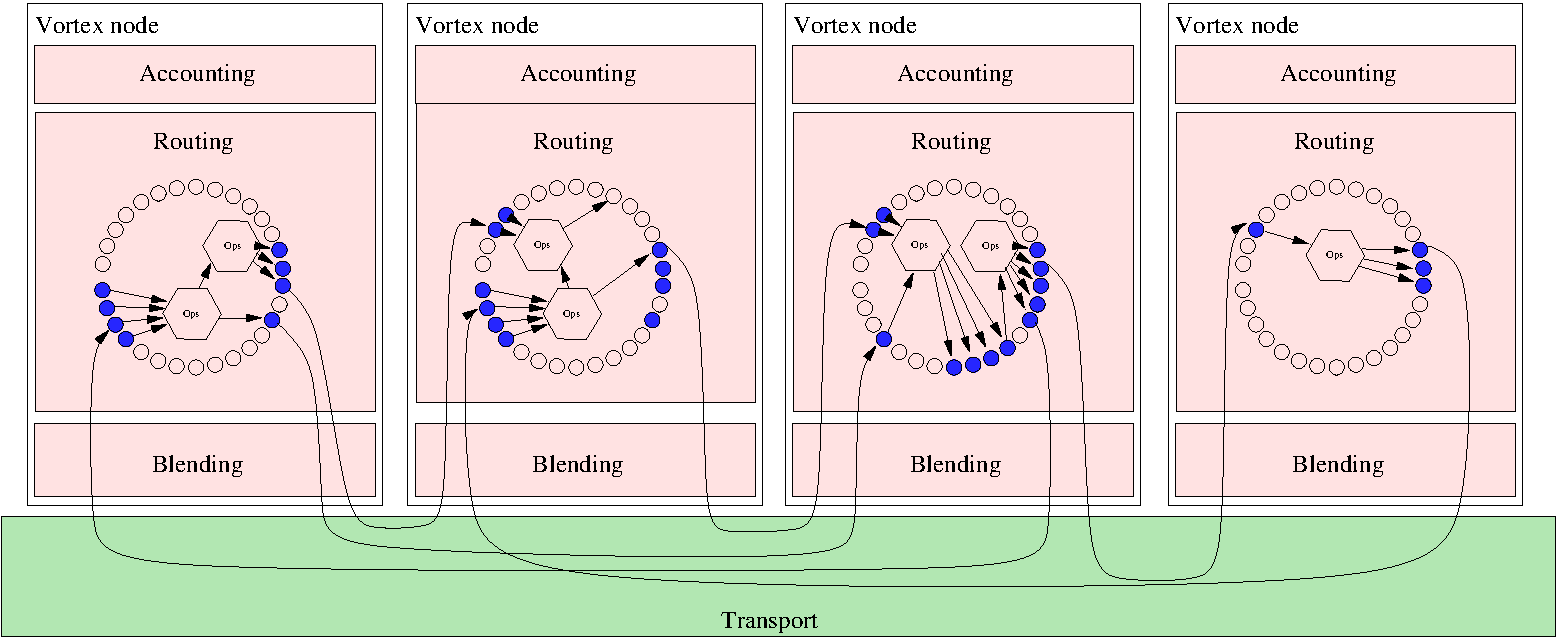
\includegraphics[width=\columnwidth]{inc/roughProtocolDesign.pdf}
	\caption{A generic overview for the protocol showing a circular path of a message}
	\label{fig:roughProtocolDesign}
\end{figure}    

The protocol itself sends messages through a well-known transport protocol (``Transport''). We use this protocol for transporting our messages to the next peer. The messages are hidden within regular messages already using that transport layer. In an ideal implementation, any messages sent by our protocol should be indistinguishable from regular messages (by computers and humans). To achieve this steganographic task, we introduce a ``blending layer''. This layer usually is specific to the underlying transport layer and may vary. We will describe our blending layer implementation in section \ref{sec:blending}.

The ``routing layer'' is the layer that receives and sends messages. It parses only the core protocol, and the data processed here is entirely independent of the underlying transport and blending layer. Our routing layer processes payloads received from VortexMessages with a limited set of predefined operations. The sending node chooses the operations applied to the message.

The ``accounting layer'' disassembles the received messages into its parts. It then recomposes and stores the messages for further routing. We introduce accounting to avoid that unsolicited bulk messages (\defref{UBM}) may be transmitted over our media. This accounting additionally prevents a sender from using up too many resources of any intermediate node. It enables any node to keep control of its resource usage and keeps other nodes from eating up more resources than planned.

The messages passed through such a protocol stack are onionised to offer anonymity from evil nodes. Furthermore, any node or external observer is unable to tell whether a message was intended for a specific other node or not. In consequence, we have to guarantee that all nodes, including sender and recipient, offer the same functions and are indistinguishable.

Operations applied always result in a valid message. As an onionised packet typically loses data on its way, the operations must increase and decrease the message in size to mitigate size tracking attacks. The operations must not leak, which part is a decoy or real parts of the message. Operations not carried out due to missing data might be either intentionally or a malfunction.

The defined message operations are as follows:
\begin{itemize}
	\item Split a message block into two parts of variable size or join them.\\
	We use this operation to fan out decoy traffic, to cut off decoy data, or to send multiple parts of a message through different routing nodes.
	\item Encrypt or decrypt a block with a given key.      
	\item Add and remove redundancy information to a stream\\
	We use this operation to send a message or decoy through multiple channels or recover a partially received message according to the redundancy operation.
\end{itemize}

To avoid making this system attractive to \defref{UBM} and to protect DoS attacks, we introduce accounting to make a mass transfer of data more expensive than other means of message transport. The system works as follows:
\begin{itemize}
	\item Routing nodes may offer their services at a cost. A participating node may pay a fee or solve a crypto-puzzle to pay for these costs.
	\item The following operations may be cost-effective:
	\begin{itemize}
		\item Getting an ephemeral identity (\defref{eID}) on a node (prerequisite for accounting; See section \ref{sec:ephemeralIdentity}).
		\item Assign a maximum number of messages and bytes in a specified interval to an eID on a node.
		\item Offer information about the known routing network by the node.
		\item Offer information about the current quota of an eID.
	\end{itemize}
\end{itemize}
As we want to keep resource consumption for accounting as low as possible, all quotas are limited to a time interval. Such time-bound quotas guarantee that quota data of an accounting layer does not grow indefinitely. It is up to the node to decide what time duration is still acceptable.

We minimize the possibility of an overload attack against a node. We achieve this with the following precautions:
\begin{itemize}
	\item The message build process is far more complex than the routing carried out by the nodes.
	\item Messages may be processed in parts to minimize the amount of work. After processing the start of a message, a node may already decide whether it will route the message or not.
	\item The protocol minimizes the use of inefficient operations (e.g., asymmetric encryption).
	\item The server may limit specific operations.
\end{itemize}

\subsection{Ephemeral Identity\label{sec:ephemeralIdentity}}
We use accounting on various levels. While we are dealing with anonymity, accounting has still to be linked to some identity allowing us to detect malicious actions and ban misbehaving behavior. For this reason, we are introducing a term called ``ephemeral identity'' (\defref{eID}).

\begin{quote}
	An eID is a temporary identity, which is defined by the following attributes:
	\begin{itemize}
		\item It is an identity represented by a public key.
		\item It is only valid for a short, limited time-span.
		\item It is not linkable to another identity of any kind. It is not linkable, especially to the senders' known identity unless this sender is trustworthy, and the sender trusts the infrastructure. Such a trust would always be an exception and is not a prerequisite for successful message transfer.
	\end{itemize}
\end{quote}
The key to this definition is the last point. It is crucial and, at the same time, hard to achieve. In the protocol, any node may request from another node to accept a new eID with a specified quota and a limited lifespan. The node accepting the identity may link its acceptance to the solving of a proof of work puzzle or paying a micro fee in digital currency.

As the \defref{eID}s are limited in their lifespan, a single user has at least one probably multiple \defref{eID}s on any node used directly or indirectly for routing.

\section{Draft of VortexMessages}
For our protocol, we assume the following outline for a message:
\begin{itemize}
	\item Header block\\ 
	This block contains an eID of the sender on the message processing host. It allows the host to decide whether he is willing to process the rest of the message or not. It is essential to know that the identity block contains a symmetric key for decryption of the main block and a secret repeated in the main block. This secret, shared among blocks, keeps a malicious node from exchanging any block.
	\item Routing Blocks\\
	This block contains routing information for all blocks. It furthermore may contain instruction for processing the data blocks and routing/reply blocks for subsequent processing. Routing blocks are not necessarily related to the payload in the same message. They may pick up payloads from other blocks.
	\item payload Block\\
	These Blocks form the payload data. They might contain a message, parts of a message, or decoy material in an unreadable and unidentifiable form.
\end{itemize}

The message is picked up from the transport layer by the blending layer. This layer extracts the contained data with the help of a host key and passes it to the routing layer. The routing layer extracts the message by decrypting the header block. The accounting layer is called to authorize further processing for the identity. If approved, the routing layer adds the routing blocks to the identity-specific workspace. As soon as the time specified in the routing block arrises, the routing block is processed by following the operations specified within. New messages are assembled and sent. The accounting layer keeps track of the \defref{eID}s quota concerning the newly created messages. 

\chapter{Transport Layer Protocol analysis\label{sec:existingTPP}}
In this chapter, we look at the various transport layer protocols. The primary goal is to identify strong candidates as a transport layer. For a full analysis see \ref{app:transportProtocols}.

\section{Crtieria}
When evaluating the transport protocols, we first compiled a list of common messaging protocols. We then analyze these protocols for the following criteria:
\begin{itemize}
	\item Widely adopted (Ct1)\\
	The more widely adopted and used a protocol is, the harder it is for an adversary to monitor (due to the sheer mass), filter, or block the protocol (censorship resistance).
	\item Reliable (Ct2)\\
	Message transport between peers should be reliable. As messages may arrive anytime from everywhere, we do not have means to synchronize the peer partners on a higher level without investing a considerable effort. To avoid this effort, we do look for inherently reliable protocols.
	\item Symmetrical built (Ct3)\\
	The transport layer should rely on a peer to peer base. All servers implement a generic routing that requires no prior knowledge of all possible targets. This criterion neglects centralized infrastructures. This criterion may be dropped, assuming that the blending layer or a specialized transport overlay is responsible for routing.
\end{itemize}

\section{Evaluation Result for Transport Protocols}
\begin{table}[h]
	\centering\tiny
	\begin{tabular}{|l|l|l|l|}\hline
		\diaghead{\theadfont protocol Criteria}{Protocol}{Criteria} & \thead{Ct1: Widely adopted}     & \thead{Ct2: Reliable} & \thead{Ct3: Symmetrically built}\\\hline
		HTTP     & $\checkmark$            & $\checkmark$        & $\times$\\              
		FTP         & $\checkmark$            & $\checkmark$        & $\times$\\
		TFTP     & $\times$                & $\times$            & $\times$\\
		MQTT     & \textasciitilde        & $\checkmark$        & $\times$\\              
		AMQP     & \textasciitilde        & $\checkmark$        & $\times$\\
		CoAP     & \textasciitilde        & \textasciitilde     & $\times$\\
		WAMP     & $\times$                & $\checkmark$        & \textasciitilde\\
		XMPP     & $\checkmark$            & $\checkmark$        & $\checkmark$\\
		SMTP     & $\checkmark$            & $\checkmark$        & $\checkmark$\\\hline
	\end{tabular}    
	\caption{comparison of protocols in terms of the suitability as transport layer}
	\label{tab:protoSuitCrit}
\end{table}

Table \ref{tab:protoSuitCrit} sums up all previously analyzed protocols in section \ref{app:transportProtocols}. We use ``$\checkmark$'' for a fulfilled criterion, ``\textasciitilde'' for a partially fulfilled criterion, and ``$\times$'' for a not fulfilled criterion. This overview shows in compact form protocols identified as strong candidates for use as a transport layer in terms of an anonymizing protocol. 

This table shows that strong identified candidates are \defref{SMTP} (being already a message sending protocol on asynchronous base) and \defref{XMPP} (a real-time chat protocol able to attach files). Both have the advantages that they are widely adopted on the Internet and do additional support content (such as alternatives or attachments).

If assuming an implemented transport layer overlay on the MessageVortex protocol side, HTTP and FTP are suitable candidates as well.

\chapter{Existing Research and Implementations on the Topic \label{sec:existingRD}}
\section{Anonymity Research}
In this section, we collect protocols research related to anonymity. We did not stick to anonymous message transfer. Instead, we took a broad focus in terms of technology and outlined in each protocol strengths and weaknesses identified, which may be relevant to this research.

\subsection{Definition of Anonymity}
As the definition for Anonymity we take the definition as specified in \cite{anonTerminology}.\DeclareFixedFootnote{\omitted}{footnotes omitted in quote}
\begin{quote}
	Anonymity of a subject means that the subject is not identifiable within a set of subjects, the anonymity set.\omitted
\end{quote}
and
\begin{quote}
	Anonymity of a subject from an attacker's perspective means that the attacker cannot sufficiently identify the subject within a set of subjects, the anonymity set.\omitted
\end{quote}

We define the anonymity set as the set of all possible subjects within a supposed message. The anonymity of a subject towards an observing third party is a crucial factor as it relates directly to our adversary model.

\subsection{\texorpdfstring{$k$}{k}-Anonymity}
$k$-anonymity is a term introduced in \cite{k-anonymous:ccs2003}. This work claims that entities are not responsible for an action if an observer is unable to match a specific action to less than $k$ entities.

The Document distinguishes between \textit{Sender $k$-anonymity}, where the sending entity can only be narrowed down to a set of $k$ entities and \textit{Receiver $k$-anonymity}. 

The size of $k$ is a crucial factor. One of the criteria is the legal requirements of the jurisdiction. Depending on the jurisdiction, it usually is not possible to prosecute someone if an action is not directly coupled to one person. Another criterion might be the decreasing of $k$ over time. If a Vortex account is used, we have to assume that some vortex identities go out of commission over time. If $k$ is chosen according to a legal requirement, it should be taken into account that $k$ might be decreasing over time.

\subsection{\texorpdfstring{$\ell$}{l}-Diversity}
In \cite{machanavajjhala2007diversity} an extended model of $k$-anonymity is introduced. In this paper, the authors emphasize that it is possible to break a $k$-anonymity set if there is additional information available which may be merged into a data set so that a distinct entity can be filtered from the $k$-anonymity set. In other words, if an anonymity set is to tightly specified, additional background information might be sufficient to identify a specific entity in an anonymity set.

It might be arguable that a $k$-anonymity in which a member is not implicitly $k$-anonymous still is sufficient for $k$-anonymity in its sense. However, the point made in this work is right and is taken into account. Their approach is to introduce an amount of invisible diversity into $k$-anonymous sets, so that common background knowledge is no longer sufficient to isolate a single member.

\subsection{\texorpdfstring{$t$}{t}-Closeness}
While $\ell$-diversity protects the identity of an entity, it does not prevent information gain. A subject which is in a class has the same attributes. This is where $t$-closeness\cite{li2007t} comes into play. $t$-closeness is defined as follows:

\begin{quote}
	An equivalence class is said to have $t$-closeness if the distance between the distribution of a sensitive attribute in this class and the distribution of the attribute in the whole table is no more than a threshold. A table is said to have $t$-closeness if all equivalence classes have $t$-closeness.
\end{quote}

\section{Single Use Reply Blocks and Multi-Use Reply Blocks}
Chaum first introduced the use of reply blocks in \cite{CHAUM1}. A routing block, in general, is a structure allowing to send a message to someone without knowing the targets' real address. Reply blocks may be differentiated into two classes ``Single Use Reply Blocks'' (SURBs)  and ``Multi-Use Reply Blocks'' (MURBs). SURBs may be used once while MURBs may be used a limited number of times. 

Within our research, we discovered that if a routing protocol is reproducible, the traffic of a MURB may be used to identify some of the properties of the message. Depending on the type of attack, the block has to be repeated very often. For this reason, we limited the number of replays to a low number. The concept is that we have, in our case a routing block, which might be used up to $n$ times ($0<n<127$). It is easily representable in a byte integer (signed or unsigned) on any system. It is big enough to support human communication sensibly and is big enough to add not too much overhead when rerequesting more MURBs. The number should not be too big because if a MURB is reused, the same pattern of traffic is generated, thus making the system susceptible to statistical attacks.

\section{Censorship}
As a definition for censorship we take
\begin{quote}
	Censorship: the cyclical suppression, banning, expurgation, or editing by an individual, institution, group or government that enforce or influence its decision against members of the public -- of any written or pictorial materials which that individual, institution, group or government deems obscene and ``utterly without redeeming social value,'' as determined by ``contemporary community standards.''
\end{quote}

The definition is attributed to Chuck Stone Professor at the School of Journalism and Mass Communication, University of North Carolina. Please note that ``Self Censorship'' (not expressing something in fear of consequences) is a form of censorship too.

In our more technical we reduce the definition to
\begin{quote}
	Censorship: A systematic suppression, modification, or banning of data in a network by either removal, or modification of the data, or systematic influencing of entities involved in the processing (e.g., by creating, routing, storing, or reading) of this data.
\end{quote}
This simplified definition narrows down the location to the Internet as it is the only relevant location for us.  Furthermore, it limits the definition to the maximum reach within that system.

\subsection{Censorship Resistant}
A censorship-resistant system is a system that allows the entities of the system and the data itself to be unaffected from censorship. Please note that this does not deny the presence of censorship per se. It still exists outside the system. However, it has some consequences for the system itself.

\begin{itemize}
	\item The system must be either undetectable or out of reach for an entity censoring.\\
	The possibility of identifying a protocol or data allows a censoring entity to suppress the use of the protocol itself. 
	\item The entities involved in a system must be untraceable.\\
	Traceable entities would result in a mean of suppressing real-world entities participating in the system.
\end{itemize}

\subsection{Parrot Circumvention}
In \cite{oakland2013-parrot} \citeauthor{oakland2013-parrot} express that it is easy for a human to determine decoy traffic as the content is easily identifiable as generated content. While this is true, there is a possibility here to generate ``human-like'' data traffic to a certain extent. As an adversary may not assume that his messages are replied to, the problem does not boil down to a true Turing test. It remains on a ``passive observer Turing test'', enabling the potential nodes to choose their messages. 

In our design, this is the job covered by the blending layer. The blending layer generates these messages. These messages are context-less or remain in the context of previous conversations.

\subsection{Censorship Circumvention}
Several technical ways have been explored to circumvent censorship. All seem to boil down to the following main ideas:
\begin{itemize}
	\item Hide data
	\item Copy or distribute data to a vast amount of places to improve the lifespan of data
	\item Outcurve censorship measurements
\end{itemize}

In the following section, we look at technologies and ideas dealing with these circumvention technologies.

\subsubsection{Covert Channel and Channel Exploitations}
The original term of covert channels was defined by \citeauthor{Lampson73anote}\cite{Lampson73anote} as 

\begin{quote}
	not intended for information transfer at all, such as the service program's effect on system load.
\end{quote}

This was defined  in such a way to distinguish the message flow from 

\begin{quote}
	legitimate channels used by the confined service, such as the bill.
\end{quote}

The use of a legitimate channel such as \defref{SMTP} and hide information within this specific channel is not a usage of a covert channel. We refer to this as channel exploitation.

\subsubsection{Steganography}

Steganography is an important part when it comes to unlinking information. In \cite{6828087} and \cite{subhedar2014current} we get a very rough overview. As some of the types and algorithms address specific topics of steganography (e.g., some hide from automatic detection and others address a human message stream auditor), we need to choose carefully. In our specific case, the main idea is to hide within the sheer mass of Internet traffic. As a human auditor screening all the messages is a minor thread, we focus on machine-based censorship. Most of the images sent in \defref{SMTP} are jpg images (see table \ref{tab:emailAttachments} on page \pageref{tab:emailAttachments}). We limited our search to algorithms capable of hiding binary data within these files. The number of academically researched options was surprisingly low.

After reviewing the options, we decided to go for F5\cite{f5}. It is a reasonably well-researched algorithm which attracted many researchers. The original F5 implementation had a detectable issue with artifacts\cite{F5broken} caused by the recompression of the image. This issue was caused only due to a problem in the reference implementation, and the researchers have provided a corrected reference implementation without the weakness.

% We use https://github.com/matthewgao/F5-steganography

YASS, as described in \cite{solanki2007yass}, was not considered a candidate. Although less researched, researchers found multiple weakness\-es\cite{kodovsky2010modern,li2009steganalysis}.

\subsubsection{Timing Channels}

Timing channels are a specialized form of covert channels. In timing channels, the information itself hides not within the data of the channel, but the usage of the channel is in such a way that it is capable of reflecting the data. As we do not have control over the timing of the transport channel, this is not an option for us.

\section{Cryptography}

Whenever dealing with obfuscating data and maintaining the integrity of data, cryptography is the first tool in the hand of an implementer. A vast amount of research in this area does already exist. For this work, we focussed on algorithms either very well researched and implemented or research, which seem very valuable when putting this work into place. 

In symmetric encryption in this paper always assumes that
\begin{eqnarray}
D^{K_a}\left(E^{K_a}\left(\mathbf{M}\right)\right) & = & \mathbf{M}
\end{eqnarray} 

For a key $K_b\neq K_a$ this means

\begin{eqnarray}
D^{K_a}\left(E^{K_b}\left(\mathbf{M}\right)\right) & \neq & \mathbf{M}\\
D^{K_b}\left(E^{K_a}\left(\mathbf{M}\right)\right) & \neq & \mathbf{M}
\end{eqnarray} 

The following candidates have been analyzed:
\begin{itemize}
	\item AES\\
	NIST announced AES in \citeyear{standard2001announcing} as a result of a contest. The algorithm works with four operations (subBytes, ShiftRows, mixColumns, and addRoundKey). These operations are repeated depending on the key length 10 to 14 times. 
	
	AES is up until now (2018) unbroken. It has been weakened in the analysis described in \cite{tao2015improving}, which reduces the complexity by roughly one to two bits. 
	
	\item Camellia\\
	The camellia algorithm is described in \cite{RFC3713}. The key sizes are 128, 192, and 256. Camellia is a Feinstel cipher with 18 to 24 rounds depending on the key size. Up until today, no publication claims break this cipher. 
\end{itemize}

For all asymmetric encryption algorithm in this paper, we may assume that\ldots

\begin{eqnarray}
D^{K^{-1}_a}\left(E^{K^{1}_a}\left(\mathbf{M}\right)\right) & = & \mathbf{M}\\
D^{K^{1}_a}\left(E^{K^{-1}_a}\left(\mathbf{M}\right)\right) & = & \mathbf{M}
\end{eqnarray} 

It is important that 
\begin{eqnarray}
D^{K^{-1}_a}\left(E^{K^{-1}_a}\left(\mathbf{M}\right)\right) & \neq & \mathbf{M}\\
D^{K^{1}_a}\left(E^{K^{1}_a}\left(\mathbf{M}\right)\right)   & \neq & \mathbf{M}
\end{eqnarray} 

And for any other Keypair $K^{p}_a \neq K^{p}_b$
\begin{eqnarray}
D^{K^{-1}_b}\left(E^{K^{1}_a}\left(\mathbf{M}\right)\right)  & \neq & \mathbf{M}\\
D^{K^{1}_b}\left(E^{K^{1}_a}\left(\mathbf{M}\right)\right)   & \neq & \mathbf{M}\\
D^{K^{-1}_b}\left(E^{K^{-1}_a}\left(\mathbf{M}\right)\right) & \neq & \mathbf{M}\\
D^{K^{1}_b}\left(E^{K^{-1}_a}\left(\mathbf{M}\right)\right)  & \neq & \mathbf{M}
\end{eqnarray} 

The number of crypto algorithms was higher than the steganography options. When looking for well-researched algorithms basing on different mathematical problems and having well-defined outlines, numbers dropped dramatically again.

\begin{itemize}
	\item RSA\\
	In \citeyear{Rivest:1978:MOD:359340.359342} the authors \citeauthor{Rivest:1978:MOD:359340.359342} published with \cite{Rivest:1978:MOD:359340.359342} a paper which did revolutionize cryptography for years. In their paper, the authors described an encryption method later to be called RSA, which required a key pair ($K_a$) referenced as public ($K^{1}_a$) and private keys ($K^{-1}_a$). The novelty of this system was that anything encrypted with the public key was only decryptable with the private key and vice versa.
	
	RSA is up until the day of writing this paper not publicly know to be broken (unless a too small key size is used). However -- \citeauthor{Shor97polynomial-timealgorithms} described in \citeyear{Shor97polynomial-timealgorithms} an algorithm which should enable quantum computers to break RSA far faster than done with traditional computers. In the section \ref{sec:keySize} we do elaborate these effects further.
	\item ECC\\
	The elliptic curves were independently suggested by \cite{Miller1986} and \cite{Koblitz04guideto} in 1986. Elliptic curve Cryptography started to be widely deployed in the public space in 2006. Since then, it seems to compete very well with the well established RSA algorithm. While being similarly well researched ECC, has the advantage of far shorter key sizes for the same grade of security.
	\item McElliece\\
	McEliece was first implemented and then removed again. The key size to gain equivalent security to RSA1024 was $\approx 1MB$. This was impractical and thus discarded again. This was done, although there is up until now no known quantum capable algorithm reducing the key size of McEliece.
	\item NTRU\\
	In \cite{Hoffstein1998} \citeauthor{Hoffstein1998} described the NTRU algorithm. The inclusion of this algorithm was disputed as it is patented in the united states as US7031468. It was included because the company Security Innovation holding the patent, released the NTRU algorithm on March \thanks{28} 2018 into the public domain according to a blog entry on the company website. While NTRU is not as well researched as RSA, it has been around for more than 20 years without being significantly affected by known attacks.
	\item ElGammal\\
	We rejected ElGamal as a cryptosystem to include. It bases on the same mathematical problems for cryptoanalysis as RSA (discreet logarithms) but is not as common as RSA.
\end{itemize}


\subsection{Homomorphic encryption}
Homomorphic encryption, as introduced in \cite{feldman1987practical}, was from the beginning a strong candidate to be used within our work. Unfortunately, we did not find a way to apply the core addRedundancy operation in homomorphic encryption. Transforming the original data to the GF space in an efficient way to apply matrices was not doable and thus rejected.

%\cite{Gentry:2009:FHE:1536414.1536440} %FIXME dangling reference

\subsection{Deniable Encryption and Deniable Steganography}

Deniable encryption and deniable steganography have been considered out-of-bounds for this work. The main reason is that the presence of encryption (which is not deniable in both cases) may be sufficient for a censor to block a message. Adding a layer to make sure that encryption or steganography is deniable, does not add valuable properties to our system as the sheer presence of encryption might be sufficient for censorship. 

\subsection{Key Sizes\label{sec:keySize}}

The question of key sizes is hard to answer as it depends on the current and future possibilities of an adversary, which is again depending on not foreseeable research. We tried to collect a couple of recommendations.

\href{http://www.ecrypt.eu.org/}{Encrypt II (http://www.ecrypt.eu.org/)} recommends currently for a ``foreseeable future'' 256 Bits for symmetric encryption and for asymmetric encryption based on factoring modulus 15424 Bits. Elliptic Curve Cryptography and Hashing should be sufficient if used with at least 512 Bits. If the focus is reduced to the next $\approx$ 20 years, then the key size recommendations are reduced to 128 Bit for symmetric encryption, 3248 Bits for factoring modulus operations, and 256 Bits for elliptic curves and hashing.

According to the equations proposed by \citeauthor{Lenstra04keylength.} in \cite{Lenstra04keylength.} an asymmetric key size of 2644 Bits respectively symmetric key length of 95 Bits, or 190 Bits for elliptic curves and hashing should be sufficient for security up to the year 2048. 

According to \cite{CNSASuite} (superseding well known and often used \cite{nsa-fact-sheet-B}) data classified up to ``top secret'' should be signed with RSA 3072+ or ECDSA P-384.  For symmetric encryption, they recommend AES 256 Bits, for Hashing at least SHA-384 and for Elliptic curves a 384 Bit sized key.

As it might seem not a wise idea to consider the recommendation of a potential state-sponsored adversary and the Formulas proposed by \citeauthor{Lenstra04keylength.} do not explicitly take quantum computers into account, we follow the advice of ENCRYPT II.

Furthermore, taking all recommendations together, it seems that all involved parties assume the most trust in elliptic curves rather than asymmetric encryption based on factoring modulus.

\subsection{Cipher Mode}
The cipher mode defines how multiple blocks encrypted with the same key are handled. Main characteristics of cipher modes to us are:
\begin{itemize}
	\item Parallelisable\\ 
	Can multiple parts of a plaintext be encrypted simultaneously? This feature is important for multi CPU and multi-core systems as they can handle parallelizable more efficiently by distributing them on multiple CPUs.
	\item Random access in decryption\\
	Random access on decryption allows efficient partial encryption of a ciphertext.
	\item Initialisation vector\\
	An initialization vector has downsides and advantages. On the downsides is the fact that an initialization vector must be shared with the message or before distributing it. It is essential to understand that the initialization vector itself usually is not treated as a secret. It is not part of the key.
	\item Authentication\\
	Authentication guarantees that the deciphered plaintext has been unmodified since encryption. It does not make a statement over the identity of the party encrypting the text. Such an identifying authentication is referred to as signcryption.
\end{itemize}

We evaluated the most common cipher modes for suitability. For MessageVortex, we focussed on modes that have the properties parallelizable, random access, and do not do authentication. The main focus, besides the characteristics mentioned above, was on the question of whether there is an open implementation available in java, which is reasonably tested.

\begin{itemize}
	\item ECB (Electronic Code Book)\\
	ECB is the most basic mode. Each block of the cleartext is encrypted on its own. This results in a big flaw: blocks containing the same data will always transform to the same ciphertext. This property makes it possible to see some structures of the plain text when looking at the ciphertext. This solution allows the parallelization of encryption, decryption, and random access while decrypting. Due to these flaws, we rejected this mode.
	\item CBC (Cypher Block Chaining)\\  
	CBC extends the encryption by xor'ing an initialization vector into the first block before encrypting. For all subsequent blocks, the ciphertext result of the preceding block is taken as xor input. This solution does not allow parallelization of encryption, but decryption may be paralleled, and random access is possible. As another downside, CBC requires a shared initialization vector. As with most IV bound modes, an IV/key pair should not be used twice, which has implications for our protocol.
	\item PCBC (Propagation Cypher Block Chaining)\\
	CBC extends the encryption by xor'ing, not the ciphertext but a xor result of ciphertext and plaintext. This modification denies parallel decryption and random access compared to CBC.
	\item EAX\\      
	EAX has been broken in 2012\cite{minematsu2013attacks} and is therefore rejected for our use.
	\item CFB (Cypher Feedback)
	CFB is specified in \cite{dworkin2001recommendation} and works precisely as CBC with the difference that the plain text is xor'ed and the initialization vector, or the preceding cipher result is encrypted. CFB does not support parallel encryption as the ciphertext input from the preceding operation is required for an encryption round. CFB does, however, allow parallel decryption and random access.
	\item OFB\\
	\cite{dworkin2001recommendation} specifies OFB and works exactly as CFB except for the fact that not the ciphertext result is taken as feedback but the result of the encryption before xor'ing the plain text. This denies parallel encryption and decryption, as well as random access.
	\item OCB (Offset Codebook Mode)\\
	This mode was first proposed in \cite{rogaway2003ocb} and later specified in \cite{krovetz-ocb-04}. OCB is specifically designed for AES128, AES192, and AES256. It supports authentication tag lengths of 128, 96, or 64 bits for each specified encryption algorithm. OCB hashes the plaintext of a message with a specialized function $H_{OCB}(\mathbf{M})$. OCB is fully parallelizable due to its internal structure. All blocks except the first and the last can be encrypted or decrypted in parallel.
	\item CTR\\
	CTR is specified in \cite{lipmaa2000ctr} and is a mixture between OFB and CBC. A nonce concatenated with a counter incrementing on every block is encrypted and then xor'ed with the plain text. This mode allows parallel decryption and encryption, as well as random access. Reusing IV/Key-pairs using CTR is a problem as we might derive the xor'ed product of two messages. This problem only applies where messages are not uniformly random such as in an already encrypted block.
	\item CCM\\
	Counter with CBC-MAC (CCM) is specified in \cite{RFC3610}. It allows to pad and authenticate encrypted and unencrypted data. It furthermore requires a nonce for its operation. The size of the nonce is dependent on the number of octets in the length field. In the first 16 bytes of the message, the nonce and the message size is stored. For the encryption itself, CTR is used. It shares the same properties as CTR. 
	
	It allows parallel decryption and encryption as well as random access.
	\item GCM (Galois Counter Mode)\\
	GCM has been defined in \cite{mcgrew2004galois}, and is related to CTR but has some major differences. The nonce is not used (just the counter starting with value 1). To authenticate the encryption, an authentication token $auth$ is hashed with $H_{GFmult}$ and then xor'ed with the first cipher block. All subsequent cipher blocks are xor'ed with the previous result and then hashed again with $H_{GFmult}$. After the last block the output $o$ is processed  as follows: $H_{GFmult}(o\bigoplus (len(A)||len(B))) \bigoplus E^{K^0}(counter_0)$. As a result, GCM is not parallelizable and does not support random access.
	
	The mode has been analyzed security-wise in \citeyear{mcgrew2004security} and showed no weaknesses in the analyzed fields \cite{mcgrew2004security}. 
	
	GCM supports parallel Encryption and decryption. Random access is possible. However, authentication of encryption is not parallelizable. The authentication makes it unsuitable for our purposes. Alternatively, we could use a fixed authentication string.
	\item XTS (XEX-based tweaked-codebook mode with ciphertext stealing)\\
	This mode is standardized in IEEE 1619-2007 (soon to be superseded). A rough overview of XTS may be found at \cite{Martin2010}. It was developed initially for Disks offering random access and authentication at the same time. 
	\item CMC (CBC-mask-CBC) and EME (ECB-mask-ECB)\\ 
	In \cite{Halevi:2003} \citeauthor{Halevi:2003} introduces a cipher mode which is extremely costly as it requires two encryptions. CMC is not parallelizable due to the underlying CBC mode, but EME is. 
	\item LRW\\
	LRW is a tweakable narrow-block cipher mode described in \cite{tschorsch:translayeranon}. This mode shares the same properties as EBC but without the weakness of the same clear text block resulting in the same ciphertext. Similarly to XEX, it requires a tweak instead of an IV.
\end{itemize}

\subsubsection{Summary of Cipher Modes}

\begin{table}[ht]
	\centering\tiny
	\begin{tabular}{|l|l|l|l|l|}\hline
		\diaghead{\theadfont Mode Criteria}{Mode}{Criteria}         & \thead{auth}  &\thead{Requires IV}               & \thead{parallelisable}     & \thead{random access}\\
		\hline
		CBC                                                            & $\times$        & $\checkmark$                      & $\times$                & $\times$\\                      
		CCM                                                            & $\times$        & $\checkmark$                      & $\times$                   & $\times$\\
		CFB                                                            & $\times$        & $\checkmark$                      & $\checkmark$            & $\checkmark$\\              
		CTR                                                            & $\times$        & $\checkmark$                      & $\checkmark$               & $\checkmark$\\              
		ECB                                                            & $\times$        & $\times$                          & $\checkmark$            & $\checkmark$\\   
		GCM                                                            & $\checkmark$    & $\checkmark$                      & $\times$                   & $\times$\\              
		OCB          & $\checkmark$& $\times$\footnotemark[1]    &$\times$                    &$\times$\\
		OFB          & $\times$    & $\checkmark$                &$\times$                    &$\times$\\
		PCBC         & $\times$    & $\checkmark$                &$\times$                    &$\times$\\
		XTS          & $\times$    & $\checkmark$\footnotemark[2]&$\checkmark$                &$\times$\\
		LRW          & $\times$    & $\checkmark$\footnotemark[2]&$\checkmark$                & $\checkmark$\\
		CMC          & $\times$    & $\checkmark$\footnotemark[2]& $\times$                   & $\times$\\
		EME          & $\times$    & $\checkmark$\footnotemark[2]& $\checkmark$                    & $\checkmark$\\              
		\hline          
	\end{tabular}    
	\caption{comparison of encryption modes in terms of the suitability}
	\label{tab:ModeSuitCrit}
\end{table}
\footnotetext[1]{included in auth}
\footnotetext[2]{Requires tweak instead of IV}

\subsection{Padding}
A plain text stream may have any length. Since we always encrypt in blocks of a fixed size, we need a mechanism to indicate how many bytes of the last encrypted block may be safely discarded. 

Different paddings are used at the end of a cipher stream to indicate how many bytes belong to the decrypted stream.

\subsubsection{RSAES-PKCS1-v1\_5 and RSAES-OAEP}
This padding is the older of the paddings standardized for PKCS1. It is basically a prefix of two bytes followed by a padding set of non zero bytes and then terminated by a zero byte and then followed by the message. This patting may give a clue if decryption was successful or not. RSAES-OAEP ist the newer of the two padding standards 

\subsubsection{PKCS7} 
This padding is the standard used in many places when applying symmetric encryption up to 256 bits key length. The free bytes in the last cipher block indicate the number of bytes being used. This makes this padding very compact. It requires only 1 Byte of functional data at the end of the block. All other bytes are defined but not needed.

\subsubsection{OAEP with SHA and MGF1 padding} 
This padding is closely related to RSAES-OAEP padding. The hash size is, however, bigger, and thus, the required space for padding is much higher. OAEP with SHA and MGF1 Padding is used in asymmetric encryption only. Due to its size, it is important to note that the payload in the last block shrinks to $keySizeInBits/8-2-MacSize/4$.

In our approach, we have chosen to allow these four paddings. The allowed sha sizes match the allowed mac sizes chosen above. It is important to note that padding costs space at the end of a stream. Since we are always using one block for signing, we have to take care that the chosen signing mac plus the bytes required for padding do not exceed the key size of the asymmetric encryption. While this usually is not a problem for RSA as there are keys 1024+ Bits required, it is an essential problem for ECC algorithms as there are much shorter keys needed to achieve an equivalent strength compared to RSA. 

We have introduced an additional type of padding not related to these paddings. We required for the addRedundancy the following unique properties. Unfortunately, we were unable to find any padding which matched the following properties simultaneously:

\begin{itemize}
	\item Padding must not leak successful decryption\\
	For our addRedundancy operation, we required padding that had no detectable structure as a node should not be able to tell whether a removeRedundancy operation did generate content or decoy. 
	\item Padding of more than one block\\
	Due to the nature of the operation, it is required to be able to pad more than just one block.
\end{itemize}

Details of this padding are described in the section "Add and Remove Redundancy Operations'' in \ref{app:rfcMessageVortexMain}. 

\section{Routing}

If we can follow data from a source to a destination, we may safely assume that the participants of this data exchange are no longer anonymous. So special care should be taken to this aspect. In the past, several approaches have been made to avoid the detection of data while routing. In the following sections, we will look at some basic concepts which have been proposed up until today. We describe their idea and have a look at their weaknesses discovered so far.

In \nameref{sec:sysImpl}, we analyze some related real-world systems regarding how they work and how they have been attacked in the past.

\subsection{Mixing\label{sec:mixnets}}
Mixes have been first introduced by \citetitle{CHAUM1}\cite{CHAUM1} in \citeyear{CHAUM1}. The basic concept in a mix goes as follows. We do not send a message directly from the source to the target. Instead, we use a kind of proxy server or router in between which picks up the packet, anonymizes it, and forwards it either to the recipient or another mix. If we assume that we have at least three mixes cascaded, we then can conclude that:
\begin{itemize}
	\item Only the first mix knows the true sender
	\item All intermediate mixes know neither the true sender nor the true recipient (as the data comes from mixes and is forwarded to other mixes) 
	\item Only the last mix knows the final recipient.
\end{itemize}

This approach (in this simple form) has several downsides and weaknesses.

\begin{itemize}
	\item In a low latency network, the message may be traced by analyzing the timing of a message.
	\item We can emphasize a path by replaying the same message multiple times (assuming we control an evil node), thus discovering at least the final recipient.
	\item If we can ``tag'' a message (with content or attribute), we then may be able to follow the message.
\end{itemize}

In \citeyear{RP03-1} \citeauthor{RP03-1} analyzed the suitability for mixes as an anonymizing network for masses. They concluded that there are three possibilities to run mixes.
\begin{itemize}
	\item Commercial, static MixNetworks
	\item Static MixNetworks operated by volunteers
	\item Dynamic MixNetworks
\end{itemize}
They concluded that in an ideal implementation, a dynamic mix network where every user is operating a mix is the most promising solution as static mixes always might be hunted by an adversary.

\subsection{Onion Routing}
Onion routing is a further development of the concept of mixes. In onion routers, every mix gets a message which is asymmetrically encrypted. By decrypting the message, he gets the name of the next-hop and the content which he has to forward. The main difference in this approach is that in traditional mix cascades, the mix decides about the next hop. In an onionised routing system, the message decides about the route it is taking. 

While tagging attacks are far harder (if we exclude side-channel attacks to break sender anonymity), the traditional attacks on mixes are still possible. So when an adversary is operating entry and exit nodes, it is straightforward for them to match the respective traffic.

One very well known onion routing network is Tor (\href{https://www.torproject.org}{https://www.torproject.org}). For more information about tor see section \ref{sec:tor}.

\subsection{Crowds}

Crowds is a network that offers anonymity within a local group. It works as follows:

\begin{itemize}
	\item All users add themselves to a group by registering on a so-called ``blender''.
	\item All users start a service (called JonDo).
	\item Every JonDo takes any received message (might be from him as well) and sends it with a 50\% chance either to the correct recipient or to a randomly chosen destination
\end{itemize}

While crowds as specified in \cite{crowds:tissec} does anonymize the sender from the recipient rather well, the system offers no protection from someone capable of monitoring crowds traffic. The system may, however, be easily attacked from within by introducing collaborating johndos. It has been further developed to D-Crowds \cite{DBLP:conf/esorics/DanezisDKT09}, ADU/RADU \cite{Munoz-Gea2008}, Freenet\cite{freenet} and others. 

Furthermore, the blender is aware of all JonDos and thus of particular interest for any observing or censoring adversary. Control of the blender enables an adversary to split the network into controllable parts, adding a high likelihood of discovering an original sender.

\subsection{Mimic routes}
Mimics are a set of statical mixes which maintain a constant message flow between the static routes. If legitimate traffic arrives, the pseudo traffic is replaced by legitimate traffic. An outstanding observer is thus incapable of telling the difference between real traffic and dummy traffic.

If centralized mixes are used, the system lacks the same vulnerabilities of sizing and observing the exit nodes as all previously mentioned systems. If we assume that the sender and receiver operate a mixer by themselves, the system would no longer be susceptible to timing or sizing analyses. The mimic routes put a constant load onto the network. This bandwidth is lost and may not be reclaimed. It does not scale well as every new participant increases the need for mimic routes and creates (in the case of user mixes) a new mimic load. Furthermore, the mixes are easily identifiable as their characteristic data stream contrasts compared to other network service streams.

\subsubsection{DC Networks}
DC networks are based on the work \citetitle{chaum-dc} by \citeauthor{chaum-dc}\cite{chaum-dc}. In this work, \citeauthor{chaum-dc} describes a system allowing a one-bit transfer (The specific paper talks about the payment of a meal). Although all participants of the DC net are known, the system makes it unable to determine who has been sending a message. The message in a DC-Net is readable for anyone. This network has the downside that a cheating player may disrupt communication without being traceable.

Several attempts have been made to strengthen the proposal of Chaum\cite{golle:eurocrypt2004,disco,herbivore:tr,Corrigan-Gibbs:2010:DAA:1866307.1866346}. However, no one succeeded without introducing significant downsides on the privacy side.
\subsubsection{Annonymous Remailer\label{sec:remailer}}
Remailers have been in use for quite some time. There are several classes of remailers, and all of them are somehow related to Mixnets. There are ``types'' of remailers defined. Although these ``types'' offer some hierarchy, none of the more advanced ``types'' seem to have more than one implementation in the wild. 

Pseudonymous Remailers (also called Nym Servers) take a message and replace all information pointing to the original sender with a pseudonym. This pseudonym may be used as an answer address. The most well known pseudonymous remailer possibly was anon.penet.fi run by Johan Helsingius. This service has been forced several times to reveal a pseudonyms true identity before Johan Heösingius decided to shut it down. For a more in-depth discussion of Pseudonymous Remailers see \ref{sec:remPseudo}

Cypherpunk remailers forward messages like pseudonymous remailers. Unlike pseudonymous remailers, Cypherpunk remailers decrypt a received message, and its content is forwarded without adding a pseudonym. A reply to such a message is not possible. They may, therefore, be regarded as an ``decrypting reflector'' or a ``decrypting mix'' and may be used to build an onion routing network for messages. For a more in-depth discussion of type-1-remailers, see section  \ref{sec:remCypherpunk}.

Mixmaster remailers are very similar to Cypherpunk remailers. Unlike them, Mixmaster remailers hide the messages, not in an own protocol, but use \defref{SMTP} instead. While using \defref{SMTP} as a transport layer, Cypherpunk remailers are custom (non-traditional mail) servers listening on port 25. For a more in-depth discussion of type-2-remailers, see section \ref{sec:remMixmaster}.

Mixminion remailers extend the model of Mixmaster remailers. They still use \defref{SMTP} but introduce new concepts. New concepts in Mixminion remailers are:
\begin{itemize}
	\item Single Use Reply Blocks (SURBs)
	\item Replay prevention
	\item Key rotation
	\item Exit poicies
	\item Dummy traffic
\end{itemize}
For a more in depth discussion of Mixminion remailers see section \ref{sec:remMixminion}.

\section{System Implementations\label{sec:sysImpl}}
The following sections emphasize on implementations of anonymizing (and related) protocols regardless of their usage in the domain of messaging and anonymity. It is a list of system classes or their specific implementations together with a short analysis of strengths and weaknesses. 

Wherever possible, we try to refer to sources. If systems are no longer in use or have never been adopted outside the scientific community, we try to refer to publicly available sources. Some of them do not even have a rudimentary implementation. Instead, they are limited to an idea or a simulator.

If a system shows strong similarities in parts, then we emphasize on these parts and analyze the findings and attacks.

All systems have in common that they are easily identifiable on the network layer except for ToR when working with ``pluggable transports'.'

\subsection{Pseudonymous Remailer\label{sec:remPseudo}}
The basic idea of remailers was discussed in \cite{CHAUM1}. The most well-known remailer was probably anon.penet.fi, which operated from 1993 to 1996. This type of remailer is often referred to as type-0-remailer.

In principle, an anonymous remailer works as an ordinary forwarding \defref{SMTP} server. The only difference is that it strips off all header fields except for ``from'', ``to'', and ``subject'' and then replaces the sender and recipient address with pseudonyms respectively with the real address. 

This kind of remailer is easily attackable by an authority. Since the remailer knows tuples of pseudonyms and their respective real identities, it was forced in the past to reveal true identities\cite{penetClosure}. Furthermore, the message may be monitored at the server or on its way, and then due to the unmodified content matching is easy.

This remailer offers, therefore, no protection against an adversary defined in our problem.

\subsection{Babel}
Babel was an academic system defined in a paper by \citeauthor{babel} in \citeyear{babel}\cite{babel}. It has been developed at IBM Zurich Research Laboratory. It was a mixing system using onionized addresses. The sender remains anonymous while he may provide a reply routing block called RPI. If both parties would like to remain anonymous, the RPI of the initiator is deployed in a forum thread. Anyone using this block adds an RPI for its address to the message.

This system has all the disadvantages of a system using MURBs. Traffic highlighting and similar attacks are possible.

\subsection{Cypherpunk-Remailer\label{sec:remCypherpunk}}
With the failing of anon.penet.fi, it became clear that the weakest spot of a single server infrastructure the information stored on the server and the vulnerability of their owner. The new type-1-remailers score over the existing type-1-remailers by using encryption for the message. By combining multiple type-1-remailers, an onion-like structure of the message was achievable. 

This approach was promising, but it was still observable. An observation was possible in the example of correlating the message sizes and timing information.

\subsection{Mixmaster-Remailer\label{sec:remMixmaster}}
Like Cypherpunk remailers, the Mixmaster remailers were working with onion-like encrypted messages. In contrast to type-1-remailers, the use of cascading mixes became systematic.

\subsection{Mixminion-Remailer\label{sec:remMixminion}}
Mixminion was the standard implementation of a type-3-remailer. It tried to address many issues previously not solved. A Mixminion router splits messages in equally sized chunks and supports SURBs. Furthermore,  replay protection and key rotation were available. Unlike the previous remailer types, Mixminion was no longer using \defref{SMTP} as the transport protocol. Instead, Mixminion introduced a new transport protocol. The sources of this remailer are available on GitHub under https://github.com/mixminion/mixminion.

\subsection{Tarzan}
Tarzan is a P2P IP protocol using UDP to communicate. It is specified in \cite{tarzan:ccs02}. Tarzan nodes may be used to anonymize Internet traffic in general. An initiator on the original sender machines encapsulates traffic into a layered UDP package and sends the package through a mix like relayd's. The last relayd acts as an exit node. A replier may send answers the opposite way. Each relayd knows its next and previous relayd. To minimize the impact of observation, Tarzan forwards packets only every 20ms and features replay protection.

\subsection{AN.ON}
AN.ON, as suggested in \cite{federrath2003system}, is a mixing network. It generates messages in equally sized chunks and sends them in fixed time slots after random mixing. Its implementation is called JAP and may be found under https://anon.inf.tu-dresden.de/. JAP is many ways similar to the capabilities of ToR. The network was at the time of writing a lot smaller (10 JonDos compared to 6500 relays in the ToR network).

\subsection{MorphMix}
MorphMix is another mix network and specified in \cite{morphmix:wpes2002}. It was a circuit-based mix system for networking anonymity. The core of the network was collision detection. This detection has been circumvented by \cite{morphmix:pet2006}. Since then, no new papers have been published, and the project seems to be dead.

\subsection{SOR (SSH-based onion routing)}
SOR \cite{Egners_2012} is blaming the complex and monocultural landscape of anonymizing software and proclaims a simple approach based on onionized SSH tunnels. While the approach is both simple and effective, it is not suitable against a powerful adversary. First, he may be able to snoop the forwarding when on the system. Second, due to the timing behavior, tunnels belonging to each other may be identified, and third, the package size information does leak as well.

\subsection{SCION}
SCION\cite{perrig2017scion} is a clean slate Internet protocol. While SCION is not really an anonymizing protocol. It contains, however,  many interesting features. Unlike with the traditional networks, we have the possibility of influencing the routing of data within SCION. Furthermore, with PHI\cite{chen2017phi} and Dovetail\cite{sankey2014dovetail}, SCION may feature strong and fast anonymity features. 

Unfortunately, as this is a clean slate Internet design, it is not available commonly currently, and as it is easily identifiable, it enables easy censorship as the relevance is due to its current availability of no importance, and a censoring adversary may just ban and censor SCION entirely. 

\subsection{Tor\label{sec:tor}}
Tor is one of the most common onion router networks these days and onionizes generic TCP streams. It is specified in \cite{tor-spec}. It might be considered one of the most advanced networks since it has a considerable size, and much research has been done here.

According to \cite{onion-routing:pet2000} ToR is a network consisting of multiple onion routers. Each client first picks an entry node. Then it establishes an identity, gets a listing of relay servers, and chooses a path through multiple onion routers. The temporary identity links to such a path and should be changed on a regular base along with its identity. Transferring data works by splitting the data into equally sized cells of 512 bytes.

There is a centrally organized directory in the tor network, knowing all tor relay servers. Any Tor relay server may be a directory server as well. 

Many attacks involving the Tor networks have been discussed in the academic world such as \cite{hs-attack06,esorics13-cellflood,bauer:wpes2007,esorics12-torscan,oakland2013-trawling,danner-et-al:tissec12,congestion-longpaths} and some have even been exploited actively. In the best case, the people discovering the attacks did propose mitigation to the attack. Some of these mitigations flowed back into the protocol. Some general thoughts of the attacks should be emphasized here for treatment in our protocol.

Being an exit node may be a problem in some jurisdictions. In general, it seems to be accepted that routing traffic with unknown content (to the routing node) is not regarded as illegal per se. So by being unable to tell malicious or illegal traffic apart from legitimate traffic, this is not a problem. However -- being an exit node can mean that unencrypted and illegal traffic is leaving the routing traffic. In this specific case, operators of a relay node might fear legal prosecution. Tor nodes may proclaim themselves as  `` non-exit nodes''  to avoid the possibility of legal prosecution.

Furthermore, several DoS-Attacks have been carried out to overload parts of the Tor network. Most of them do a bandwidth drain on the network layer.

Attacking anonymization has been done in several ways. First of all, the most common attack is a time-wise correlation of packets if in control of an entry and an exit node. A massive attack of this kind was published in 2014 and has been published on the tor website (\href{https://blog.torproject.org/blog/tor-security-advisory-relay-early-traffic-confirmation-attack}{relay early traffic confirmation attack}). This attack was possible because tor is a low latency network. Another attack is to identify routes through tor by statistically analyze the traffic density in the network between nodes. More theoretical attacks focus on the possibility of controlling the directory servers to guarantee that an entity may be deanonymized because it is using compromised routers.

Generally, the effectiveness of the monitoring of single nodes or whole networks is disputed. According to a study by \citeauthor{ccs2013-usersrouted} in \citeyear{ccs2013-usersrouted}\cite{ccs2013-usersrouted}, a system in the scale of PRISM should be able to correlate traffic of 95\% of the users within a ``few days''. Other sources based on the Snowden Papers claim that NSA was unable so far to de-anonymize users of  ToR. However, since these papers referenced to ``manual analysis'', the statement may be disputed when looking at automated attacks as well.

It is, according to \url{https://www.torproject.org/docs/pluggable-transports}, impossible to use transborder ToR traffic in at least China, Uzbekistan, Iran, and Kazakstan. In censored countries, ToR offers so-called bridged Transports. Currently deployed transports in the standard ToR browser bundle package are obfs4, meek, FTE, and ScrambleSuit. Only meek is listed as working in China. Meek achieves this by hiding its traffic in a standard protocol (https).

\cite{saleh2018shedding} is an excellent survey listing recent developments and attacks within the ToR project.

\subsection{\texorpdfstring{$I^2P$}{I2P}}
The name $I^2P$ is a derived from  ``Invisible Internet Project'' according to \href{https://geti2p.net/}{geti2p.net}. The system itself is comparable to ToR for its capabilities. Mayor differences are:
\begin{itemize}
	\item P2P based
	\item Packet-switched routing (tor is ``circuit-switched'')
	\item Different forward and backward routes (called tunnels)
	\item Works pseudonymously
	\item Supports TCP and UDP
\end{itemize}

$I^2P$ has not attracted as much attention as ToR so far. So it is hard to judge upon its real qualities.

In \citeyear{pets2011-i2p} \citeauthor{pets2011-i2p} presented in \cite{pets2011-i2p} an attack. As $I^2P$s security model is chosen based on IP addresses, the authors propose to use several cloud providers in different B-Class networks. By selectively flooding peers, an adversary may extract statistical information. The paper proposes an attack based on the heuristic performance-based peer selection. The main critics of the paper were that the peer selection might be influenced by an adversary enabling him to recover $I^2P$ has not attracted as much attention as ToR so far. So it is hard to judge upon its real qualities.

In \citeyear{pets2011-i2p} \citeauthor{pets2011-i2p} presented in \cite{pets2011-i2p} an attack. As $I^2P$s security model is chosen based on IP addresses, the authors propose to use several cloud providers in different B-Class networks. By selectively flooding peers, an adversary may extract statistical information. The paper proposes an attack based on the heuristic performance-based peer selection. The main critics of the paper were that the peer selection might be influenced by an adversary enabling him to recover data on a statistical base.


\subsection{Freenet}
Freenet was initially designed to be a fully distributed data store\cite{freenet}. Documents are stored in an encrypted form. Downloaders must know a document descriptor called CHK containing the file hash, the key, and some background about the crypto being used. A file is stored more or less redundantly based on the number of accesses to a stored file. The primary goal of Freenet is to decouple authorship from a particular document. It furthermore provides fault-tolerant storage, which improves caching of a document if requested more often.

Precisely as $I^2P$, Freenet is not analyzed thoroughly by the scientific world. 

The Freenet features two protocols FCPv2 acts as the client protocol for participating in the control of the Freenet storage. The Freenet client protocol allows us to insert and retrieve data, to query the network status, and to manage Freenet nodes directly connected to an own node. FCPv2 operates on port 9481, and blocking is thus easy, as it is a dedicated port. 

The Freenet project seems to be under active development as pages about protocols were updated in the near past (Last update on the FCPv2 Page was July \nth{5} 2016 at the time of writing).

\subsection{Herbivore}
Herbivore is a network protocol designed by \citeauthor{herbivore:tr} in \cite{herbivore:tr}. It is based on the dining cryptographers paper\cite{chaum-dc}. At the time of writing, no herbivore client or an actual protocol implementation could be found on the Internet. Wikipedia lists Herbivore as ``dormant or defunct''.

\subsection{Dissent}
Dissent is defined in \cite{Corrigan-Gibbs:2010:DAA:1866307.1866346}. It is an anonymity network based on DC-nets. A set of servers forms these DC-nets. At least one of the servers in the used net must be trustworthy, and none may be misbehaving. A server failure results in the stall of all message delivery using this server.

\subsection{\texorpdfstring{$\mathcal{P}^5$}{P5}}
The Peer-to-Peer Personal Privacy Protocol is defined in \cite{sherwood-protocol}. It provides sender-, receiver- and sender-receiver anonymity. According to the project page of $\mathcal{P}^5$, there is only a simulator available for the protocol.

The transport layer problematic has been wholly ignored. As there is no precise protocol specification but only a rough outline about the messaging and the crypto operations, $\mathcal{P}^5$ offers minimal possibilities for analysis.

\subsection{Gnutella}
Gnutella is not a protocol for the anonymity world in special. Instead, the Gnutella protocol implements a general file sharing on a Peer to peer base. This peer-to-peer approach is the most interesting aspect of Gnutella in this context. Furthermore, Gnutella has proven to be working with a large number of clients.

The current protocol specification may be found under \href{http://rfc-gnutella.sourceforge.net/developer/stable/index.html}{http://rfc-gnutella.sourceforge.net/}. While the Gnutella network is defunct. The approaches solving some of the peer-to-peer aspects were very interesting.

\subsection{Gnutella2}
Despite its name, Gnutella2 is not the next generation of Gnutella. It was a fork in 2002 from the original Gnutella and has been developed in a different direction. The specification may be found on \url{http://g2.doxu.org}. Just as its predecessor, Gnutella2 seems to be dead. The last relevant update to the main site or its protocol is dated four years back.

\subsection{Hordes}
Hordes was a multicast-based protocol for anonymity specified in \cite{Levine:2002}. Hordes used the abilities to handle multicast addresses of routers to generate a dynamic set of receivers and then sends messages to them. It assumes that a single observer or router does not know all participating peers. 

This assumption is correct for a local observer. Unfortunately, it is not sufficient assuming an adversary as defined in this paper.

\subsection{Salsa}
Salsa was proposed in \cite{Salsa} and described a circuit based anonymization pattern based on distributed hash tables (DHT). An implementation for Salsa is available, but it is not public. \cite{ccs2008:mittal} claims that by combining active and passive attacks, anonymity can be compromised.

\subsection{AP3}
AP3, as defined in \cite{mislove2004ap3}, is an anonymous communication system and very similar to crowds. It performs a random walk over a set of known nodes. Not all nodes are known to anyone, and all nodes are aware of the final recipient. 

The system is susceptible to numerous attacks, as shown by \cite{ccs2008:mittal}, and does not withstand our adversary as the final recipient is known to the routing nodes.

\subsection{Cashmere}
Cashmere is specified in \cite{zhuang2005cashmere}. It defines a protocol for the use of chaum mixes. Unlike most of the protocols, the chaum mixes in cashmere are virtual. So-called relay groups represent them. Each mix in the relay group may be used as an equivalent mix to all other mixes in the same group. 

This design means that the failure of one mix does not result in the non-delivery of a message.

No client implementation could be found on the \textit{}nternet. The project homepage \href{http://current.cs.ucsb.edu/projects/cashmere/}{http://current.cs.ucsb.edu/projects/cashmere/} has not been updated since 2005. This suggests that this project is dead or sleeping.

\subsection{SMTP and Related Client Protocols\label{sec:mailTransport}}
Today's mail transport is mostly done via \defref{SMTP}\index{SMTP} protocol, as specified in \cite{RFC5321}. This protocol has proven to be stable and reliable. Most of the messages are passed from an MUA to an SMTP relay of a provider. From there, the message is directly sent to the SMTP server of the recipient and subsequently to the server-based storage of the recipient. The recipient may, at any time, connect to his server-based storage and may optionally relocate the message to a client-based (local) storage. The delivery from the server storage to the MUA of the recipient may happen by message polling or by message push (whereas the latter is usually implemented by a push-pull mechanism).

To understand the routing of a mail, it is essential to understand the whole chain starting from a user(-agent) until arriving at the target user (and being read!). To simplify this, we used a consistent model that includes all components (server and clients). The figure \ref{fig:MailAgents} shows all involved parties of a typical mail routing. It is essential to understand that mail routing remains the same regardless of the client. However, the availability of a mail at its destination changes drastically depending on the type of client used. Furthermore, control of the mail flow and control is different depending on the client.

The model has three main players storage (\defref{Storage}), agent (\defref{Agent}) and service (\defref{Service}). Storages are endpoint facilities storing emails received. Not explicitly shown are temporary storages such as spooler queues or state storages. Agents are simple programs taking care of a specific job. Agents may be exchangeable by other similar agents. A service is a bundle of agents that is responsible for a specific task or task sets.

\begin{figure}[ht!]
	\centering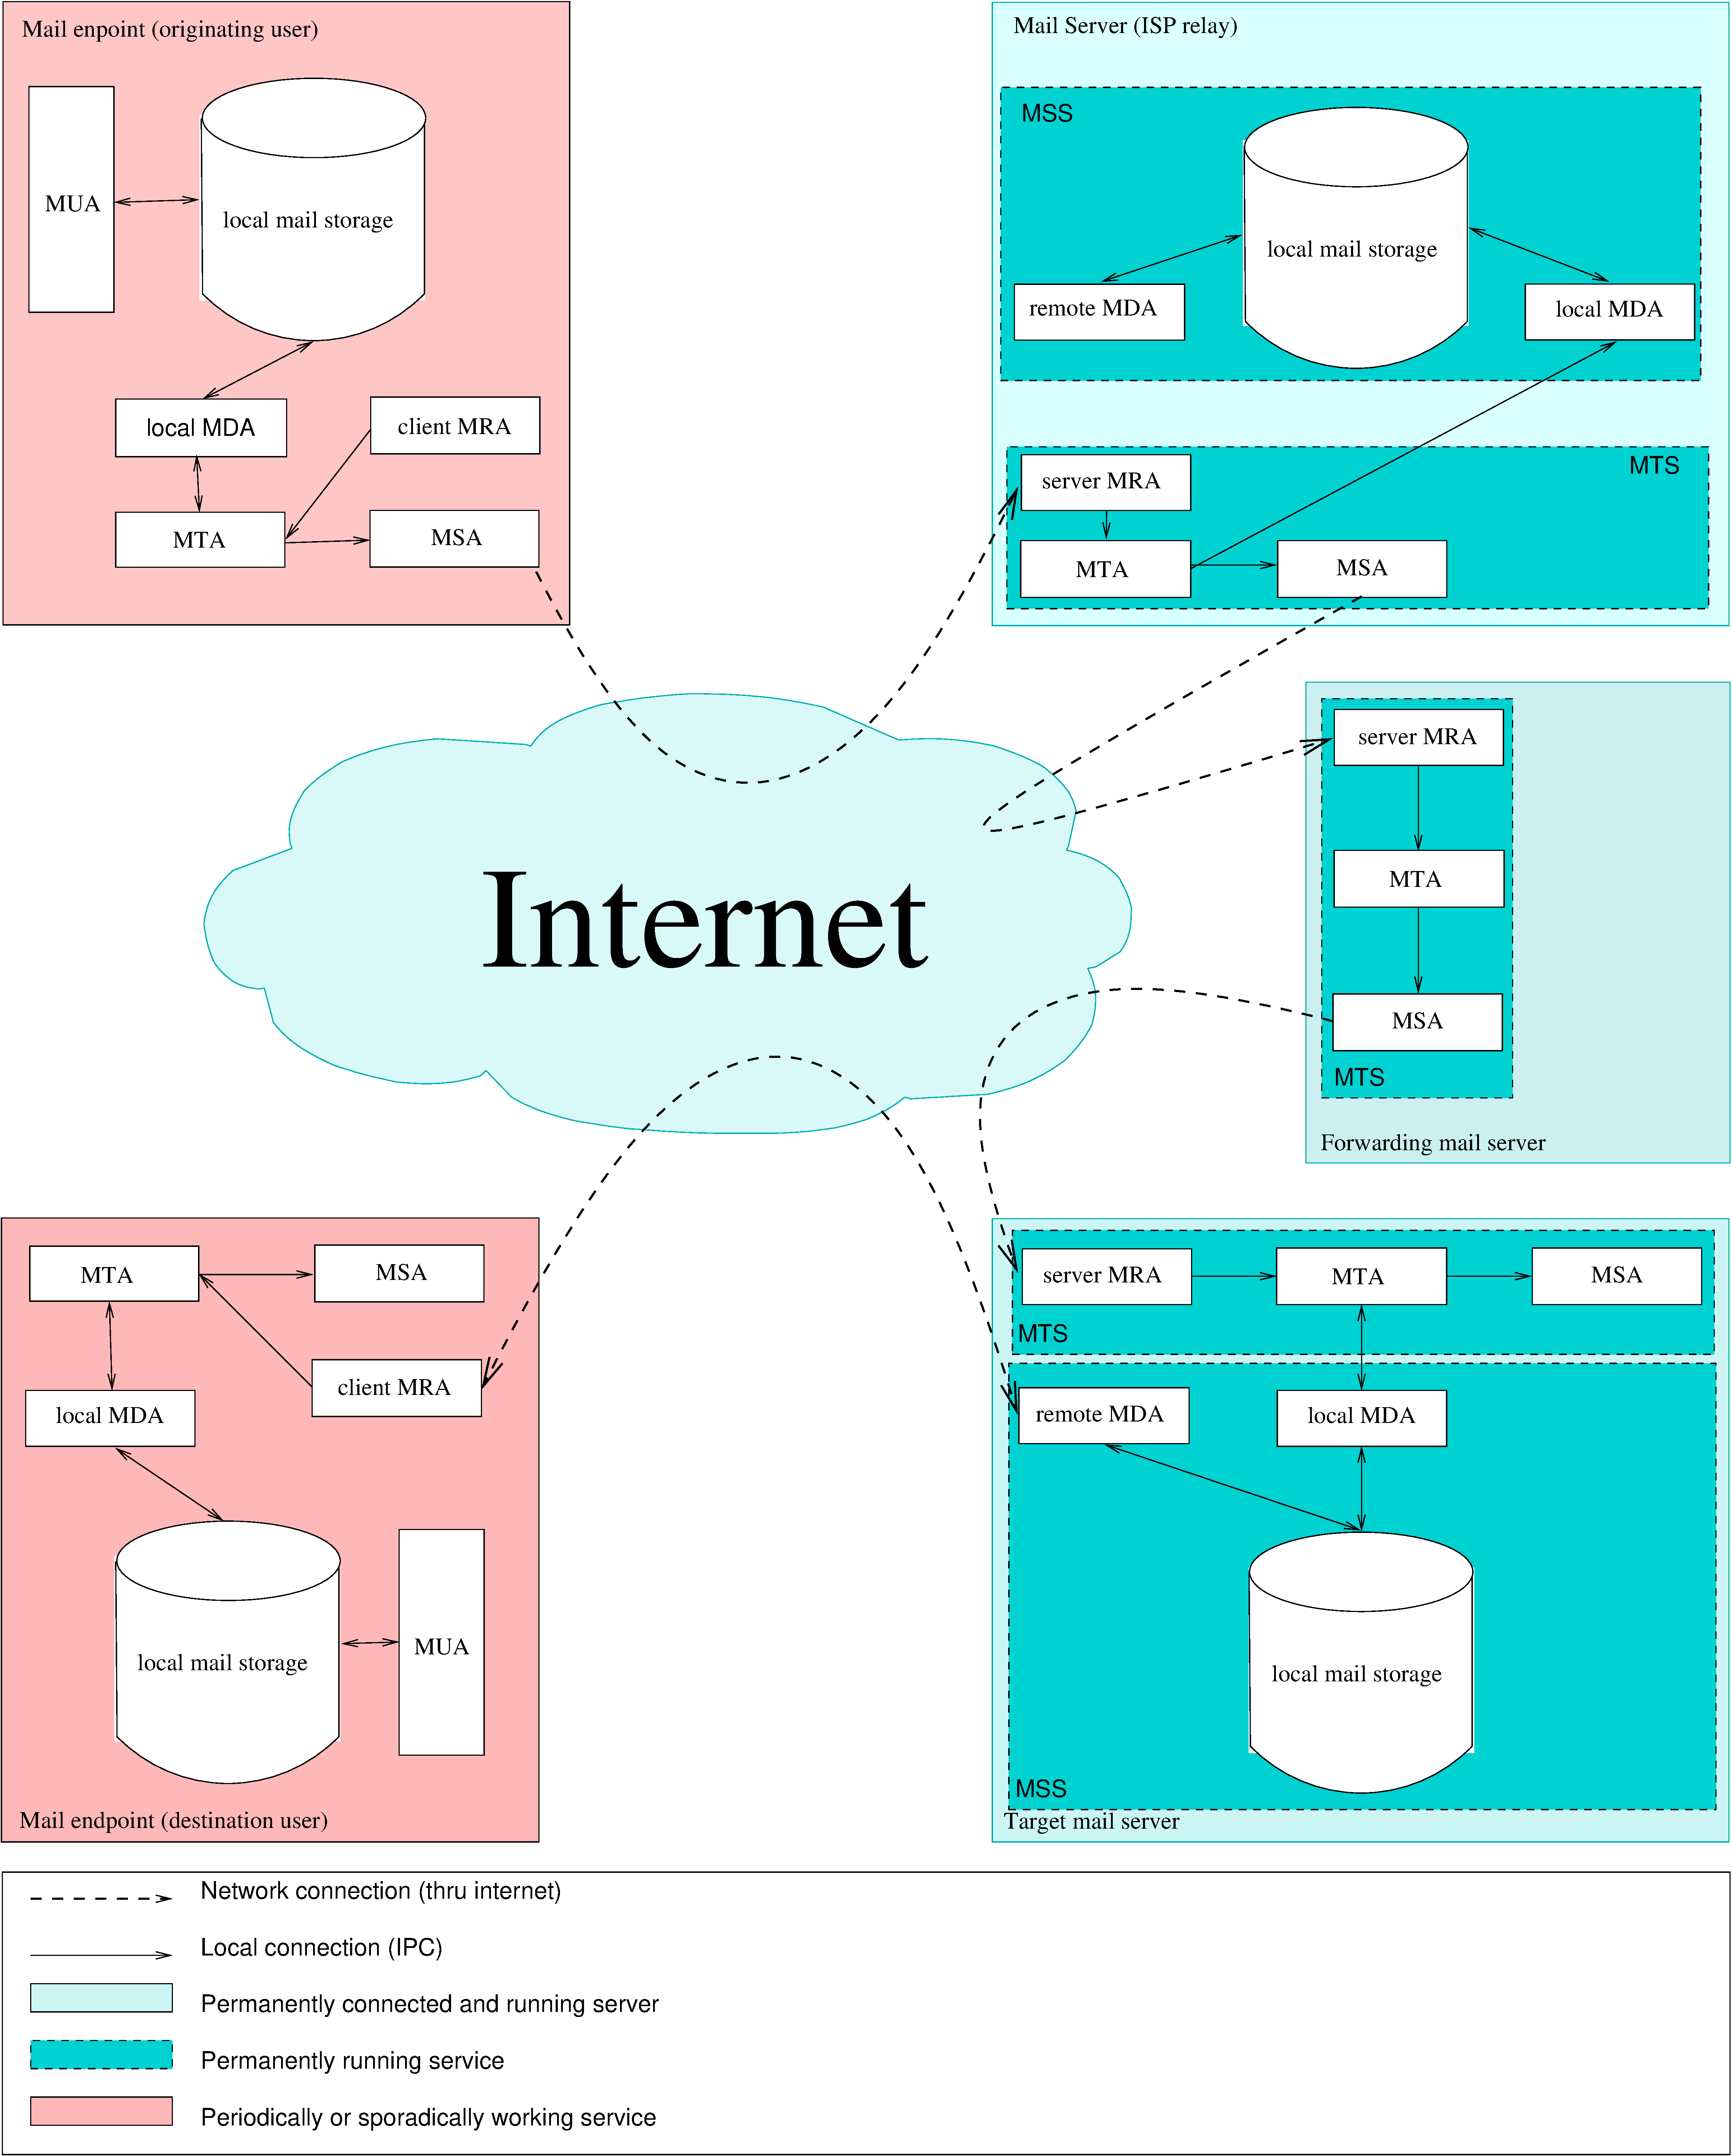
\includegraphics[width=\columnwidth]{inc/MailAgents1.pdf}
	\caption{Mail Agents}\label{fig:MailAgents}
\end{figure}

In the following paragraphs (for definitions), the term ``email'' is used synonymously to the term ``Message''.  ``Email'' has been chosen over ``messages'' because of its frequent use in standard documents.

Emails are typically initiated by a Mail User Agent (\defref{MUA}). An MUA accesses local email storage, which may be the server storage or a local copy. The local copy may be a cache only copy, the only existing storage (when emails are fetched and deleted from the server after retrieval), or a collected representation of multiple server storages (cache or authoritative).

Besides the MUA, the only other component accessing local email storage is the Mail Delivery Agent (\defref{MDA}). An MDA is responsible for storing and fetching emails from the local mail storage. Emails destined for other accounts than the current one are forwarded to the MTA. Emails destined to a User are persistently stored in the local email storage. It is essential to understand that email storage does not necessarily reflect a single mailbox. It may as well represent multiple mailboxes (e.g., a rich client-serving multiple IMAP accounts) or a combined view of multiple accounts (e.g., a rich client collecting mail from multiple \defref{POP} accounts). In the case of a rich client, the local MDA is part of the software provided by the user agent. In the case of an email server, the local MDA is part of the local email store (not necessarily of the mail transport service).

On the server-side, there are usually two components (services) at work. A ``Mail Transport Service'' (\defref{MTS}) responsible for mail transfers and a ``Mail Storage System'' which offers the possibility to store received Mails in a local, persistent store.\par

An MTS generally consists out of three parts. For incoming connects, there is a daemon called Mail Receiving Agent (\defref{Server MRA}) is typically a \defref{SMTP} listening daemon. A Mail Transfer Agent (\defref{MTA}) which is responsible for routing, forwarding, and rewriting emails. Moreover, a Mail Sending Agent (\defref{MSA}) which is responsible for transmitting emails reliably to another Server MRA (usually sent via \defref{SMTP}).\par

An MSS consists of local storage and delivery agents which do offer uniform interfaces to access the local store. They do also deal with replication issues, and grant should take care of the atomicity of transactions committed to the storage. Typically there are two different kinds of \defref{MDA}s. \defref{Local MDA}s offer possibilities to access the store via efficient (non-network based) mechanisms (e.g., IPC or named sockets). This is usually done with a stripped-down protocol (e.g., \defref{LMTP}). For remote agents there a publicly -- network-based -- agent available. Common Protocols for this \defref{Remote MDA}\ include \defref{POP}, \defref{IMAP}, or \defref{MS-OXCMAPIHTTP}.\par

Mail endpoints consist typically of the following components:
\begin{itemize}
	\item A Mail User agent (\defref{MUA})
	\item A Local Mail storage (\defref{MUA})
	\item A Local Mail Delivery Agent (\defref{Local MDA})
	\item A Mail Transfer Agent (\defref{MTA})
	\item A Mail Sending Agent (\defref{MSA})
	\item A Mail Receiving Agent (\defref{MRA})
\end{itemize}

Only two of these components do have external interfaces. These are \defref{MSA} and \defref{MRA}. \defref{MSA} usually uses \defref{SMTP} as transport protocol. When doing so, there are a couple of specialties. 
\begin{itemize}
	\item Port number is 587 (specified in \cite{RFC4409}).\\
	Although port numbers 25 and 465 are valid and do usually have the same capabilities, they are for mail routing between servers only. Mail endpoints should no longer use them.
	\item Connections are authenticated.\\
	Unlike a normal server-to-server (relay or final delivery) SMTP connections on port 25, clients should always be authenticated of some sort. This may be based on data provided by the user (e.g., username/password or certificate) or data identifying the sending system (e.g., IP address)\cite{RFC4409}. Failure in doing authentication may result in this port being misused as a sender for \defref{UBM}.
\end{itemize}

Mail User Agents (MUA) are the terminal endpoint of email delivery. Mail user agents may be implemented as fat clients on a desktop or mobile system or as an interface over a different generic protocol such as HTTP (Web Clients). 

Server located clients are a special breed of fat clients. These clients share the properties of fat clients except for the fact that they do not connect to the server. The client application itself has to be run on the server where the mail storage persists. This makes delivery and communication with the server different. Instead of interfacing with an MSA and a client MDA, they may directly access the local mail storage on the server. On these systems, the local mail storage may be implemented as a database in a user-specific directory structure.

\subsubsection{Fat clients}
The majority of mail clients are fat clients. These clients score over the more centralistic organized web clients in the way that they may offer mail availability even if an Internet connection is not available (through client-specific local mail storage). They furthermore provide the possibility to collect emails from multiple sources and store them in the local storage. Unlike Mail servers, clients are assumed to be not always online. They may be offline most of the time. To guarantee the availability of a particular email address, a responsible mail server for a specific address collects all emails (the \defref{MSS} does this) and provides a consolidated view onto the database when a client connects through a local or remote MDA.

As these clients vary heavily, it is mandatory for the MDA that they are well specified. Lack of doing so would result in massive interoperability problems. Most commonly the Protocols \defref{IMAP}, \defref{POP} and \defref{EWS} are being used these days. For email delivery, the SMTP protocol is used. 

Fat clients are commonly used on mobile devices. According to  \cite{clientDistribution} in Aug 2012 the most typical fat email client was Apple Mail client on iOS devices ($35.6\%$), followed by Outlook ($20.14\%$), and Apple Mail ($11\%$). \citetitle{clientDistribution2}\cite{clientDistribution2} as a more recent source lists in February 2014 iOS devices with $37\%$, followed by Outlook ($13\%$), and  Google Android ($9\%$).

\subsubsection{Server located clients}
Server located clients build an absolute minority. This kind of clients was common in the days of centralized hosts. An example for a Server Located Client is the Unix command ``mail''. This client reads email storage from a file in the users home directory.

\subsubsection{Web clients}
Web clients are these days a common alternative to fat clients. Most big provider companies use their proprietary web client. According to \cite{clientDistribution2} the most common web clients are "`Gmail"', "`Outlook.com"', and "`Yahoo! Mail"'. All these Interfaces do not offer a kind of public plug-in interface. However,  they do offer IMAP-interfaces. This important for a future generalistic approach to the problem.

\subsection{S/MIME}
S/MIME is an extension to the MIME standard. The MIME standard allows in simple text-oriented mails an alternate representation of the same content (e.g., as text and as HTML), or it allows to split a message into multiple parts that may be encoded. It is important to note that MIME encoding is only effective in the body part of a mail.

S/MIME, as described in \cite{RFC3851}, extends this standard with the possibility to encrypt mail content or to sign it. Practically this is achieved by either putting the encrypted part or the signature into an attachment. It is essential to know that this method leaks significant pieces of the data.

As the mail travels directly from sender to recipient, both involved parties are revealed. Neither message subject nor message size or frequency is hidden. This method does offer limited protection when assuming an adversary with interest in the message content only. It does not protect from the kind of adversary in our case. 

The trust model is based on a centralistic approach involving generally trusted root certification authorities.

\subsection{PGP/MIME}
Exactly as S/MIME PGP\cite{rfc4880} builds upon the base of MIME. Although the trust model in PGP is peer-based. The encryption technology does not significantly differ (as seen from the security model).

Like S/MIME, PGP does not offer anonymity. Sender and endpoints are known to all routing nodes. Depending on the version of PGP, some meta-information or parts of the message content such as subject line, the real name of the sender and receiver, message size is leaked.

A good thing to learn from PGP is that peer-based approaches are offering limited possibilities for trust. The trust in PGP is based on the peer review of users. This peer review may give an idea of how well verified the key of a user is.


\section{Pseudo Random Number Generators \label{sec:prng}}
The following sections list two PRNG specifications to follow the recommendations of \cite{rfc1750}. These PRNGs are used to complete the padding specified in the addRedundancy operation.

We have chosen to support two kinds of PRNG. These algorithms are not relevant for the security of the system, but they guarantee non-detectable padding when doing the addRedundancy operation. The two PRNGs selected were xorshift128+ and Blum Micail PRNG. Both PRNGs were quoted to pass BigCrush. However, recent development shows that this might not be true for xorshift128+, as demonstrated in \cite{LEMIRE2019139}.

\section{Known Attacks}
In the following sections, we emphasize on possible attacks to an anonymity preserving protocols. These attacks may be used to attack the anonymity of any entity involved in the message channel. In a later stage, we test the protocol for immunity against these classes of attacks.

\subsection{Broken Encryption Algorithms}
Encryption algorithms may become broken at any time. This either to new findings in attacking them, by more resources being available to an adversary, or by new technologies allowing new kinds of attacks. A proper protocol must be able to react to such threads promptly. This reaction should not rely on a required update of the infrastructure. Users should solely control the grade of security. 

We cannot do a lot for attacks of this kind to happen. However, we might introduce a choice of algorithms, paddings, modes, and key sizes to give the user a choice in the degree of security he wants to have.

\subsection{Attacks Targeting Anonymity}
Attacks targeting users anonymity are the main focus of this work. Many pieces of information may be leaked, and the primary goal should, therefore, rely on the principles established in security.

\begin{itemize}
	\item Prevent an attack\\
	Attack prevention can only be done for attacks that are already known and may not be realistic in all cases. In our protocol, we have strict boundaries defined. A node under attack should at any time of protocol usage (this excepts bandwidth depletion attacks) be able to block malicious identities. Since establishing new identities is costly for an attacker, he should always require far more resources than the defender.
	\item Minimize attack surface\\
	This part of the attack prevention is included by design in the protocol.
	\item Redirect an attack\\
	Although the implementation does not do this, it is possible to handle suspected malicious nodes differently.
	\item Control damage\\
	For us, this means leaving as little information about identities or meta information as possible on untrusted infrastructures. If we leave traces (i.e., message flows, or accounting information) they should have the least possible information content and should expire within a reasonable amount of time.
	\item Discover an attack\\
	The protocol is designed in such a way that attack discovery (such as a query attack) is possible. However, we consider active attacks just as part of the regular message flow. The protocol must mitigate such attacks by design.
	\item Recover from an attack\\
	An attack does always impose a load onto a system's resources regardless of its success. It is vital that a system recovers almost immediately from an attack and is not covered in a non-functional or only partial-functional state either temporarily or permanently.
\end{itemize}

In the following subsections, we list a couple of attack classes that have been used against systems listed in \ref{sec:sysImpl} or the respective academic works. We list the countermeasures which have been taken to deflect these attacks.

\subsubsection{Probing Attacks}
Identifying a node by probing and check their reaction is commonly done when fingerprinting a service. As a node is participating in a network and relaying messages probing may not be evaded. However, it may be made costly for an adversary to do systematic probing. This should be taken into account. Both currently specified transport protocol features an indefinite number of possible accounts. Since not the server but the endpoint address is behaving, node probing is more complicated than in other cases where probing of service is sufficient. 

One of the problems is clear-text requests. These requests may be used on any transport layer account without previous knowledge of any host key. Thus the recommendation in table \ref{tab:protoReplyCrit} is generally not to answer the requests. Routing nodes in jurisdictions not fearing legal repression or prosecution may reply to clear text requests, but it is usually discouraged as they allow harvesting of addresses.

One strategy to avoid would be to put high costs onto clear-text requests in such a way that a clear-text request may have a long reply time (e.g., up to one day). A node is free to blacklist an identity in case of an early reply. This is an insufficient strategy as a big adversary may have lots of identities in stock. Requesting an unusually long key as a plain-text identity does not make sense either as these as well may be kept in stock. We may, however, force a plaintext request to have an identity block with a hash following specific rules. We may, for example, put in a requirement that the first four bytes of the hash of a header block translates to the first four characters of the routing block. At the moment, this has been rejected in the standard for practical reasons. First, as the request is unsolicited, a sender is the only one able to decide the algorithm of the hash. This would allow a requester to choose upon the complexity of the puzzle. Second, any negotiation of the cost of the request would result in the disclosure of the node as VortexNode, which might be unsuitable.

\subsubsection{Hotspot Attacks}
Hotspot attacks aim to isolate high traffic sites within a network. By analyzing specific properties or the general throughput locations with outstanding traffic may be identified. These messages do quite often reveal senders or recipients. Sometimes an intermediate node in an anonymizing system. 

\subsubsection{Message Tagging and Tracing}
When using an anonymization system, a message may be either fully or partially traced or even tagged. Tagging allows one to recognize a message at a later stage and map it to its predecessors. Protocols with tagable messages are not suitable for anonymization systems.

\subsubsection{Side Channel Attacks}
Side-channel attacks are numerous. Especially important to us are attacks related to either lookup in independent channels (e.g., downloading of auxiliary content of a message) or behavior related to timing patterns.

\subsubsection{Sizing Attacks}
There are two kinds of sizing attacks identified to be relevant for us. One is the possibility for matching messages with related sizes, and the other one is to relate message size to the original messages. Both attacks may be considered as a tracing attack and will be analyzed accordingly.

\subsubsection{Bugging Attacks}
Numerous attacks are available through the bugging of a protocol. In this chapter, we outline some of the possibilities and how they may be countered:

\begin{itemize}
	\item Bugging through certificate or identity lookup:\\
	Almost all kinds of proof of identities, such as certificates, offer some revocation facility. While this is a perfect desirable property of these infrastructures, they offer a flaw. Since the location of this revocation information is typically embedded in the proof of identity, an evil attacker might use a falsified proof of identity with a recording revocation point.
	
	There are multiple possibilities to counter such an attack. The easiest one is to do no verification at all. Having no verification is, however, not desirable from the security point of view. Another possibility is only to verify trusted proof of identities. By doing so, the only attacker could be someone having access to a trusted source of proof of identities. A third possibility is to relay the request to another host either by using an anonymity structure such as Tor or by using its infrastructure. Using Tor would violate the ``Zero Trust'' goal. Such a measure would only conceal the source of the verification. It would not hide the fact that the message is processed. A fourth and most promising technology would be to force the sender of the certificate to include a ``proof of non-revocation''. Such a proof could be a timestamped and signed partial CRL. It would allow a node to verify the validity of a certificate without being forced to disclose itself by doing a verification. On the downside has to be mentioned that including proof of non-revocation involves the requirement to accept a certain amount of caching time to be accepted. This allowed caching time reduces the value of the proof as it may be expired in the meantime. It is recommended to keep the maximum cache time as low as 1d to avoid that revoked certificates may be used. 
	
	\item Bugging through DNS traffic:\\
	A standard protocol on the Internet is DNS. Almost all network-related programs use it without thinking. Typically the use of such protocol is only a minor issue since the resolution of a lookup usually done by an ISP. In the case of a small Internet service provider (ISP), this might, however, already become a problem.
	
	The bugging in general attack works as follows: We include a unique DNS name to be resolved by a recipient. This can be done most easily by adding an external resource such as an image. A recipient will process this resource and might, therefore, deliver information about the frequency of reading, or the type of client. 
	
	It must be taken into account that the transport layer will always do DNS lookups and that we may not avoid this attack completely. We may, however, minimize the possibilities of this attack.
	
	\item Bugging through external resources:\\
	A straightforward attack is always to include external resources into a message and wait until they are fetched. In order to avoid this kind of attack, plain text or other self-contained formats should be used when sending a message. As we may not govern the type of contained message, we can make at least recommendations concerning its structure.
\end{itemize}

\subsection{Denial of Service Attacks}
\subsubsection{Censorship}
Whereas traditional censorship is widely regarded as selective information filtering and alteration, very repressive censorship can even include denial of information flows in general. Any anonymity system not offering the possibility to hide in legitimate information flows, therefore not censorship-resistant.

\subsubsection{Denial of service}
An adversary may flood the system in two ways.
\begin{itemize}
	\item He may flood the transport layer exhausting resources of the transport system.\\
	This is a straightforward attack. MessageVortex has no control over the existing transport protocol. Therefore, all flooding attacks on that layer are still effective. However, If an adversary attacks a node, the redundancy of a message may still be sufficient. On the other hand, flooding disrupts at least all other services using the same transport layer on that node. This result may be unacceptable for an attacker. More likely would be censorship.
	\item He may flood the routing layer with invalid messages.\\ 
	Identifying the messages is relatively easy for a node. Usually, it should be sufficient to decode the CPREFIX block of a message. If the CPREFIX is valid, then the header block either identifies a valid identity or processing may be aborted. 
	\item He may flood an accounting layer with newIdentity.\\
	Flooding an accounting layer with identities is possible. Since the accounting layer is capable of adapting costs to a new identity, it may counter this attack by giving large puzzles to new identities. This affects all new identities and not only those flooding. If a flooding attack is carried out over a long time, a node may decide to split its identity. All recent active users get a new identity, whereas the old one opposes high costs. This would force an attacker to work in intervals and is no longer able to make a permanent DoS attack.
\end{itemize}

\subsubsection{Credibility Attack}
Another type of DoS attack is the credibility attack. While not a technical attack, it is very effective. A system not having a sufficiently big user base is offering thus a lousy level of anonymity because the anonymity set is too small or the traffic concealing message flow is insufficient. 

Another way is to attack the reputation of a system in such a way that the system is no longer used. An adversary has many options to achieve such a reduction in credibility. Examples:
\begin{itemize}
	\item Disrupt functionality of a system.\\ 
	This may be done by blocking of the messaging protocol it uses or by blocking messages. Furthermore, an adversary reduces functionality when removing known participants from the network either by law or by threatening.
	\item Publicly dispute the effectiveness of a system.\\
	Disputing the effectiveness is a very effective way to destroy a system. People are not willing to use a system which believed to be compromised if the primary goal of using the system is avoiding being observed.
	\item Reduce the effectiveness of a system.\\
	A system may be considerably loaded by an adversary to decrease the positive reception of the system. He may further use the system to send \defref{UBM} to reduce the overall experience when using the system. Another way of reducing effectiveness is to misuse the system for evil purposes such as blackmailing and making them public.
	\item Dispute the credibility of the system founders.\\
	Another way of reducing the credibility of a system is to undermine its creators. If -- for example -- people believe that a founders' interest was to create a honey pot (e.g., because he is working for a potential state-sponsored adversary) for personal secrets, they will not be willing to use it.
	\item Dispute the credibility of the infrastructure.\\
	If the infrastructure is known or suspected to be run by a potential adversary, people's willingness to believe in such a system is expected to be drastically reduced.
\end{itemize}

\chapter{Applied Methodes\label{sec:appliedMethods}}
Based on the findings of the previous chapter, we used the following methodology in order to find a solution:
\begin{enumerate}
	\item Identify problem hotspots for a new protocol.
	\item Design a protocol that addresses the previously identified hotspots.
	\item Build a protocol prototype.
	\item Analyse the protocol for weaknesses using attack schemes.
	\begin{enumerate}
		\item Tagging/Bugging attacks.
		\item Tracing attacks.
		\item Content and identification targeting attacks.
		\item DoS attacks.
	\end{enumerate}
\end{enumerate}

\section{Problem Hotspots}
Starting from the previous research, we identified several hotspots that have to be taken care of. The following sections list identified problems and the possible countermeasures which have not been broken in the past.

\subsection{Zero Trust Philosophy}
One main disadvantage of almost any system listed in section \ref{sec:sysImpl} is that trust (unlimited or limited) has been put into the infrastructure. For example, when using ToR, we need to trust the directory servers. Control over the directory servers might give an attacker the possibility to redirect a connection to controlled entry and exit nodes, which would then break anonymity. In general, control of entry and exit nodes makes a system vulnerable. 

To avoid this problem, we decided to apply a zero trust model. We do not trust any platform except for the sending and the receiving computer. We assume that all other devices may be compromised and do create detailed logs about what they are doing. This trust extends partially to our personally known contacts. We believe that some of them might be evil, but they are generally trustworthy. We furthermore assume that traffic on the network layer is observed and recorded at any time. This philosophy creates very hard to meet goals. However, by assuming so, we prevent the system from leaking information through side channels.

\begin{requirement}{zeroTrust}{Zero Trust}
	No infrastructure should be trusted unless it is the senders' or the recipients' infrastructure.
\end{requirement}    

\subsection{Information leakage and P2P Design}
An anonymizing system must keep information on messages or their metadata within the system. Ideally, even not disclosing to its members. In a perfectly encrypted system, such metadata is leaked at least by the entry and the exit node. To avoid this, all peers must behave alike. All nodes should be valid endpoints as well as legitimate senders or mixes. Covering all functions in all nodes implies a design with equally built nodes and is shared with many P2P designs.

A fundamental problem of the P2P design is that usually, port forwarding or central infrastructure is required. Technologies such as ``hole punching'' and ``hairpin translation'' typically require central infrastructures to support at least the connection and maybe depending on the client infrastructure being used fragile or ineffective. To avoid these problems we decided to rely on traditional centralistic transport infrastructures. As proof of concept, we decided to use SMTP. 

The approach supports, however, even mixing transport media. This makes it harder for an attacker to trace a message as the message flow may go through any suitable transport protocol at any time of message transfer.

\begin{requirement}{P2P}{Equal nodes}
	Mixes and peers must be indistinguishable from each other. 
\end{requirement}

To guarantee that information is not leaked through owners of systems or to protect such owners from being forced into cooperation, the system needs to be undetectable.
\begin{requirement}{undetectable}{Undetectable}
	Nodes should be undistinguishable from regular transport media traffic. 
\end{requirement}

\subsubsection{Decoy traffic generation}
To create decoy traffic in an untrusted way, we need means to increase and decrease messages in size without knowledge of the routing node. A straightforward approach would be to create decoy traffic in the initial message. Such a design would create a pattern of decreasing or repeating message sizes in the net. To avoid this, we introduced a set of operations to be applied to the original message. The operations are done in such a way that a mixer is unable to tell whether the message size or decrease results in decoy traffic generation/removal or not.

The main message operations are:
\begin{itemize}
	\item Split and merge messages.
	\item Add and remove redundancy information.
	\item Encrypt and Decrypt information.
\end{itemize}

At this point, we could have used homomorphic encryption instead of redundancy operations. Such encryption would, however, add much complexity to the algorithm with no apparent gain.

\subsubsection{Message tagging or bugging protection}
It is essential to the protocol that any operation at any point of the protocol handling, which is not foreseen, should fail in message transport. This property makes the protocol very fragile, but it prevents mixes from introducing tags which may be followed throughout the system. The protocols counter this fragility by the fact that redundancy added in the message course may be used to recover from misbehaving nodes.

In our approach, we give a single mix called the routing block builder (RBB) full control over the message transport layer. The content used for blending is discardable data. RBB has no control over this aspect. This blending data is ephemeral and will (or may) be removed by the next node. The data received by a mix may be used to generate a ``pseudo reply'' on the blending layer to transport any other message (related or unrelated) back to the sending node. So tagging on this layer is worthless.

The reason for not giving control over the behavior to this layer to the sender of the message is simple. By giving him control over it, we would allow him to use the information provided here as the primary medium. As an immediate result, the system would be suitable to blackmail any user of the world. It furthermore would create unintentional ``exit nodes'' to the system, which might oppose further legal threads for participants.

\begin{requirement}{untagable}{untagable}
	The message should be un-tagable (neither by a sender nor by an intermediate party such as a mixer).
\end{requirement}

\begin{requirement}{unbugable}{unbugable}
	The message should be unbugable (neither by the sender nor by an intermediate party such as a mixer).
\end{requirement}

\subsubsection{Message replay protection}
Message reply protection is crucial for such a system. With the ability to replay a message, an adversary may ``highlight'' a message flow as it would always generate the same traffic pattern. So there needs to be a reply pattern protecting the protocol from message replay. As we do have MURBs in our protocol, this is a problem. A MURB is by design replayable. We, therefore, need a possibility for the original sender using a MURB to make messages distinguishable, which may not be used by an adversary.

\begin{requirement}{replay}{replay}
	A message must not be replayable.
\end{requirement}

It should be able to increase and shrink in size, or all messages must have a uniform size. Decoy traffic should not be distinguishable from message traffic. 

\subsubsection{No Dedicated Infrastructure Philosophy}
There should be no infrastructure dedicated to the operation of the solution. This avoids a single point of failure, as well as the possibility for an adversary to shut down this infrastructure to disrupt the functioning of the system as a whole. This requirement is already covered implicitly in \ref{req:zeroTrust}.

\subsection{Accounting}
The infrastructure must not be misused as \defref{UBM} sending infrastructure. This implies that sending messages is connected to some ``cost''. ``Costs'' must be connected to some identity to allow accounting. Linking to a global identity would allow assigning traffic to a real-world user. Therefore the protocol must allow creating ephemeral local identities not linked to a real identity.

\begin{requirement}{accounting}{accounting}
	The system must be able to do accounting without being linked to a real identity.
\end{requirement}

\subsection{Anonymisation}
The system must allow the anonymizing of message source and message destination at any point. It should not be visible to the infrastructure protocol whether a message has reached its destination or not. 

\begin{requirement}{anon}{anonymisation}
	A system must be able to anonymize sender and recipient at any point of the transport layer and any point of mixing unless it is the sender or the recipient itself.
\end{requirement}

\subsection{Initial Bootstraping}
The system must allow bootstrapping from a zero-knowledge or near-zero knowledge point. Therefore, the protocol must be able to extend the network of known nodes on its own.

\begin{requirement}{boot}{bootstrapping}
	The system must allow to bootstrap from a zero-knowledge or near-zero-knowledge point and extend the network on its own. 
\end{requirement}

\subsection{Cypher selection}
In this protocol, a lot of encryption and hashing algorithms have to be used. This choice of these algorithms should be explained. 

From the requirements side, we have to follow the following principle:
\begin{requirement}{algVar}{algorithmic variety}
	The system must be able to use multiple symmetric, asymmetric, and hashing algorithms to immediately fall back to a secure algorithm for all new messages if required. 
\end{requirement}

First of all, we need a subset of encryption algorithms all implementations may rely on. Defining such a subset guarantees interoperability between all nodes regardless of their origins. 

Secondly, we need to have a spectrum of algorithm in such a manner that it may be (a) enlarged if necessary and (b) there is an alternative if an algorithm (or a mathematical problem class) is broken (so that algorithms may be withdrawn if required without affecting the function in general). 

And third, due to the onion-like design described in this document, asymmetric encryption should be avoided in favor of symmetric encryption to minimize losses due to the key length and the generally higher CPU load opposed by asymmetric keys.

If the algorithm is generally bound to specific key sizes (due to S-Boxes or similar constructs), the key size is incorporated into the definition. If not, the key size is handled as a parameter.

The key sizes have been chosen in such a manner that the key types form tuples of approximately equal strength. The support of Camelia192 and Aes192 has been defined as optional. However, as they are wildly common in implementations, they have already been standardized as they build a possibility to step up security in the future.

Having these criteria for choice, we chose to use the following keys and key sizes:
\begin{itemize}
	\item Symmetric
	\begin{itemize}
		\item AES (key sizes: 128, 192, 256)
		\item Camellia (key sizes: 128, 192, and 256)
	\end{itemize}
	\item Asymmetric
	\begin{itemize}
		\item RSA (key size: 2048, 4096, and 8192)
		\item Named Elliptic Curves
		\begin{itemize}
			\item secp384r1
			\item sect409k1
			\item secp521r1
		\end{itemize}
	\end{itemize}
	\item Hashing
	\begin{itemize}
		\item sha3-256
		\item sha3-384
		\item sha3-512
		\item RIPE-MD160
		\item RIPE-MD256
		\item RIPE-MD320
	\end{itemize}
\end{itemize}

Within the implementation, we assigned algorithms to a security strength level:
\begin{itemize}
	\item LOW\\
	AES128, Camellia128, RSA1024, sha3-256
	\item MEDIUM\\
	AES192, Camellia 192, RSA2048, ECC secp384r1, sha3-256
	\item HIGH\\
	AES256, Camellia256, RSA4096, ECC sect409k1, sha3-384
	\item QUANTUM\\
	AES256, Camellia256, RSA8192, ECC secp521r1, ntru, sha3-512
\end{itemize}

This allows categorizing the used algorithms to a strength. This list, however, should only serve the purpose of selecting algorithms for people without cryptological know-how.

\subsection{Reed-Solomon function}
Originally \cite{reed1960polynomial} introduced a system allowing the use of polynomial codes to create error-correcting codes. In \cite{chaum1988multiparty} \citeauthor{chaum1988multiparty}, they have shown that the codes are suitable for distributing data assuming enough parties are honest.

Unlike Chaum et al.'s proposition, we are not using the Reed Solomon function to achieve anonymity or privacy. Instead, we use it for decoy traffic generation. We are splitting a message into multiple parts at several points when routing and assemble it again on different nodes. By doing so, we achieve two vital things. First, we introduce the possibility of recovering errors due to misbehaving nodes, and secondly, the real traffic can no longer be differentiated from decoy traffic. 

\subsection{Usability}
The system must be usable without cryptographic know-how and with popular tools. This is necessary to accept the system broadly and makes it easy to use for peoples already communicating.

\begin{requirement}{easy}{easy handleable}
	The system must be usable without cryptographic know-how and with popular tools.
\end{requirement}

\section{Protocol outline}
The protocol itself is independent of the transport layer specified. We emphasize in this section to the general building blocks, the cryptographic structure, and the general protocol attributes. In section \ref{sec:spec}, we will then further elaborate on the protocols' inner structure.

The protocol is built on multiple layers. On the logic side, the protocol is split into two parts:
\begin{enumerate}
	\item Transport Layer\\
	Standard Internet infrastructures provide this Layer. The primary goal is to hide or blend our protocol into regular traffic within that layer.
	\item Blending and subsequent layers\\
	Any user of the Internet may provide these layers. Since these layers may be mixes-only, or valid endpoints. Mixes may or may not be publicly known. In a first implementation, we build this system as a standard Java application. The primary goal is to compile it to native code afterward and run it on an SoC like infrastructure such as a RaspberryPi or port it to an android device.
	
	We may further split these layers into
	\begin{enumerate}
		\item Blending layer\\
		This layer takes messages and creates transport layer conformant messages. In an ideal case, the messages generated by this layer are indistinguishable from the regular message traffic, and the embedded message is only visible for the receiving node.
		\item Routing layer\\
		The routing layer disassembles and reassembles messages. This operation guarantees that messages are generated in such a way that decoy traffic is not differentiable from non-decoy traffic.
		\item Accounting layer\\
		The accounting layer has three jobs. First, he has to authorize the message processing after decrypting the header block. Secondly, he handles all header request blocks and the reply blocks. And third, it keeps track of the accounting regarding the sent messages.    
	\end{enumerate}
\end{enumerate}

%%%%%%%%%%%%%%%%%%%%%%%%%%%%%%%%%%%%%%%%%%%%%%%%%%%%%%%%%%%%%%%%%%%%%%%%%%%%%%%%%%%%%%%
% revise from this point on %%%%%%%%%%%%%%%%%%%%%%%%%%%%%%%%%%%%%%%%%%%%%%%%%%%%%%%%%%%
%%%%%%%%%%%%%%%%%%%%%%%%%%%%%%%%%%%%%%%%%%%%%%%%%%%%%%%%%%%%%%%%%%%%%%%%%%%%%%%%%%%%%%%

\subsection{Protocol Terminology}
For our protocol, we use the following terms:
\begin{itemize}
	\item \textbf{Sender:} The user or process originally composing the message.
	\item \textbf{Recipient:} The user or process destined to receive the message in the end.
	\item \textbf{Router:} Any node which is processing the message. Please note that all nodes are routers.
	\item \textbf{Message:} The ``real content'' to be transferred from the sender to the recipient.
	\item \textbf{Payload:} Any data transported between routers regardless of the meaningfulness or relevance to the message.
	\item \textbf{Decoy traffic:} Any data transported between routers that have no relevance to the message at the final destination.
	\item \textbf{Identity:} A tuple of a routable address, and a public key. This tuple is a long-living tuple but may be exchanged from time to time. 
	\item \textbf{Ephemeral Identity:} An identity created on any node with a limited lifetime anyone possessing the private key (proven by encrypting with it) is accepted as representative of that identity.
	\item \textbf{Routing Block Builder (RBB):} An entity, which is building a routing block. Typically identical to either sender or receiver.
\end{itemize}

\subsection{Vortex Communication model}
In this section, we introduce a new consistent, transport-independent model for representing the different protocols used by MessageVortex.

\begin{figure}[ht!]
	\centering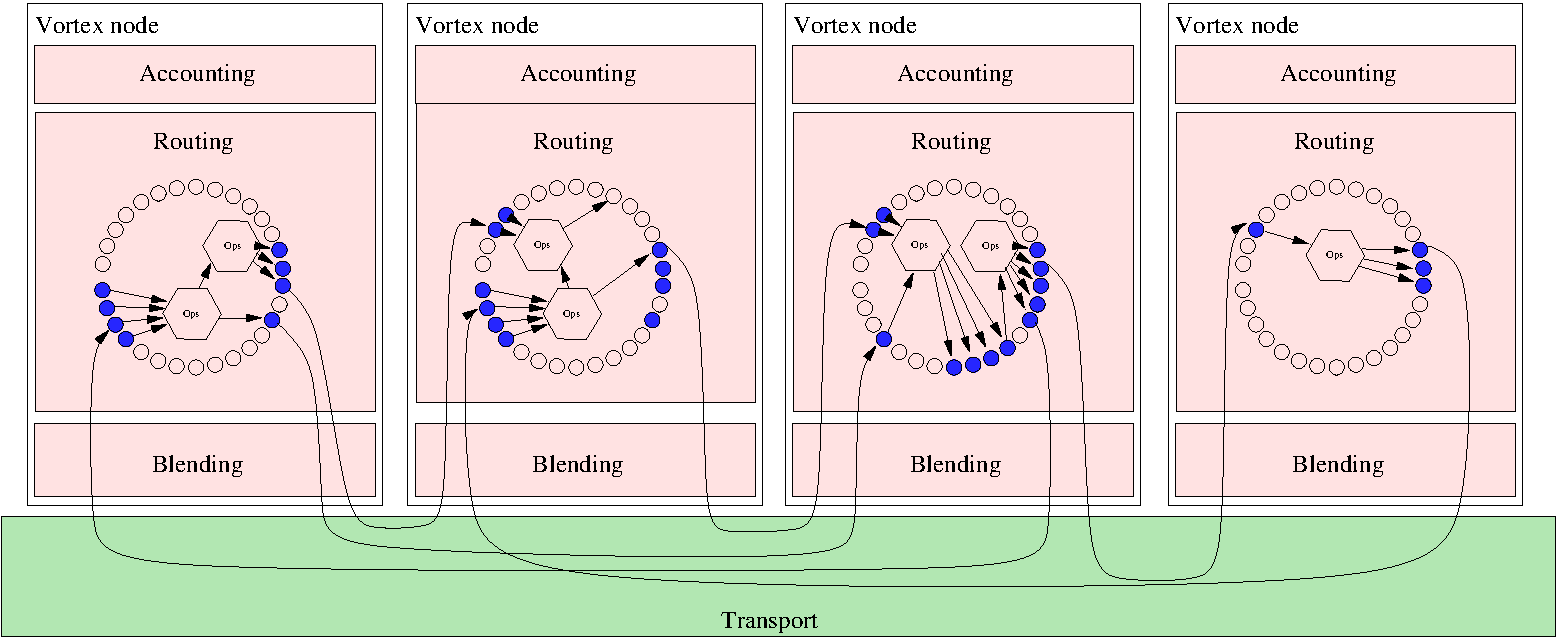
\includegraphics[width=\columnwidth]{inc/roughProtocolDesign.pdf}
	\caption{A rough protocol outline of the MessageVortex protocol}\label{fig:protocolOutline}
\end{figure}

We divide our protocol into four different layers, whereas only three are specific to the MessageVortex protocol. The lowest layer is the transport layer. As expressed earlier, dedicated protocols are easy to censor. Therefore we build our protocol on top of other suitable transport protocols. 

The other Three layers are vortex specific and do not require any infrastructure on the Internet. We elaborate further on these layers in the next section.

\subsection{Transport Layer}
For our first tests, we used a custom transport layer, allowing us to monitor all traffic quickly, and build structures in a very flexible way. This transport layer works locally with a minimum amount of work for setup and deployment. It furthermore works across multiple hosts in a broadcast domain. The API may be used to support almost any kind of transport layer.

After that, we focussed on the protocols identified in the previous sections for transport:
\begin{itemize}
	\item \defref{SMTP}
	\item \defref{XMPP}
\end{itemize}
For the prototype, we have implemented an SMTP transport agent and the respective blending layer.

\subsection{Blending Layer\label{sec:blending}}
The blending layer is taking care of multiple problems:
\begin{itemize}
	\item It is translating the message block into a suitable format for transport\\
	This translation includes jobs such as embedding a block as encoded text, as a binary attachment or hide it within a message using steganography.
	\item Extract incoming blocks\\
	Identify incoming messages containing a possible block and extract it from the message.
	\item Do housekeeping on the storage layer of the transport protocol\\
	Access protocols POP and IMAP require that messages are deleted from time to time to stay below the sizing quotas of an account.      
\end{itemize}

We define the blending layer to work as follows when receiving messages:

\begin{enumerate}
	\item Log arrival time (in UTC) on the transport layer.
	\item Extract possible blocks.
	\item Apply decryption on a suspected header block.
	\item Identify the header block as valid by querying the accounting.
	\item Extract and decrypt subsequent blocks.
	\item Pass extracted blocks and information to the routing layer.
\end{enumerate}

We define the blending layer to work as follows for sending messages:

\begin{enumerate}
	\item Assemble message as passed on by the routing layer.
	\item Using the blending method specified in the routing block, build an empty message. 
	\item Create a message decoy content.
	\item Send the message to the appropriate recipient using the transport layer protocol.
\end{enumerate}

There is no specification on the housekeeping part of the blending layer, as this part is specific to the requirements of the account owner. We do, however, recommend to handle messages precisely as if the messages would be handled on an account handled by a human. 

\subsection{Routing Layer\label{sec:routing}}
The routing layer receives the message blocks in a decrypted and authorized form from the blending layer and processes them as follows:

\begin{itemize}
	\item Build structure representing the block building and the appropriate block IDs.
	\item Schedule all Routing blocks for processing in a priority queue.
	\item Authorise all routing blocks ready for processing with the calculated block sizes.
	\item Process blocks.
	\item Send prepared building blocks to the Blending layer.
\end{itemize}

\subsubsection{Block Structure}
A VortexMessages' main block structure is a sequence of blocks. This block sequence starts with a header containing a symmetric key encrypted with the public key of the current node and a header block containing the immediate details to decrypt the subsequent blocks (if any).

A routing block follows the header block. This routing block contains the information required for subsequent routing. According to the instructions in this block, valid data blocks may be processed, assembled, and sent to a subsequent location. 

The next block is the routing log block. This block protocols the routing information of a message and is somewhat similar to an onionized variant of the received headers in SMTP.

The last part of the message is a sequence of data blocks. They contain the actual data or decoy traffic.

\subsubsection{MURBs\label{sec:murb}}
The protocol includes the capability of MURBs. Such MURBs enable a user to send a limited amount of times messages to an anonymous receiver. Such sending may be done without having any knowledge about its identity, the location, or infrastructure he is using.

A MURB in our term is an entirely prepared routing instruction built by the recipient of a message. The sender has only the routing blocks and the instructions to assemble the initial message. It does not know the message path except for the first message hops.

As a MURB is a routing block, it generates the same pattern on the network each time a sender uses it. To avoid statistical visibility, we need to limit the number of uses per MURB. As a maximum number of usages, the protocol is limited to 127 usages. This number should be sufficiently sized for automated messages. A minute pattern would disappear after 2 hours latest and an hourly pattern after five days.

For a MURB to work, the RBB has to take care that all quotas required to the route are sufficiently sized. Such sizing is hard to foresee in some cases. An RBB may query these identities from time to time to make sure that they do not deplete. Wherever possible, MURBs should be dropped in favor of multiple SURBs to avoid the dangers of MURBs.

\section{Protocol handling}
In the following sections, we outline the handling of messages we split the handling into incoming messages and outgoing messages. All handling assumes that we have a blending layer independently picking up messages as advertised in the capabilities messages.

\subsection{Block Processing}
A Block is picked up in the blending layer and then handled in the routing layer. First, we try to authenticate the message. If we can authenticate the message, we process it and add the contained instructions to a processing workspace. Unauthenticated messages may be discarded at any point.

The processing of a sending block is triggered by a routing block in the workspace, as shown in figure~\ref{fig:msgSendProcessing}. The assembly instructions are processed to collect the payload blocks. Then the encryption is applied to the message and passed on to the blending layer for processing.

\begin{figure*}[hbt]
	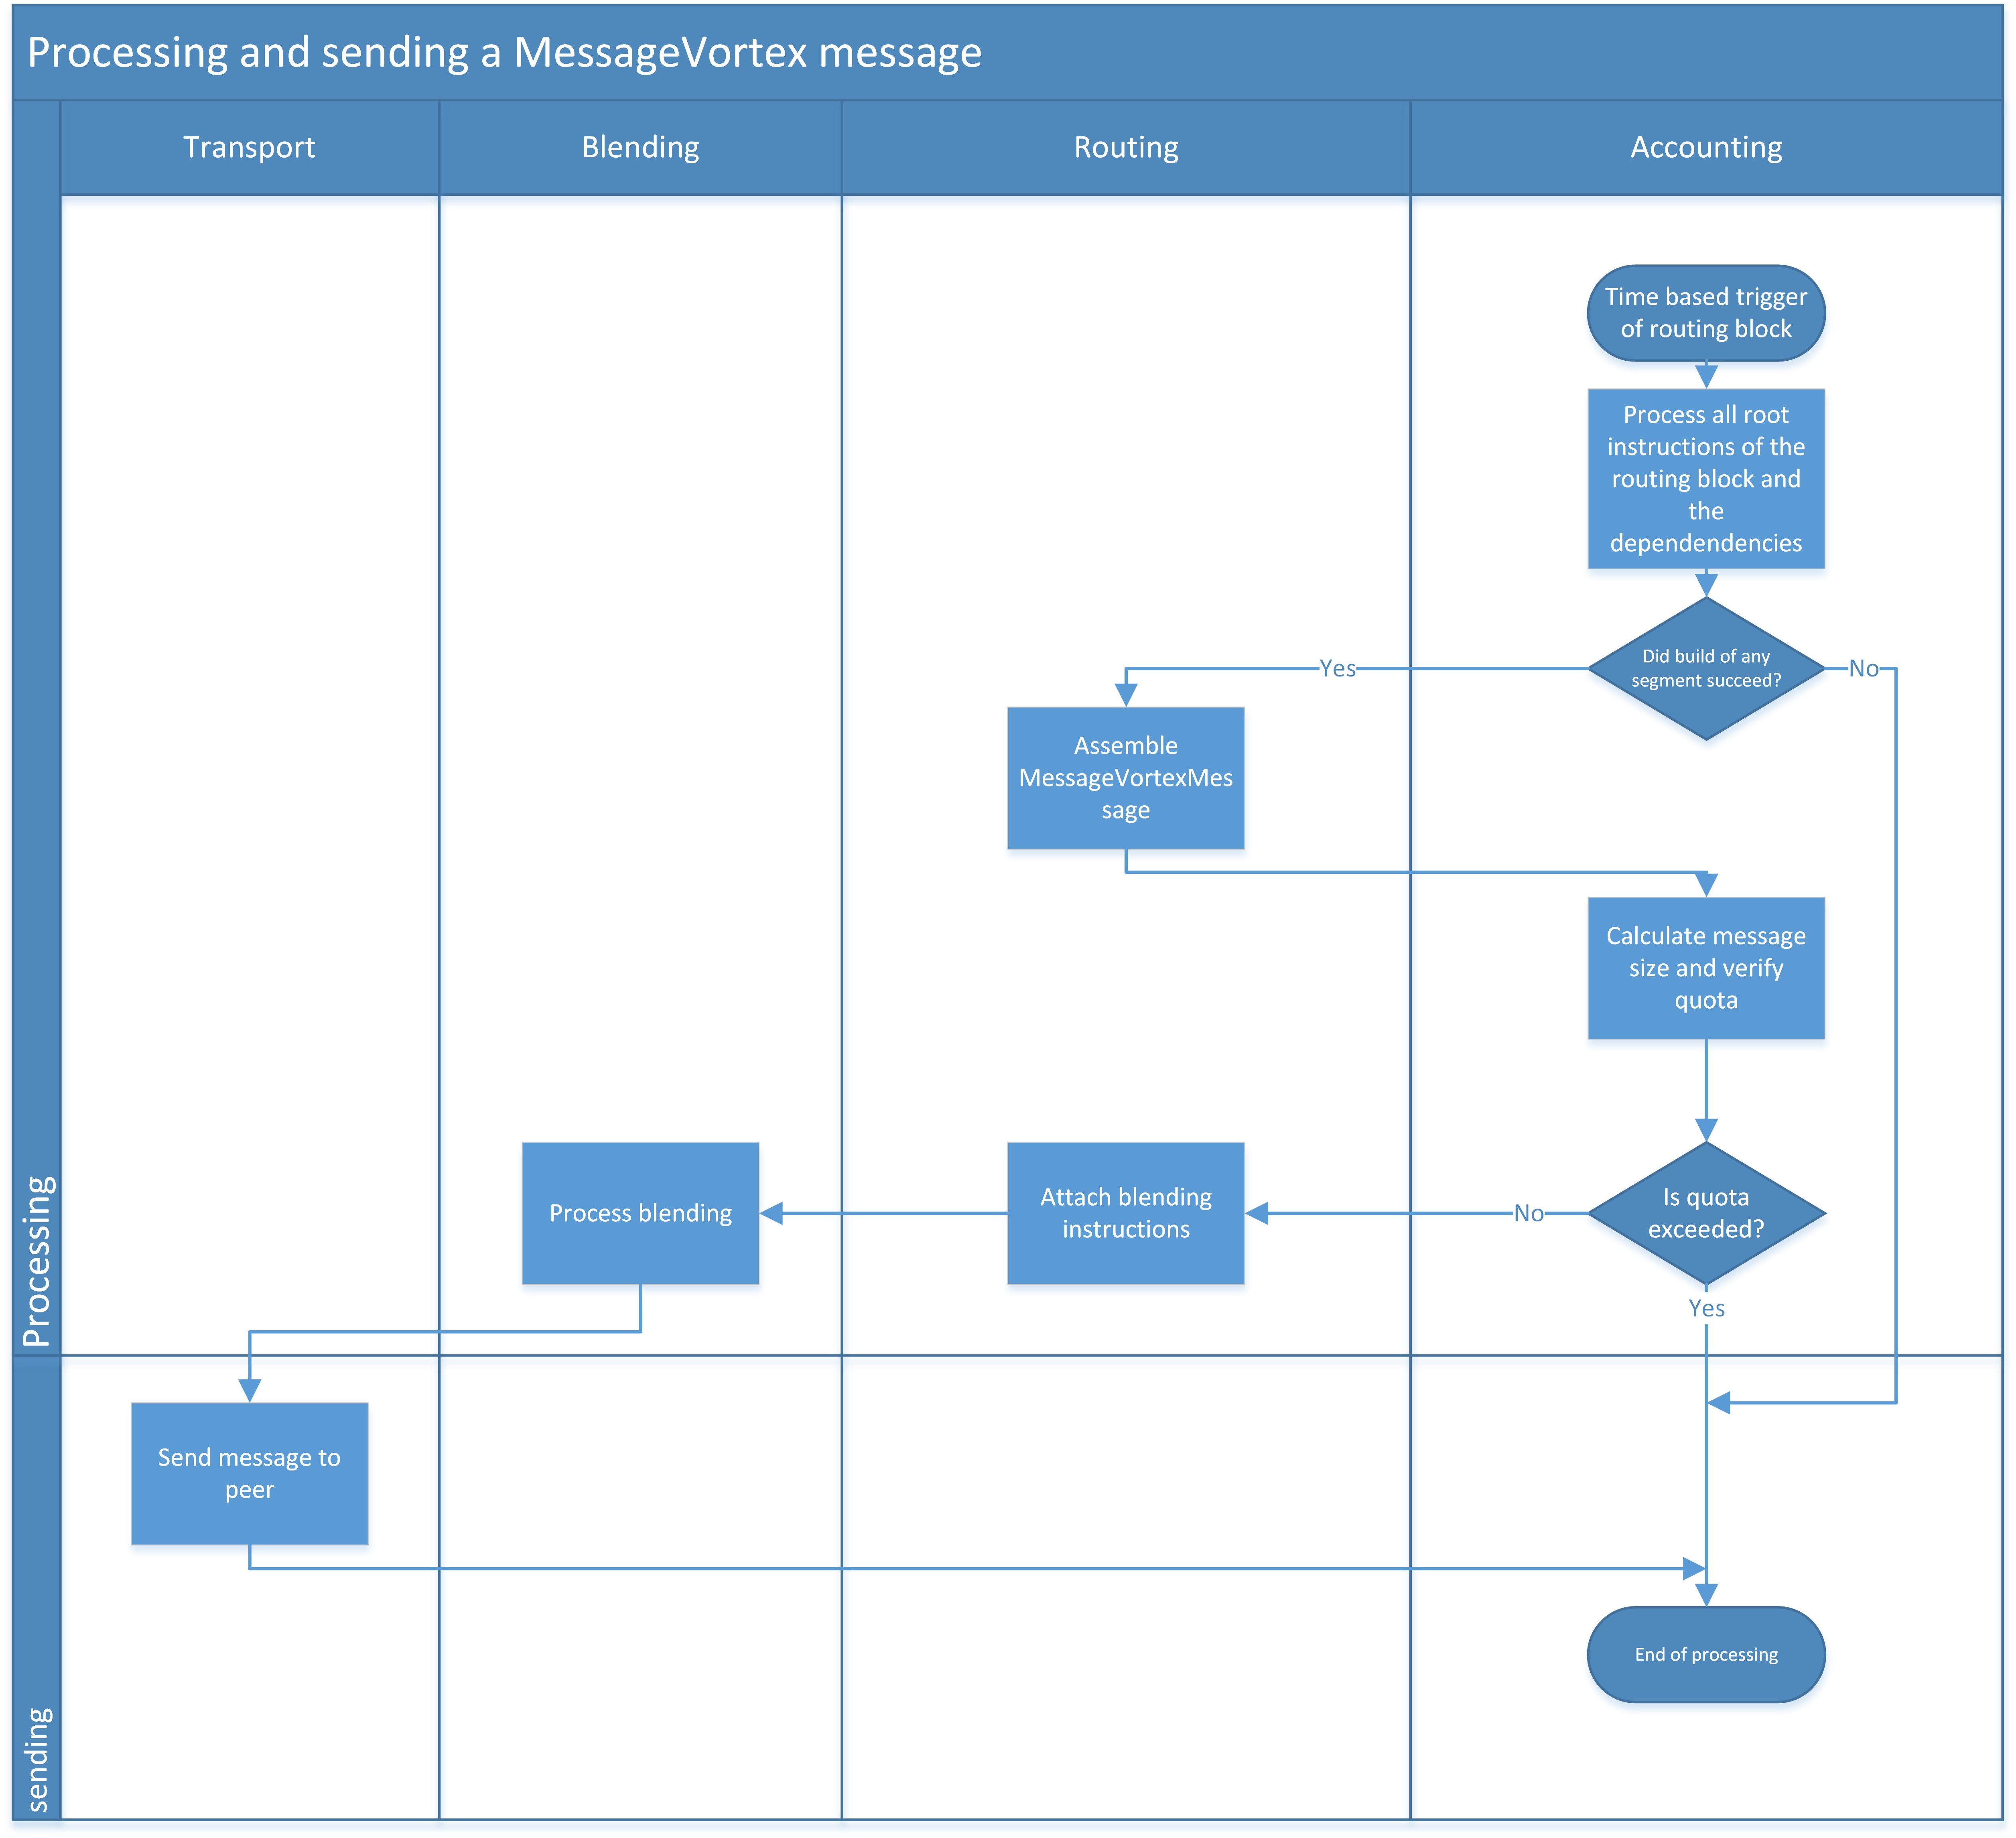
\includegraphics[width=0.90\textwidth]{inc/flowchart_message_sending}
	\caption{flow diagram showing processing of outgoing messages}
	\label{fig:msgSendProcessing}
\end{figure*}

\section{Sub Research Questions Roundup}
We sum up the findings of the last part regarding our three research questions and describe the next steps to be taken.

\subsection{SQ1: Technologies for sending messages maintaining unlinkability against an adversary}
We were unable to identify a single technology that withstands our adversary model entirely. The technologies were either too simple to withstand an adversary (e.g., remailers), have substantial flaws affecting their reliability (e.g., most mixes and DC networks), an active adversary could sabotage them or do not scale.

We were able to describe a rough protocol that performs far better in almost all aspects of anonymity than the solutions described in the previous sections. This comparison was always made for the adversary model given in section \ref{sec:adversary}. If we assume that the constraints of trust (only trust in sender and recipient infrastructure, whereas we always have multiple recipients) are valid, we can make the following statements regarding anonymity and unlinkability:
\begin{itemize}
	\item If an adversary identifies all involved nodes of a message and identifies all the corresponding messages and controls, all nodes except for senders and recipients nodes, he can determine message frequency, maximum message size, and message peers.
	\item If an adversary can identify all involved $i$ nodes of a sending party while controlling $j$ nodes, then he may determine a $k$-anonymity set whereas $k=i-j$ for the message set and a maximum message frequency. 
	\item If an adversary is running a node, he may identify other nodes participating in the network by analyzing peer messages.
\end{itemize}

We may safely assume that a carefully crafted message within a standard message flow is therefore unlinked from the two message peers. An adversary running a node may identify over time, possibly participating nodes, if not operating in a closed group, but he will be unable to query or use such a node without the corresponding keys. He may be able to observe such nodes, possibly view their activity, but he is unable to match messages generated.

In the next section, we will further elaborate on this protocol and analyze it. We will focus on the question of whether it is possible to create a protocol that withstands our threat model.

\subsection{SQ2: Attacking unlinkability and circumvention}
In the previous part, we identified a lot of attack schemes used to attack the anonymity of a protocol or infrastructure. While not all are technical, technicality plays a major part. We identified:
\begin{itemize}
	\item Anonymity attacks
	\begin{itemize}
		\item Hotspot attacks
		\item Side-channel attacks
		\item Sizing analysis
		\item Bugging attacks
		\item Tagging and tracing attacks
		\begin{itemize}
			\item Peer discovering attacks
			\item Traffic flow attacks
		\end{itemize}
	\end{itemize}
	\item Availability and reliability attacks
	\begin{itemize}
		\item Denial of service (DoS) attacks
		\item Censorship attacks
	\end{itemize}
	\item Non-technical Attacks
	\begin{itemize}
		\item Credibility attacks
		\item Censorship attacks
	\end{itemize}
\end{itemize}

We identified several possibilities to circumvent the attack classes listed above. Some of them, such as the bugging attack, may be countered by design (e.g., by allowing only simple messages). Others can only be countered partially in reality (e.g., DDoS attacks). We will further elaborate on the protocol and then analyze the impact of every single attack on the protocol.

\subsection{SQ3: Attack Mitigation by design}
This SQ is a part of the previous question to a certain extent. We identified that reliability and trust are key factors to a protocol. Therefore, allowing a single point of failure (SPOF) or extending trust over central infrastructures is deadly for an anonymizing protocol. Undetectability is another crucial point ignored by almost all protocols except for some aspects of ToR and some advanced forms of remailers.

When elaborating on the protocol in the next part, we will focus on introducing designs that will prohibit actions endangering anonymity. In the Result section, we will focus on all attacks, which should be mitigated by design. 

%!TeX program=pdflatex
%!TeX encoding=utf8
%!TeX spellcheck = en_US
%!TeX root = ../../messageVortex.tex

\part{Results}
To verify the hypothesis made in this paper, and to analyse properties of the protocol in a real world scenario a library was implemented in Java which was capable of handling all message packets and the routing stack as a whole. The following paragraphs describe the protocol developed in general as a generic approach. Appendix \ref{app:rfcMessageVortexMain} gives the full ASN.1 representation of the protocol. 

It is important to notice that ASN.1 has no mean to express encrypted structures. Due to this fact we defined all encrypted fields as \verb|OCTET STRING|. 

The protocol is defined int the ASN.1 to support onionized information in an unencrypted form. This is meant for debugging purposes only. At no point should this possibility be used in a production environment.

The protocol described in the next chapter is independent from routing. We built a blending layer for SMTP. Layers for other protocols such as XMPP may be built similarly. The protocol may be extended by adding blending layers and their addressing schemes.

The Protocol outlined here is the final product and has undergone many development cycles. A lot of really useful features and capabilities such as a mechanism analoguous to the SMTP received headers were dropped as they were very useful but threatened security or anonymity.

\chapter{Protocol Overview}
The MessageVortex protocol described here is an onionizing protocol for asynchronus data transfer. The protocol itself is embbeded into a carrier protocol as binary information to avoid easy detection and make it hard to block traffic without blocking other legitimate traffic.

The Protocol implementation is described in the RFC document in \ref{app:rfcMessageVortexMain}. It contains all necessary information to build the protocol. It is published on the website \url{https://messagevortex.net/} and on the official IETF channels. Beside the RFC document additional documents and a reference may be found.

The data transferred is passed thru a number of mixes. The builder of a routing block (normally the sender) decides upon the following attributes:
\begin{itemize}
	\item Hops for the message and all decoy traffic.
	\item Timing behaviour respectively speed of the message.
	\item Decoy traffic generation.
	\item Set of possible recipients.
\end{itemize}

These decisions are compiled into a routing block structure which is onionized. This routing block may then be used to transfer a message of almost any size. This message is then sent to the involved mixes.

A mix may be just an intermediate station or the final target of a message. Only the recipient of a message is able to tell whether a message was intended for him or not. Any mix does a certain number of operations on a message. Considering the message, the timing and the operations applied a mix may extract the following informations:

\begin{itemize}
	\item IP of the sending mix.
	\item Size of the message received.
	\item Size of all processed sub blocks.
	\item Arrival time of a message.
	\item Ephemeral identity a message belongs to (ephemeral pseudonym to the routing block builder).
	\item Validity time of the message on the node.
	\item Operations applied to the message.
	\item Size of all blocks sent.
	\item IPs of the receiving mixes.
\end{itemize}

A mix always applies the operations requested in the building instructions to the received data. If this is not done properly the message may fail to transfer to its final destination. 

The operations to be applied on a message are chosen in such a way that they may or may not generate decoy traffic. This guarantees that a valid message may not be identified on the operations applied to the message.

Redundancy may be built in a routing block as well as progress indication.

In the taxonomy of \cite{Shirazi2018} this protocol would be classified as follows:

\begin{itemize}
	\item Network topology: full
	\item Network connection direction: unidirectional
	\item Network connection syncronization: asynchronous
	\item Network symmetry roles: hybrid
	\item Network symmetry topology: flat
	\item Network symmetry decentrallization: fully decentralized
	\item Routing network view: partial
	\item Routing updating: Event based
	\item Communication routing type: source routed\footnote{Only partially correct, as the routing block builder decides on the route. This builder is not necesarily identical to the sender.}
	\item Communication scheduling: fair
	\item Communication node selection determinism: probabilistic
	\item Communication node selection set: user-based
	\item Communication node selection selection probability: uniform
	\item Performance latency: high
	\item Performance communication mode: message-based
	\item Performance implementation: yes
	\item Performances code availability: yes
	\item Performance context: email, messaging
\end{itemize}

\section{Vortex Message}
The outline in figure \ref{fig:messageOutline} is a simplified view onto the message block of MessageVortex.

\begin{figure*}[ht]
	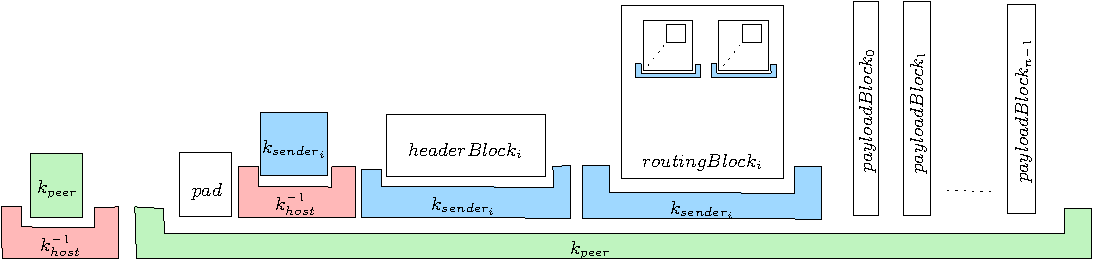
\includegraphics[width=\textwidth]{inc/blockLayoutSimplified}
	\caption{Simplified message outline}
    \label{fig:messageOutline}
\end{figure*}

A vortex message is a message passed from one mix to another this message may or may not contain any valuable information. The message itself is embedded as binary data into a transfer protocol. Every Mix may decide for himself what kind of protocols and embedding mechanisms are supported.

A vortex message is always built out of these blocks:
\begin{itemize}
	\item header
	\begin{itemize}
		\item Encrypted message key.\\
			  Contains symmetrical key for decryption of follow up header information and payload blocks. Encrypted with host identity public key.
		\item Identity and ``proof of work'' information\\
		      Contains Requests, Proof of work sections, and header key
	\end{itemize}
	\item Encrypted payload blocks (encrypted with header key)
	\begin{itemize}
		\item Routing blocks (encrypted with message key)
		\begin{itemize}
			\item Next hop timing instructions
			\item Next hop routing blocks (encrypted)
			\item Next hop header
			\item Message build instructions.
			\item Next hop header key and spec.
			\item Next hop blending instructions.
		\end{itemize}
		\item Payload chunk blocks
	\end{itemize}
\end{itemize}

It is important to note that there are two symmetrical keys involved in encrypting and decrypting message headers. This is not a flaw in the protocol but necessary. 

The first key which is in a Vortex message is the message key. This key is only accessible with the private key of the node receiving the message. It allows decryption of the routing blocks and the header information. The sender of a message block is therefore not able to tell if a message contains one or more routing blocks. It is important to note that no other node should have access to this information. 

The second key is the header key located in the encrypted header. This key was chosen by the creator of the routing block containing the information. This key protects the inner structure of the Message. it makes it impossible for any node except the sending or the receiving node to detect the inner structure of the message. Without this key any independent observer with knowledge about the blending capabilities of a receiving node may;
\begin{itemize}
	\item easier identify the block structure.\\ 
	This remains the case regardless whether ASN.1 or length prefixed structures are used. If the structure of a vortex Message can be easily identified the messages may be logged or dropped.
	\item Identify the routing block size.\\
	The value of this information is only very limited as it only reflects indierctly the complexity of thr remaining routing information.
	\item Identify the number of payload blocks and their respective sizes. \\
	This is valuable information when following a traffic.
\end{itemize}

\subsection{Key Usage}
Several keys are being used during the life of a message. In the following section we emphasize on type, usage and their specialities.

\subsubsection{Peer key}
The peer key is a message specific symetrical key known to two adjacent routing nodes. It is generated by the sending routing node and encrypted withthe public key of the receiving nodes identity key.

\subsubsection{Header Key}
The header key is a symmetric key protecting the routing and ephemeral identity information of the message. It is prepended to the header section and protected by the identity key of the processing node.

\subsubsection{Identity Key}
The Identity key is a static, asymetric keypair existing on a per user base used to sign messages or encrypt symmetric keys. We refer here as a user any peer participating in  message stream. Every user participating in the Vortex network requires at least one keypair. 

Depending on the usecase (eg. unlikable signatures or scalable security) a user may use multiple keypairs at the same time.

\subsubsection{Ephemeral Identity Key}
An ephemeral identity key identifies the sender to a processing host. The ephemeral identity key must be hadled in such a way that it is not linkable. It is manly used to process accounting information.

\subsection{VortexMessage Processing}
In order to process messages some FP arithmetic is required. To make sure that all implementations on all platforms behave exactly the same we always use arithmetic as specified in \cite{IEEE754}.

\subsubsection{Receiving Messages}
All messages are processed as follows:
\begin{enumerate}
	\item Extract length prefixed message key from block. Abort if not decryptable or invalid block.
	\item Decrypt message key with hosts private key $\rightarrow$ message key
	\item Extract length prefixed header message. Abort if too big.
	\item Decrypt header block with decrypted message key. Abort if not decryptable or invalid block.
	\begin{itemize}
		\item Verify identity
		\item Check quotas (if any)
		\item Extract header key
		\item Extract requests (if any)
		\item Check replays (if any)
	\end{itemize}
	\item Decide if message should be processed. If not abort here.
	\item Decrypt main block with message key
	\item Extract payload chunks.
	\item decrypt routing blocks with header key.
	\item Check backref secrets.
\end{enumerate}

Every routing block creates a new message.

The payload of a message is generated according instructions in the routing block. Timing instructions are relative to the arrival time of the message containing the routing block. This is necessary as a routing block may be used multiple times (see section \ref{sec:murb}).

A vortex message may be composed not earlier than a ``validFrom'' expressed in the respective routing block.

\subsubsection{Building and Sending Messages}
Any time after a routing block reaches ``vakidFrom'' and before the ``validTo'' is reached processing of a routing block is triggered. An implementation should when triggering a routing block for processing trigger as many routing blocks as possible to make traffic analysis harder.

The message is then built as follows:
\begin{enumerate}
	\item Check if all building instructions can be fulfilled due to their prerequisites.
	\item Build requested payload blocks.
	\item Extract peer key from routing block.
	\item Extract headerBlock from routing block.
	\item Extract (sender key encrypted) nextHop routing blocks from routing block.
	\item Encrypt message using the peer key.
	\item Update accounting figures.
	\item Blend into transport layer according to spec and send message.
\end{enumerate}

\section{Protocol design}
In this section we emphasize on the protocol blocks. These blocks are extracted from the blending layer and passed to the routing layer. A Vortex message is split into two main parts. The header block and the main block. The header block is divided into the two sub parts ``headerKey'' and ``identity block''. Although those blocks are described in \ref{app:rfcMessageVortexMainpp} as ASN.1 encoded structures they are not. In the message they are length prefixed fields.

In reality the structure of a message shown in \ref{fig:messageOutline} is as follows:
\begin{itemize}
	\item mPrefix size as 16 bit unsigned int (big endian)
	\item mPrefix bytes
	\item mainBlock size as 32 bit unsigned int (big endian)
	\item mainBlock bytes
\end{itemize}

The reason for not using ASN.1 encoding is that it might be possible to identify the unencrypted message on the transport layer as vortex message due to the ASN.1 structure. By switching to a length prefixed structure we make it impossible for an adversary to identify the unencrypted structures of a vortex message.

\subsection{Header block}
The header block contains the identity and should contain all information required to decide whether subsequent blocks of the message should be handled.

The header block contains the following data:
\begin{itemize}
	\item A symmetric header key (header key)\\
	This key is encrypted with the receiving identities public key. This key guarantees an efficient handling of the header data. As the number of bytes in the header is limited a receiving node may assign all subsequent work to a known identity or discard it.
	\item An identity block (identityBlock)\\
	This block contains a number of data which reflects the identity of the sender and the use of this (and subsequent blocks).
	\begin{itemize}
		\item sending ephemeral identity public key (identityKey)
		\item serial
		\item maximum number of replays for the serial for this identity
		\item Minimum number of seconds for replay protection.
		\item validity period for this block (in seconds)
		\item Symmetric decryption key for subsequent blocks
		\item Chain secret for the forwarding block\\
		If specified the specified secret should be named in all subsequent blocks.
		\item Protocol requests to this node
		\item Identifier and padding for proof of work
	\end{itemize}
	\item An identity signature (identitySignature)\\
	Contains a signed hash (hash type is specified in identityBlock.hash) with the senders private key.
\end{itemize}

\subsubsection{Ephemeral Identity}
The identity in this header block is an ephemeral identity. It exists for a limited amount of time (recommended <90d). Creating a new ephemeral identity is done with an identity request. This identity is mapped to all accounting figures.

\subsubsection{Requests\label{sec:request}}
Requests are always embedded in a header block. All requests are answered with a provided MURB (which is recommended to have a maximum replay value of 1).

There are several header requests defined:

\paragraph{newIdentity request:} This request may be answered with either a reject or a puzzle which is required to solve. Solving the puzzle results in the creation of the identity on the node. Identities may be rejected by the node for various reasons:

\begin{itemize}
	\item The node is not accepting newIdentity requests
	\item The identity is already taken.
	\item The identity is not strong enough (should be a longer key).
	\item The used encryption scheme is not supported by the node.
\end{itemize}

An identity may be rejected if the wrong types of keys and key sizes are used. However it must accept at least the key types and sizes it uses for its own identity.

If an identity is rejected the request may not be replayed by the same identity again. A sending party must generate a new identity for a new request. 

This request should be by far the most expensive request. It must at any time be more expensive to request a new identity compared to raise the quota of an existing one.

An identity is always ephemeral and expires after a given period of time. An identity may not be prolonged for security reasons. This oposes problems when using reply blocks. a reply block can only be valid as long as all included identities are valid. To counter this weakness without weakening security a ctxlessNewIdentity block may be sent to a reply block owner providing him with a new reply block.

\paragraph{queryPeer request:} A peer request is a request for publicly known Vortex nodes. This request does offer the possibillity of harvesting the Vortex network. To counter this the following limitations should apply:
\begin{itemize}
	\item The request should be very costly
	\item Only nodes avertising themselves as public are disclosed.
	\item Only one or two nodes should be disclosed upon request.
	\item The number of requests should be limited per identity.
	\item A node should always pick random nodes out of a 5\% pool of known Vortex addresses.
\end{itemize}

These measures limit the effectivity of harvesting attacks while giving a normal node the possibility of bootstrapping itself.

\paragraph{queryCapabillity request:} This request is the only request answered as a clear text request. To minimize probing possibilities this request should be only answered if the node owner agrees or generally by public nodes.

\paragraph{messageQuota request:} This request raises the number of routing blocks which may be processed for an identity. A node may reject this request depending on the load of the node, personal preferences, or because this identity causes too much traffic.

It is normally answered for all valid identities only. The node may answer it for recently expired identities. It is however not recommended to send a reply to an unknown identity as this behaviour might be used for probing of a node.

\paragraph{transferQuota request:} This request raises the number of bytes which may be transferred for an identity. A node may reject this request depending on the load of the node, personal preferences, or because this identity causes too much traffic.

It is normally answered for all valid identities only. The node may answer it for recently expired identities. It is however not recommended to send a reply to an unknown identity as this behaviour might be used for probing of a node.

\paragraph{queryQuota request:} This request instructs the node to send information about the given identity.

It is normally answered for all valid identities only. The node may answer it for recently expired identities. It is however not recommended to send a reply to an unknown identity as this behaviour might be used for probing of a node.

\subsubsection{Replys to Clear Text Requests}
It is up to the decision of the node whether it wants to answer a clear text request or not. Recommended for this behaviour is to discard plain text requests. 

This should only be a problem when bootstrapping or when adding new identities to the own address book. 

\subsection{Main block}
The main two block types are routing blocks and payload blocks. 

Routing blocks contain an onionised route chosen by the builder of the routing blocks and may contain instructions for building a message.

Payload blocks contain an encrypted message, parts of it or simply decoy traffic.

\subsubsection{Routing Blocks}
Routing blocks contain the following information:
\begin{itemize}
	\item The node specification of the next hop (requires a full identity; may be not there if no next hop)
	\item Purpose of routing block (May be normal/statusOK/statusError)
	\item The moment of processing as a range in seconds since the time of arrival.
	\item Retention time in seconds since the time of arrival.
	\item The identity block for the next hop
	\item The routing block for the next hop
	\item Payload ID to be included
	\item Payload building instructions (optional; only if MURB)
	\item A signing key for the payload (optional; only if MURB)
\end{itemize}

\subsubsection{Payload Building Instructions\label{sec:buildInstr}}
Payload is being built right before sending a block (processing a routing block). The building instructions are built as follows:
\begin{equation*}
srcIDs \xrightarrow{\text{build operation}} targetIDs
\end{equation*}

Every node maintains a list of received blocks including their IDs and building instructions for them. Any node must keep blocks and building instructions during the whole lifetime of a routing block. It may keep it longer. If a conflicting building instruction arrives all conflicting older rules are removed. Building instructions are always kept on a per-identity base. It is not possible to reference building instructions of a foreign identity.

\paragraph{splitPayload:} Split a message block into two parts of variable size. The size of the first chunk is expressed either absolute or in percent of the original block size.

\paragraph{mergePayload:} Concatenates two payload blocks of different or equal sizes.

\paragraph{encryptPayload:} Encrypts a payload chunk block with a given symmetric key and algorithm. Please note that this operation changes the size of a message due to the keysize and the padding.

\paragraph{decryptPayload:} Decrypts a payload chunk block with a given symmetric key and algorithm. Please note that this operation changes the size of a message due to the keysize and the padding.

All the operations specified above have in common that they may be applied on decoy traffic as well as on real message data. The size of incomming and outgoing blocks do not relate as there are messages increasing the size as well as decreasing the size.

\subsubsection{Reply Block\label{sec:replyBlock}}
Reply blocks are specialized blocks embedded into payload blocks. There are very few reply blocks necessary. Unlike normal data blocks these messages are not accounted in quotas on the node generating the reply block. 

It is up to the node to decide whether it wants to answer a request or not.

Replys are being built as an ordinary message blocks. To identify a Vortex message it must begin with the string ``\textbackslash special'' encoded in ASCII followed by a valid reply block structure. No additional bytes may be appended. Blocks with additional data should be discarded. To express a block starting with ``\textbackslash special'' the token is repeated prefixed with a backslash.

\paragraph{replyCapability block:}
The reply contains the following information:
\begin{itemize}
	\item Supported Vortex transports including blending specification.
	\item Maximum quota.
	\item Supported ciphers and hashes.
	\item Maximum number of simultaneous valid header serials.
	\item Maximum number of simultaneous valid building operations.
	\item Maximum identity lifespan in seconds.
\end{itemize}
It lists the capabilities a node advertises to the public. 

\paragraph{requirement block:}
Requirement blocks denote a requirement a requester has to fulfill before a previously sent request is processed. normally a proof of work puzzle has to be solved in order to allow a request to be processed. Alternatively a commercial supplier may request a payment in a digital currency. Currently supported digital currencies are Bitcon, Ethereum, and ZCash.

\paragraph{replyStatus block:}
General answer block signalling a a status. The block is limited in length in order to minimize misuse of bandwidth. The Block contains the following data:
\begin{itemize}
	\item Three digit status number
	\item Sending node identity
	\item Status text (optional)
	\item Affected block ID (optional)
\end{itemize}

\paragraph{ctxlessNewidentity block:}
This block may be used to signal the change of identity to a recipient. As this request is signed with the old known identity no means should exist to hijack such an identity.

This request contains:
\begin{itemize}
	\item old Identity
	\item new Identity
	\item Signature (with old identity)
\end{itemize}

This message may arrive at any time. Any recipient might decide on its own whether it wants to accept the update or not.

A node should not accept a identity update if the strength of the new identity has been lowered compared to the old identity. A client may make a difference on the fact whether the transport layer address or the key is exchanged. 

\subsubsection{payload Block}
The payload block contains the actual message or decoy traffic. Since this block is heavily modified in course of the transport of the block it is built very simple.

It contains:
\begin{itemize}
	\item A block ID
	\item The payload data
	\item A payload signature (optional; required for vortex blocks)
\end{itemize}

It is important to understand that a block may be exchanged at any time by an evil node. This however does not affect the safety on the message. Any tagging introduced at this point does invalidate the stream. The output after the next hop is completely unpredictable.

\subsection{Accounting\label{sec:accounting}}
Accounting covers several purposes in this system:
\begin{itemize}
	\item It makes the system costly for nodes sending bulk messages.
	\item It protects from replaying .
	\item It offers an ephemeral identity with a limited lifespan.
\end{itemize}

As accounting data may be used to overfill a nodes accounting tables special care has been taken in order to limit the number of information which has to be maintained per identity. We furthermore tried to minimize the risk that someone might occupy accounting memory of a node without costs. Furthermore any node may cancel an illict behaving identity at any time.

It is important that the accounting described here is for mixes. A node assembling messages needs to keep a lot more information.

\subsubsection{Accounting Data of an Identity}
For an ephemeral identity very little information has to be kept. This identity expires after a certain amount of time. The maximum time may be queried with a capability request. The choice of Encryption type and key size is left to the node requesting the identity. However, a node may reject the request if it considers the identity to be unsafe, it has no more capacity for new identities, or if it would create an identity clash on the current node.

The following data has to be kept per identity:
\begin{itemize}
	\item $\mathbf{ID}\langle pubKey, expiry, messagesLeft, bytesLeft \rangle$
	\item $\mathbf{Puzz[]}\langle expiry, request, puzzle \rangle$
	\item $\mathbf{Build[]}\langle expiry, targetID, buildOperation \rangle$
\end{itemize}
The $\mathbf{ID}$ tuple is the longest living tuple. It reflects an identity and exists as long as the current identity is valid. All other tuples are short living lists. As the server decides if he accepts new identities or not the size of this data is controllable.

$\mathbf{Puzz[]}$ is a list of not yet solved puzzles of this user. Every puzzle has a relatively short lifespan (typically below 1d). As the server may decide how many outstanding puzzles he accepts he controlls explicitely the size of this.

$\mathbf{Build[]}$ is a list of building instructions for a message. The server may decide at any time to reject a too big list or a too long living message. Thus he may control the size of this list as well. However, controlling the size of this list will most likely result in the non-delivery of a message.

\subsubsection{Accounting Data of a ``header'' Block}
All accounting data of a header block is connected to the respective identity. All header blocks do expire latest with their respective identity. The following data has to be kept on a mix:
\begin{itemize}
	\item $\mathbf{HL}\langle identity, serial, remainingReplays, expiry\rangle$\\
	This is the long term header list. It lists all headers of an identity, and how many replays are left until the requests are rejected.
	\item $\mathbf{HS}\langle identity, serial, arrivalTime, hash, duration \rangle$\\
	This is the short term replay protection. It protects a block with the same hash from being replayed.
\end{itemize}

\subsubsection{Accounting Data of a ``payload'' Block}
All accounting data is connected to a header block and expires latest with its header block. The expiry time is however relative to the arrival time of the header block.
\begin{itemize}
	\item $\mathbf{PL}\langle identity, serial, id, hash, expiry, content\rangle$\\
\end{itemize}

The $content$ may either be stored as th content or as the building instructions of the content as it is not always clear what block will be required for sending. A block may be defined for diagnostic paths only.

\subsection{VortexMessage Operations}
All operations are expressed as described in section \ref{sec:buildInstr}. The following sections give important details about the implementation of the operations.

\subsubsection{VortexMessage SplitPayload Operation}
The splitPayload operation splits a payload block into two chunks of different or equal sizes. The parameters for this operation are:

\begin{itemize}
	\item source payload block $pb_1$
	\item fraction $f$\\
	      Floatingpoint number describing the size of the first chunk. If fraction is 1 then the whole payload is transferred to the second target chunk
\end{itemize}

If $len(pb_1)$ expresses the size of a payloadblock called $pb_1$ in bytes then the two resulting blocks of the SpitPayload Operation $pb_2$ and $pb_3$ have to follow the following rules:

\begin{eqnarray}
split(f, pb_1) & = &\langle pb_1, pb_2 \rangle\\
pb_1.startsWith(pb_2)\\
pb_1.endsWith(pb_3)\\
len(pb_2) & = & floor(len(pb_1)\cdot f)\\
len(pb_1) & = & len(pb_2) + len(pb_3)
\end{eqnarray}

\subsubsection{VortexMessage MergePayload Operation}
The mergePayload operation combines two payload blocks into one. The parameters for this operation are:

\begin{itemize}
	\item first source payload block $pb_1$
	\item second source payload block $pb_2$
\end{itemize}

If $len(pb)$ expresses the size of a payloadblock called $pb$ in bytes then resulting block of the MergePayload Operation $pb_3$ have to follow the following rules:

\begin{eqnarray}
merge(pb_1, pb_2) & = & pb_3 \\
pb_3.startsWith(pb_1)\\
pb_3.endsWith(pb_2)\\
len(pb_3) & = & len(pb_1) + len(pb_2)
\end{eqnarray}

\subsubsection{VortexMessage XorSplitPayload Operation}
The xorSplitPayload operation forks payload block into two payload blocks. The parameters for this operation are:

\begin{itemize}
	\item Source payload block $pb_1$
	\item fraction $f$
	\item PRNG Initializer $pi$
\end{itemize}

If $len(pb)$ expresses the size of a payloadblock called $pb$ in bytes then resulting block of the MergePayload Operation $pb_3$ have to follow the following rules:

\begin{eqnarray}
xorSplit(pb_1, f, pi) & = & \langle pb_2,pb_3 \rangle \\
pb_2 & = & prng( i, floor(len(pb_1)\cdot f) )\\
pb_3 & = & pb_1 \oplus pb_2\\\
len(pb_2) & = & floor(len(pb_1)\cdot f)\\
len(pb_3) & = & max( len(pb_1), len(pb_2) )
\end{eqnarray}

For details about the implemented PRNGs see \ref{sec:prng}.

\subsubsection{VortexMessage XorMergePayload Operation}
The xorSplitPayload operation forks payload block into two payload blocks. The parameters for this operation are:

\begin{itemize}
	\item First source payload block $pb_1$
	\item Second source payload block $pb_2$
\end{itemize}

If $len(pb)$ expresses the size of a payloadblock called $pb$ in bytes then resulting block of the xorMergePayload Operation $pb_3$ have to follow the following rules:

\begin{eqnarray}
xorMerge(pb_1, pb_2) & = & pb_3 \\
pb_3 & = & pb_1 \oplus pb_2\\\
len(pb_3) & = & max( len(pb_1), len(pb_2) )
\end{eqnarray}


\subsubsection{VortexMessage EncryptPayload Operation}
The encryptPayload operation encrypts a payload block $pb_1$ symmetrically resulting in a block $pb_2$. The length of block $pb_2$ may vary according to mode and padding chosen. The parameters for this operation are:

\begin{itemize}
	\item Source payload block $pb_1$
	\item Encryption specification $spec$
	\item Symmetric key $k$
\end{itemize}

The operation follows the following rules (please note section \ref{sec:encNot} for notation):
\begin{eqnarray}
encrypt(pb_1, spec, k) & = & pb_2 \\
pb_2 & = & E_{spec}^{K_a}\left( pb_1 \right)\\\
len(pb_2) & \geq & len(pb_1)
\end{eqnarray}


\subsubsection{VortexMessage DecryptPayload Operation}
The decryptPayload operation decrypts a payload block $pb_1$ symmetrically resulting in a block $pb_2$. The length of block $pb_2$ may vary according to mode and padding chosen. The parameters for this operation are:

\begin{itemize}
	\item Source payload block $pb_1$
	\item Decryption specification $spec$
	\item Symmetric key $k$
\end{itemize}

The operation follows the following rules (please note section \ref{sec:encNot} for notation):
\begin{eqnarray}
decrypt(pb_1, spec, k) & = & pb_2 \\
pb_2 & = & D_{spec}^{K_a}\left( pb_1 \right)\\\
len(pb_2) & \leq & len(pb_1)
\end{eqnarray}

\subsubsection{VortexMessage addRedundancy and removeRedundancy Operation}
These operations build the core of the mixing operations. The operation allows to add to a padded message redundancy information or to rebuild a block from a chosen set of information. 

The Operation itself is shown in \ref{fig:addRedundancyOperation}. 
\begin{figure}[h]
	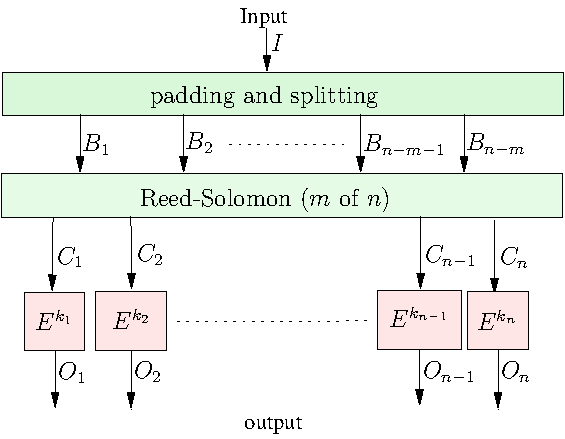
\includegraphics[width=\columnwidth]{inc/addRedundancyOp}
	\caption{Outline of the addRedundancy operation}
	\label{fig:addRedundancyOperation}
\end{figure}
It may be subdivided into the following operations:
\begin{itemize}
	\item Pad the original message block in such a way, that all resulting blocks are a multiple of the block size of the encrypting cypher.
	\item Apply a reed solomon operation in a given GF space with a vanderMonde matrix.
	\item Encrypt all resulting blocks with an unpadded symmetrical encryption.
\end{itemize}


\section{VortexMessage Request Processing}
Vortex message requests allow a Vortex node to gain knowledge about the Vortex network and, create new identities.

\fxwarning{add content here}

\subsection{VortexMessage Requests}
These requests are contained in the header portion of a Vortex message. These requests are purely for bootstrapping and maintaining the quota system and for requesting network capability.

The request information is defined in section \ref{sec:request}. For more information about the exact binary representation of all blocks and data see chapter \ref{sec:spec}.

Any node decides on its own what type of requests are being answered. 

A node not replying to clear text request is called a ``stealth node'' (see \ref{sec:stealthNode}). Such a stealth node discloses itself only to participants which do allready know at least the public key of the node. This usually means that they have ``earned'' this information by issuing a queryPeer request to another node and obtaining the information did already generate costs to the sender.

A node only replying to a fixed set of identities (in that specific case they are not ephemeral) is called a ``hidden node'' (see section \ref{sec:hiddenNode}).

It is recommended that unencrypted requests are not answered. A node may decide to answer unencrypted queryCapability requests in order to enable clients to bootstrap without (or with a minimal) network knowledge.

If a message contains $n$ requests in a header block it must supply at one reply blocks at the beginning of the routing block list. All reply blocks are concatenated and sent using the reply block. If the first block in the routing block list is not a reply block the request will fail.

\subsubsection{QueryCapability Request}
This request is primarily used to initialize a conversation with a node. It contains valuable information about the capability of the node as well as information about the embedding supported or the encryption. A node may or may not reply to a queryCapability requests. Doing so confirms the node to be participating in the vortex network.

The only valid reply is a replyCapability message in encrypted form.

\subsubsection{NewIdentity Request}
If this request is accepted it generates a new ephemeral identity. The identity itself is stored in the header fields. The standard behaviour is to reply with a replyPuzzleRequired block. 

This request generates a temporary ephemeral identity for the limited time denoted in the validity field of the reply block. No quota is assigned during that phase. As soon as the identity offers a valid puzzle solution the requested quota is assigned and the identity may be used for subsequent requests.

If a puzzle is not solved within the given time the temporary identity may be deleted. A node should not accept a solved puzzle after the given duration. 

Request with too high message or transfer quota requests should be answered with an replyPuzzleRequired block containing a zero length puzzle.

\subsubsection{QueryPeer Request}
As outlined in section \ref{sec:request} this request should be very costly and harvesting of known addresses should be hard. Furthermore this request should always  disclose the nodes from a fixed subset of the nodes known to the queried mix. This maximizes the effort to harvest participating nodes.

It is at the same time worth mentioning that this limit may oppose a thread that traffic is concentrated on similar nodes within participating nodes using the same initial set of known addresses to bootstrap. This due to the fact that if using the same node to bootstrap for multiple participants within a group results in peer knowledge which is similar. tThus resulting in a similar network. It is however also worth mentioning that participants belonging to more than one group will evolve over time as their different peer partners will result in different anonymity sets over time even when applying exact the same anr reproducaible rules.

\fxwarning{integrate sec query section from GIT here}

\subsubsection{TransferQuota, MessageQuota,  and QueryQuota Request}
This request may be accepted by a node if and only if the sender is a valid identity. It may be accepted even for a temporary identity.

The transfer quota offers the capability to raise the number of bytes an identity may transfer. This quota may be risen at any time. It is up to the owner of an ephemeral identity and the node using the identity to decide whether an identity may be kept or not respectively its quotas raised.

The Message Quota is a quota not limiting the number of bytes but the number of messages. As every message generates accounting overhead this number has to be limited as well. There are constraints similar to transferQuota when raising this value.

The queryQuota request enables the owner of an identity to query the current amount of remaining messages respectively bytes.

\subsection{VortexMessage Reply Blocks}
Reply blocks are as outlined in section \ref{sec:replyBlock} prefixed payload blocks. 

\subsubsection{ReplyCapability block}
The replyCapabilityBlock is the reply block to a queryCapability Request. The information provided here is outlined in section \ref{sec:replyBlock}. It is important to note that this block is even when requested in plain is always onionized and thus unreadable for third parties. 

A node may offer different capabilities to known identities than to anonymous clear text requests.

\subsubsection{replyPuzzleRequired block}


The replyPuzzleRequired block is the block reflecting the payment for a requested operation such as newIdentity, queryPeer, transferQuota, or messageQuota request.

Every puzzle block will create an accounting entry as outlined in section \ref{sec:accounting}. 

A node may reject an operation for any reason including exceeding an unnatural ammount of outstanding puzzles.

A reply containing a null length puzzle means that the requested operation is rejected.

\chapter{Vortex Prerequisites}
\section{Hardware}
No special Hardware is required for running Vortex nodes. The capabilities of Vortex are designed in such a way that ordinary mobile phones may act as vortex nodes. It is however recommended to have a node always connected to the internet. A mobile phone may disconnect from time to time based on the availability of the network. For our experiments we use a RaspberryPi Version 1. It is however recommended to use a faster, newer model due to the memory requirements of the proof of work algorithm.

The hardware currently requires a network interface and a fully functional JSE VM to run the reference implementation.

\section{Addresses}

\fxerror{change to one representation}

A Vortex address is built as follows: $vortexAddress=<transport>:<address>!<publicKey>$

To allow storage of Vortex addresses in standard messaging programs such as Outlook or Thunderbird. We define an alternate representation $encodedVortexAddress=base64(<transport>:<address>).<publicKey>@localhost$. 

The suffix ``@localhost'' makes sure that a message intended for Vortex is not routed by any non-participating server.

The main downside of vortex addresses are that they are no longer readable by a human. The main reason for this is the public key which is required. We may abstract this further by allowing clear text requests on the main email address for the public key. Such requests must then be answered by the vortex account with the valid Vortex address.

\subsection{Public Key Encoding in Address Representation}
The public key of an address is encoded as follows:
\begin{enumerate}
	\item The asymmetric key is encoded as specified in the AsymmetricKey in ASN.1
	\item The ASN.1 representation is then encoded using BASE64
\end{enumerate}	

\section{Transport Layers}                                          
As transport layer protocols we specified the protocols SMTP and XMMP as valid transport layers. In the following sections we specify the transport properties for these protocols.

\subsection{Embedding Spec}
Messages are always encoded as attachments in SMTP and XMMP. 

If not further specified by the receiving node an attachment should be the encoded message. 

Valid properties may be:
\begin{itemize}
	\item $ plainEncoding="("plain:"<numberOfBytesOfOffset>[,<numberOfBytesOfOffset>]*")$
	\item $ F5Encoding="(F5:"<passwordString>[,<PasswordString>]*")"$
\end{itemize}

All nodes responding to clear text should at least support $encoding=plain:0,256$.

\section{Client}
We did not create a Vortex client for sending messages. Instead we used a standard Thunderbird email client pointing to a local SMTP and IMAP Server provided by a Vortex proxy. On the SMTP side Vortex does encapsulate where possible mails into a Vortex message and builds automated route to the recipient. The SMTP part of vortex may be used to encapsulate automatically all messages with a known Vortex identity into a vortex message. On the IMAP side it merges a local Vortex message store with the standard Email repository building a combined view.

Using Vortex like this offers us the advantages of a known client with the anonymity Vortex offers.

This has certain downsides. At the moment the vortex client has only a local store this makes it impossible to handle multiple simulatneously connected clients to use Vortex. This is however just a lack of the current implementation and not of the protocol itself as we may safely use an IMAP storage for storing vortex mails centrally.

\subsection{Vortex Accounts}
By definition any transport layer address may represent a Vortex identity. This fact may make people believe that their current email or jabber address is suitable as Vortex address. This is technically perfectly true, but should not be done for the following reasons:

\begin{itemize}
	\item If an address is identified as a vortex address it may be blocked (directly or indirectly) by an adversary.
	\item If a vortex node is malfunctioning non-vortex messages should remain unaffected. This is more likely to happen if non-Vortex messages are kept in a separate account.
	\item If a user wants no longer to maintain its Vortex address (hopefully there will be a better technology in future) he just may give up his Vortex accounts. If he would have been using his normal messaging account for Vortex he would receive mixing messages which he has to filter in future.
\end{itemize}

\subsection{Vortex Node Types}

\subsubsection{Public Vortex Node}
Public nodes are nodes, which advertise themself as normal mixes. Just as all nodes they may be an endpoint or a mix. Typically they accept all requests exactly as outlined in \ref{tab:protoReplyCrit}. As an immediate result of the publicly available information about such a node the owner may be target of our adversary. Pressure may be oposed to close down such a node. However since we do not need a specific account we may safely close down one transport account and open up a different one. This is even possible on the same infrastructure. To notify other users of the move and remain reachable, a user may send an newIdentity request using the old identity. That way. we can guarantee, that only the holder of the old address may request an address update.

\subsubsection{Stealth Vortex Node\label{sec:stealthNode}}
This node does not answer any clear text requests. As an immediate result the node is only usable by other nodes knowing the public key of this node. The node is therefore on a known secret base only reachable.

\subsubsection{Hidden Vortex Node\label{sec:hiddenNode}}
A hidden node is a special form to a stealth node it has a set of preset identities. Only these entities are processed. This behaveour has certain drawbacks. An identity may not be changed. As an immediate result traffic may become a pseudonymity. To counter this effect at least partially we may use the same local identity for multiple senders. As an immediate result the sender is only one of all senders knowing the private key of an identity.

%===============================================================================================================

\chapter{MessageVortex - Transport Independent Messaging anonymous to \nth{3} Parties\label{sec:spec}}
This approach is different from all approaches discussed previously. Unlike them we put complete distrust into the infrastructure being used. Furthermore we do not rely on a custom server infrastructure in the internet. Instead we take advantage of the availability of internet connected devices such as internet connected mobile phones, tablets, or even commonly available SoC such as RaspberryPi or similar. It is still very hard to maintain a server in the internet and considering the vastly growing amount of automated attack carried out against internet connected servers it is not advisable or realistic to assume that a future user of this system owns either a server or connects to a service which is offering explicitly anonymizing services. These infrastructures would be suspectible to monitoring or even banning. Instead we take a different approach.

We use common messaging protocols as transport layers and connect to them using the respective client protocols. The actual mixes are operated by the users on their ``always connected'' devices. It goes without saying that such a system is far less reliable than a traditionally run server as this hardware is typically cheap and normally connected to the internet using a bandwidth shared media.

The basic idea is that a client generates all traffic (including decoy and diagnosis) by itself. It defines the routes a message takes through the mixes and decides which targets are receiving dummy traffic at the same time. In such a system, even when possessing all the nodes routing the traffic (without the endpoints) an anonymity set of $k$ (whereas the size of $k$ is defined by the sender) is guaranteed.

As decoy traffic is generated with the same operations as the true content is split it is impossible for an adversary running a node to determine whether he is generating noise or actually processing the true message.
All nodes, regardless of endpoint or mix implement the same logic and fulfil the same functions which makes it impossible to deteremine the function. Exit nodes as in Tor or similar systems do not exist.

\section{Accounting}
The Accounting layer maintains all local identities and controls overall load to the system. He processes requests from an ephemeral identity and generates replys to these requests. 

In table \ref{tab:protoReplyCrit} we show under what circumstances a reply to a header request should be sent. The capitalised words MAY, MUST, SHOULD and SHOULD NOT are used as defined in RFC2119\cite{RFC2119}.
\begin{table*}[h]
	\centering\scriptsize
	\begin{tabular}{|l|l|l|l|l|}\hline
		\diaghead{\theadfont Request Criteria}{Request}{Criteria} & \thead{unknown identity; cleartext} & \thead{unknown identity; encrypted} & \thead{expired identity; encrypted} & \thead{known identity; encrypted}\\\hline
		newIdentity	 	& SHOULD NOT 	& SHOULD NOT& Invalid (Error) 	& Invalid (Error)\\              
		queryPeer       & MUST NOT      & MUST NOT  & MAY               & MAY\\        
		queryCapability	& SHOULD NOT	& MUST 		& MUST				& MUST \\
		messageQuota	& MUST NOT 		& MUST NOT	& MAY				& MUST \\              
		transferQuota	& MUST NOT		& MUST NOT	& MAY				& MUST \\\hline             
	\end{tabular}	
	\caption{Requests and the applicable criteria for replies}
	\label{tab:protoReplyCrit}
\end{table*}
\fxwarning{Make sure that table matches RFC}

\section{Routing}
Routing of a message is simple. A workspace of an ephemeral identity contains routing blocks and payload blocks. A routing block has an active time window. Anytime during that time window a routing layer processes the routing instructions contained in the assembly operations of the routing block. If successful the message will be sent using the specified blending layer and target address.

\section{Blending layer}
Blending layer must be crafted in a careful manor. A blending layer is responsible for sensible content generation of the transport media plus embedding a VortexMessage into the transport layer according to specs provided by the original sender.

The original sender has no control over the plain text messages to avoid possibilities of sending targeted messages over the transport layer using MessageVortex. This differentiates MessageVortex from other systems having ``exit nodes'' such as Tor.

\subsection{Plain Inclusion}
The data stream has of the MessageVortex protocol has no structure visible from the outside. This property allows embedding as structureless information in files with a similar entropy. We did an analysis on common file formats in the internet to figure out which file format is suitable for this type of inclusion.

It is improtant to understand that this is very weak form of information hiding. A human observer may easily tell ``real'' data from ``broken'' data apart. A human is not able to tell whether a file is seriously broken or contains a VortexMessage.

\subsubsection{File Type Candidates}

We were unable to find any scientifical data regarding what type of traffic or attachment is common in the internet. We therefore tried to analyze mail logs (smtp) of a mail provider. We were scanning $567594$ emails for attachment properties after the spam elimination queue. $16.5\%$ of all scanned messages had an attachment. The top 20 attachment types distributions are shown in table \ref{tab:emailAttachments}.
\begin{table}[H]
%	\centering\scriptsize

\begin{tabular}{l|r}\hline
	Type																		& \%\\\hline
	image/jpeg                                                                  &	27.4\\
	application/ms-tnef	                                                        &	13.7\\
	image/png                                                                   &	13.3\\
	application/pdf                                                             &	10.7\\
	image/gif                                                                   &	7.4\\
	application/x-pkcs7-signature                                               &	5.4\\
	message/rfc822                                                              &	7.0\\
	application/msword                                                          &	3.1\\
	application/octet-stream                                                    &	3.0\\
	application/pkcs7-signature                                                 &	2.3\\
	application/vnd.\ldots.wordprocessingml.document	                        & 	1.4\\
	message/disposition-notification                                            &	1.1\\
	application/vnd.ms-excel                                                    &	0.8\\
	application/vnd.\ldots.spreadsheetml.sheet                                  &	0.6\\
	application/zip                                                             &	0.5\\
	application/x-zip-compressed                                                &	0.5\\
	image/pjpeg                                                                 &	0.4\\
	application/pkcs7-mime                                                      &	0.4\\
	video/mp4                                                                   &	0.4\\
	text/calendar                                                               &	0.4\\\hline
\end{tabular}
	\caption{Distribution of top 20 attachment types}
\label{tab:emailAttachments}
\end{table}
                    
As expected the amount of images within mail was very high ($\approx 50\%$). Unfortunately we were unable to analyze the content of ms-tnef attachments retrospectively. It seems that based on this figures information hiding within images in email traffic is a good choice.

\section{Considerations for Building Messages}
In a worst case scenario we assume that an adversary is controlling most of the network utilized for anonymisation. While this is not necessarily a problem, it allows an adversary to track a message while agents are being used under his control. So for simplicity and as a worst case assumption we always assume that an adversary has perfect knowledge of an associated message flow. This is however a worst case scenario. One missing agent disconnects the whole chain and as messages are no longer traceable.

\subsection{Ephemeral identities}
Any VortexMessage sender may maintain one or more ephemeral identites per node. These identities might be activee in parallel, overlapping, or even with interruptions. A routing block building node is advised to select a number of trustworthy nodes (such as known endpoints) and additionally some publicly available nodes or nodes obtained by bootstrapping. Those nodes are definitely not trustworthy and are ideally chosen from a list of different networks.

\subsection{Timing of messages}
Messages are flowing in a timed manor through the network. As a routing block builder has to take into account that potential routing mechanisms of the transport layer consume time, a message is delayed in each hop.  The timing and duration for delivery is controlled by the routing block builder. Depending on the number of hops for the longest path of the message and the delay windows on every hop the total message has a delay which is controllable by the routing block builder.

\subsection{Diagnostics}
To diagnose the flow of a message any part of the message may be sent directly or indirectly back to the routing block builder. This allows him to judge upon the message progress and whether nodes are well behaving or not.

There is no fingerprinting operation available for doing such diagnosis. Such operations would make the traffic identifiable as diagnostic traffic.

\subsubsection{Implicit Diagnostic}
When a message contains a routing block sending any parts back to the routing block builder, we call this implicit diagnostic. Any block built by the addRedundancy function may be seen as a kind of fingerprint over the whole message. A block sent back to the originating node may therefore reflect the message state up to this point and the way back.

\subsubsection{On-Demand Diagnostic}
Whenever a message fails or supectedly failed, a new routing block may be composed picking up parts of the message in workspaces anywhere within the participating nodes. This kind of diagnostic we call On-Demand diagnostic.

On demand diagnostic allows error conditions identified by implicit diagnostic to be tracked and narrowed down to the first offending node.

\section{Verification of requirements}
In the previous sections we identified a list of requirements.

In the following subsections we will iterate through all requirements and verify to what degree we achieved the goal.

\fxwarning{list all requirements; possibly missing one}

\paragraph*{\ref{req:zeroTrust}:} 
We have not put any trust into an external infrastructure. While we do assume that all routing nodes act as defined. A misbehaving node may be identified and eliminated without putting any trust on other nodes. Analysis have shown no means for a misbehaving node which might be intentional or unintentional endangering anonymity at any time. We do not rely on any third party technology or infrastructure for our anonymity. 

This requirement is therefore fulfilled.

\paragraph*{\ref{req:P2P}:} 
No node has additional privileges or offers additional services. All are equal and share the same privileges.

This requirement is therefore fulfilled.

\paragraph*{\ref{req:untagable}:} 
Messages may not be tagged. All content is either strictly onionised or defined and linked with unknown hooks. Tampering with a message will typically cause the message delivery to fail at the next node. Furthermore may tampering be detected.

This requirement is therefore fulfilled.
 
\paragraph*{\ref{req:unbugable}:} 
There are always means to bug a message. As we put trust in sender and recipient and we know already that a intermediate mixing node is not able to modify the message the protocol is hard to bug. There may be a possibility to bug a message with a routing log entry over DNS. If a recipient is not resolving names or trusts in the content of such a message he is safe.

This requirement is therefore fulfilled. May be only partially fulfilled if log entries are not handled with care.

\paragraph*{\ref{req:replay}:} Messages may only be replayed a limited amount of times. The number of replays is controlled by the sender and may not be altered by any mix. A malfunctioning mix replaying more often than allowed will not be able to extract any information than the information it obtained when sending the first time. 

This requirement is therefore fulfilled.

\paragraph*{\ref{req:accounting}:} 
All identities generated are not traceable as any identity is generated without any context and may not be mapped to an older or newer identity (perfect anonymous forward identity). Neither the source nor the replies may be used to be traced as all messages 

This requirement is therefore fulfilled.

\paragraph*{\ref{req:anon}:} Anonymity is hard to proof. 

The following statements are the findings of the previous chapters:
\begin{itemize}
	\item Routing nodes are identifiable by a deep inspection.\\
	      A routing node features unique features which can be identifyed. 
	      
	      Identifyable properties discovered are:
	      \begin{itemize}
	      	\item The usage of the plain embedding is identifyable by a human and using probabilistic approaches even by a scanner.
	      	\item A router is always connected and sends messages at any time of day
	      	\item A router is connected to multiple accounts
	      \end{itemize}
	\item A routing node is able to link a message to an ephemeral identity\\
	      This is a minor issue and is countered by the fact, that ephemeral identities have a very short lifespan and are unconnected.
	\item A routing node learns about other nodes over time.\\
	      A routing node is unable to communicate with the peers without a host key. It may however learn the endpoint address of its peer. Assuming a censoring adversary this may be a problem in a single case as the provider of the transport layer may be forced to block the account.
\end{itemize}

On the other hand, no node can tell by observing traffic if another node is a final recipient or just another router.

There are however some weaknesses in the protocol. As the implementation is currently connecting simultaneously to the transport layer endpoint (email or jabber account in the current implementation) and the Vortex account the user might be identified by that fact. Using a anonymisation proxy could solve the problem but it would violate the Zero trust principle.

A sender is capable to leak a receivers presence to a global observer.

This requirement is therefore only partially fulfilled. However, the weakness is very faint.

\paragraph*{\ref{req:boot}:} The header request peer functionality allows to query for routing nodes. The key handling of the protocol allows to use a node without disclosing its host key. Each node may decide on their own wether it leaks its own identity.

This requirement is therefore fulfilled.

\paragraph*{\ref{req:algVar}:} The protocol lists at least two completely independent algorithms of each kind to be supported. This allows switching if a algorithm has been broken. Wherever possible a well known algorithm and an algorithm basing on a completely different mathematical problem has been chosen.

This requirement is therefore fulfilled.

\paragraph*{\ref{req:easy}:} The protocol allows to reuse clients already available to send messages. The whole encryption and anonymity is hidden in a local proxy. This allows users to stick to their favorite tools.

This requirement is therefore fulfilled.

\section{Considerations for Routing Messages}
Messages should always be sent timewise nearby other messages. This means that the best moment for sending a message in a ready queue is at a time when sending of other messages is due. However no optimisation should be done to send as many messages as possible at the same time. this would lead to a forseeable behaviour of the routing layer and thus to misusable behaviour.

The approach is furthermore heavily dependent of the transport protocol and builds on top a new obfuscating/routing layer. For this system to become a real peer-to-peer approach some additional quirks are required. A message-Vortex-Account needs always an active routing handler. This routing handler may be introduced by new server capabilities or by having a device handling the routing from the client side. For this reason we built a RaspberryPi appliance capable of connecting to one (or more) accounts fetching incomming mails, analysing them and reroute them if necessary. Although the system is designed to be run on a RaspberryPi the software might be installed to any Java capable client. The RaspberryPi is just one affordable lightweight device which offers all required capabilities.

There was up until very late a routing log functionality in the protocol. This functionality did however have the disadvantage that it allowed bugging and could possibly  disclose intermediate mixes to a recipient which did not comply with the policy the mixes might have chosen. Therefore this feature was dropped and replaced with the fetch block behaviour.

The routing block builder controls the type of blending. Besides that he has no control over it. If blending is done carelessly a message can be easily detected and thus disrupted.

The message leakes the size when a routing block is reused. This is due to the version number and the ephemeral identity contained in the header. The message chunks reflect to a certain extend the message size in relation to the previous message sent.

\chapter{Security Analysis}
In the following sections we emphasize on attacks targeting either sender recipient tuples or on identification of participants. 

Based on the protocol we may safely assume the following key ponts:
\begin{itemize}
	\item An adversary knows and controls a significant number of nodes (for our analysis we assume less than 80\%).
	\item An adversary may observe the traffic at any point without getting any information about the message content
	\item An adversary is not capable of matching multiple messages on different nodes to one message.
\end{itemize}

We always assume an adversary to have more knowledge than we think he may extract from the messages.
\begin{itemize}
	\item We assume that an adversary knows all messages of a transaction running over his nodes and matches them correctly to the same message.
	\item 
\end{itemize}

We assume that the adversary is targeting the following informations:
\begin{itemize}
	\item Sender identity
	\item Recipient identity
	\item Message content
	\item Message size
\end{itemize}

Attacks on the users identity atre no longer possible as the identity used on the nodes is based on ephemeral identities instead of the users true identity. As the ephemeral identities may exist in parallel, overlapping or in a serial manor and are strictly unlinked to the true identity no statement can be made concerning the linking of ephemeral identities to the true identities. Frequency patterns or behavioral patterns may be split among multiple identities and distributed over multiple nodes. 

Frequency and bandwidth analysis are not possible as frequency and bandwith of a single message is not trackable and the size of a message is generally not related to the message flow. An exception to this statement is when routing a different message through a vortex system using a reused routing block general statements such as ``the message is bigger than the previous one'' about the messages size is possible if the routing block makes use of relative split operations. In experiments, we were able to mimic any desired communication pattern we wanted for an adversary to be found.

The message content remains cryptographically secured if the dual trust (sender and receiver node) is not broken, the message is encrypted on the senders node, the message is only decrypted on the receivers node, and remains at least wrapped in this encryption during the whole transfer. 

\subsection{Attacking Routing Blocks}
\fxwarning{add content here; Routing block length analysis}

\section{Attack on Message size}

\fxwarning{add content here}

\chapter{Additional Considerations}
\section{Man in the Middle Attacks to Conversations}

\fxwarning{add content here}

\section{Identification of Participating Nodes}

\fxwarning{add content here}

\subsection{Identification by Content}
It is possible to identify a message by content. Assuming that an adversary knows the applied blending method he may identify an ASN.1 structure of \fxerror{incomplete}

\fxwarning{add content here}

\subsection{Identification by Query}

\fxwarning{add content here}

\subsection{Identification by Traffic Type}

\fxwarning{add content here}

\subsection{Identification by Bandwidth}

\fxwarning{add content here}

\subsection{Identification by Behavioural Analysis}

\fxwarning{add content here}

\section{Storage of Messages and queues}
The storage of messages sent though MessageVortex should be handled with great care. It seems on the first sight a good idea to merge all messages in a globally available storage such as the IMAP account of the receiving entity. However -- In doing so we would discover the message content to the providing party of a mail account. Since we handled the message with great care and tremendous costs up until this point it would be careless doing so. 

Storing them in a localized and receiving entity controlled storage is definitely a good idea but leaves security considerations like a backup possibly to an end user. This might be better, but in effect a questionable decision. There is however a third option. By leaving the message unhandled on the last entity of the MessageVortex chain we may safely backup the data without disclosing the message content. Merging the content then dynamically through a specialized proxy would allow the user to have a unified view on his without compromising the security.

\fxwarning{implemented in prototype?}


%!TeX program=pdflatex
%!TeX encoding=utf8
%!TeX spellcheck = en_GB
%!TeX root = ../../messageVortex.tex

\part{Discussion \label{sec:discussion}}
In the following capters we analyze the protocol throughly for fitness of purpose. 

We first apply a statical analysis of the protocol to identify all informations leaked at all levels.

Then we apply a dynamic analysis of the protocol to identify all meta informations leaked during transmission of the protocol.

We then sum up the achieved goals by looking at well known attacks and analyze the effectiveness of them to analyze the protocol.

\chapter{Static analysis}
In this section we analyze statically the protocol. Looking at a full message we get the following Protocol outline:

\begin{eqnarray}
Inhalt...
\end{eqnarray}
\section{Transport and Blending Layer}

\subsection{Identifying a Vortex Message Endpoint}
Depending on the blending method, single messages might be identified as long as they are detectable. Detectability depends on various factors such as:

\begin{itemize}
	\item Broken internal file structure (due to plain blending)
	\item Uncommon high entropy in a structureless file
	\item Unrelated message flow (see \cite{oakland2013-parrot})
	\item Non-human behaviour on the transport layer (e.g., message traffic 24x7)
\end{itemize}

If an endpoint is successfully identified then all directly related endpoints of the same protocol may be identified as well by following the message flow. This does however not enable an adversary to inject messages as the hostkey is not leaked. 

Assuming a global observer as an adversary, he might discover the originating routing layer and thus identifying it as a Vortex node by following traces of the transport layer.

\section{Senders routing layer}
\fxfatal{A sender may have some knowledge about the Routing block size and may therefore guess the complexity of the routing path}

\section{Intermediate node routing layer}
\fxfatal{An intermediate node does know all the operations applied and the immediate next hop. It does learn an endpoint but is unable to use this endpoint.}
\fxfatal{An intermediate node may determine the relative message size.}

\section{Receivers routing layer}

\chapter{Dynamic analysis}
In the dynamic Analysis we reach out to an active adversary. An active adversary modifies traffic in a non protocol conformant way, or missuses available or obtained information to disrupt messages, nodes, or the system as a whole.

\section{Attacks against the vortex system itself}
An active adversary may attack the transport layer. Most of the transport layer are not able to reject message flooding. Therefore, it is easy to attack a transport layer with a flooding attack, such as a distributed denial of service (DDoS) attack. Due to the nature of the protocol we are unable to apply additional protection on the transport layer or below. The Vortex Message format itself is however crafted in such a way that only minimal effort is sufficient to get the involved parties. The Operations $ K_{msgN}=D^{K^{1}_{host}}\left(P\right)$ and $HEADER=D^{K_{msgN}}\left(H\right)$ are sufficient to identify message senders. Unknown Senders may be discarded without further processing. Known senders may be identified as legitimate and processed further. Known identities misbehaving may be discarded.


\subsection{DoS Attacks against the System}
An active adversary may not follow the protocol and modify any parts of the message. The following paragraphs reflect different kinds of behaviour and how they affect the messages and the system as a whole.

An adversary may not follow the blending specification. If he uses a specification which is less secure an independent third party observer may follow traffic. This is not sensible as such a node may send all the knowledge to such a collaborating node directly. In the case of a  target node not supporting the chosen blending method, the partial message path becomes interrupted. A possible redundancy in the path may recover the message from such a case.

\subsubsection{Traffic Replay}
Traffic replay is a common way to highlight traffic in many systems by replaying the same traffic and increase through this the signal to noise ratio of the system. 

Due to the replay protection of the vortex protocol it is not possible to of subsequent messages as the messages are terminated on the first conformal behaving node.

\subsection{Diagnosability of traffic}

\subsubsection{Hijacking of Header and Routing Blocks}
In order to Hijack a header or routing block, an attacker needs to know the forward secret which is contained within the encrypted data. Probability to generate such a

\subsubsection{Partial Implicit Routing Diagnosis}
\fxfatal{Write something about diagnosis and binary diagnosis without compromising anonymity}

\subsubsection{Partial Explicit Routing Diagnosis}
\fxfatal{Write something about diagnosis paths and their dangers if failing on their way forth and back}

\subsubsection{End-to-End Routing Diagnosis}
\fxfatal{Write something about receipt and their dangers if failing on their way back}

\subsubsection{Denial of Service by Exhausting Quotas or Limits}
\fxfatal{add more text here}

\section{Achieved Anonymity and Flaws}
\subsection{Measuring Anonymity}
\fxfatal{Write something about degree of anonymity and how to achieve or compromise}

\subsection{Attacking Anonymity through Traffic Analysis}
As traffic and decoy traffic and decoy traffic are chosen by the creator of the routing block frequency patterns can not be detected, unlike the router did create them. Same applies to message sizes and traffic hotspots. 
\fxwarning{Write more here}

\subsubsection{Attacking Anonymity through Timing Analysis}
\fxfatal{add more text here}

\subsubsection{Attacking Anonymity through Throughput Analysis}
\fxfatal{add more text here}

\subsection{Attacking Anonymity through Routing Block Analysis}
\fxfatal{add more text here}

\subsection{Attacking Anonymity through Header Analysis}
\fxfatal{add more text here}

\subsection{Attacking Anonymity through Payload Analysis}
\fxfatal{add more text here}

\subsection{Attacking Anonymity through Bugging}
\fxfatal{add more text here}

\subsection{Attacking Anonymity through Replay Analysis}
\fxfatal{add more text here}

\subsection{Attacking Anonymity through Tamper Replay Analysis}
\fxfatal{add more text here}

\chapter{Recommendations on using the Vortex Protocol}
\fxfatal{add more text here}

\chapter{Achieved Goals and Weaknesses}
Although the protocol was carefully designed it has certain flaws. These flaws typically assume that parts of the underlying security has been severely broken to be exploited.


\section{Message content}
Although it is possible to embed any type of content into a Vortex message great care should be taken as content may allow to disclose a readers identity or location. For this reason only self contained messages should be used (such as plain text messages).

\subsection{Splitting of message content}
\fxfatal{add more text here}

\subsection{Redundancy}
\fxfatal{add more text here}

\subsection{Redundancy Detection as Attack Pattern}
\fxfatal{add more text here}

\subsection{routing Considerations}
\fxfatal{add more text here}

\subsection{Hotspot Avoidance}
\fxfatal{add more text here}


\chapter{Anonymity}
\fxfatal{add content here}

\subsection{Size of the Anonymity Set}
\fxfatal{add more text here}

\subsection{Jurisdictional implications onto the Anonymity Set}
\fxfatal{add more text here}

\section{Effects of anonymous communication on behaveour}
\fxfatal{\cite{postmes2001social}}

\fxfatal{add content}



%\appendix
%\part{Appendix}

\onecolumn
\appendix
\pagenumbering{arabic}% resets `page` counter to 1
\renewcommand*{\thepage}{A\arabic{page}}
%\renewcommand{\setthechapter}{\Alph{section}}
%\renewcommand\thechapter{\Alph{chapter}}
%\setcounter{chapter}{0}



%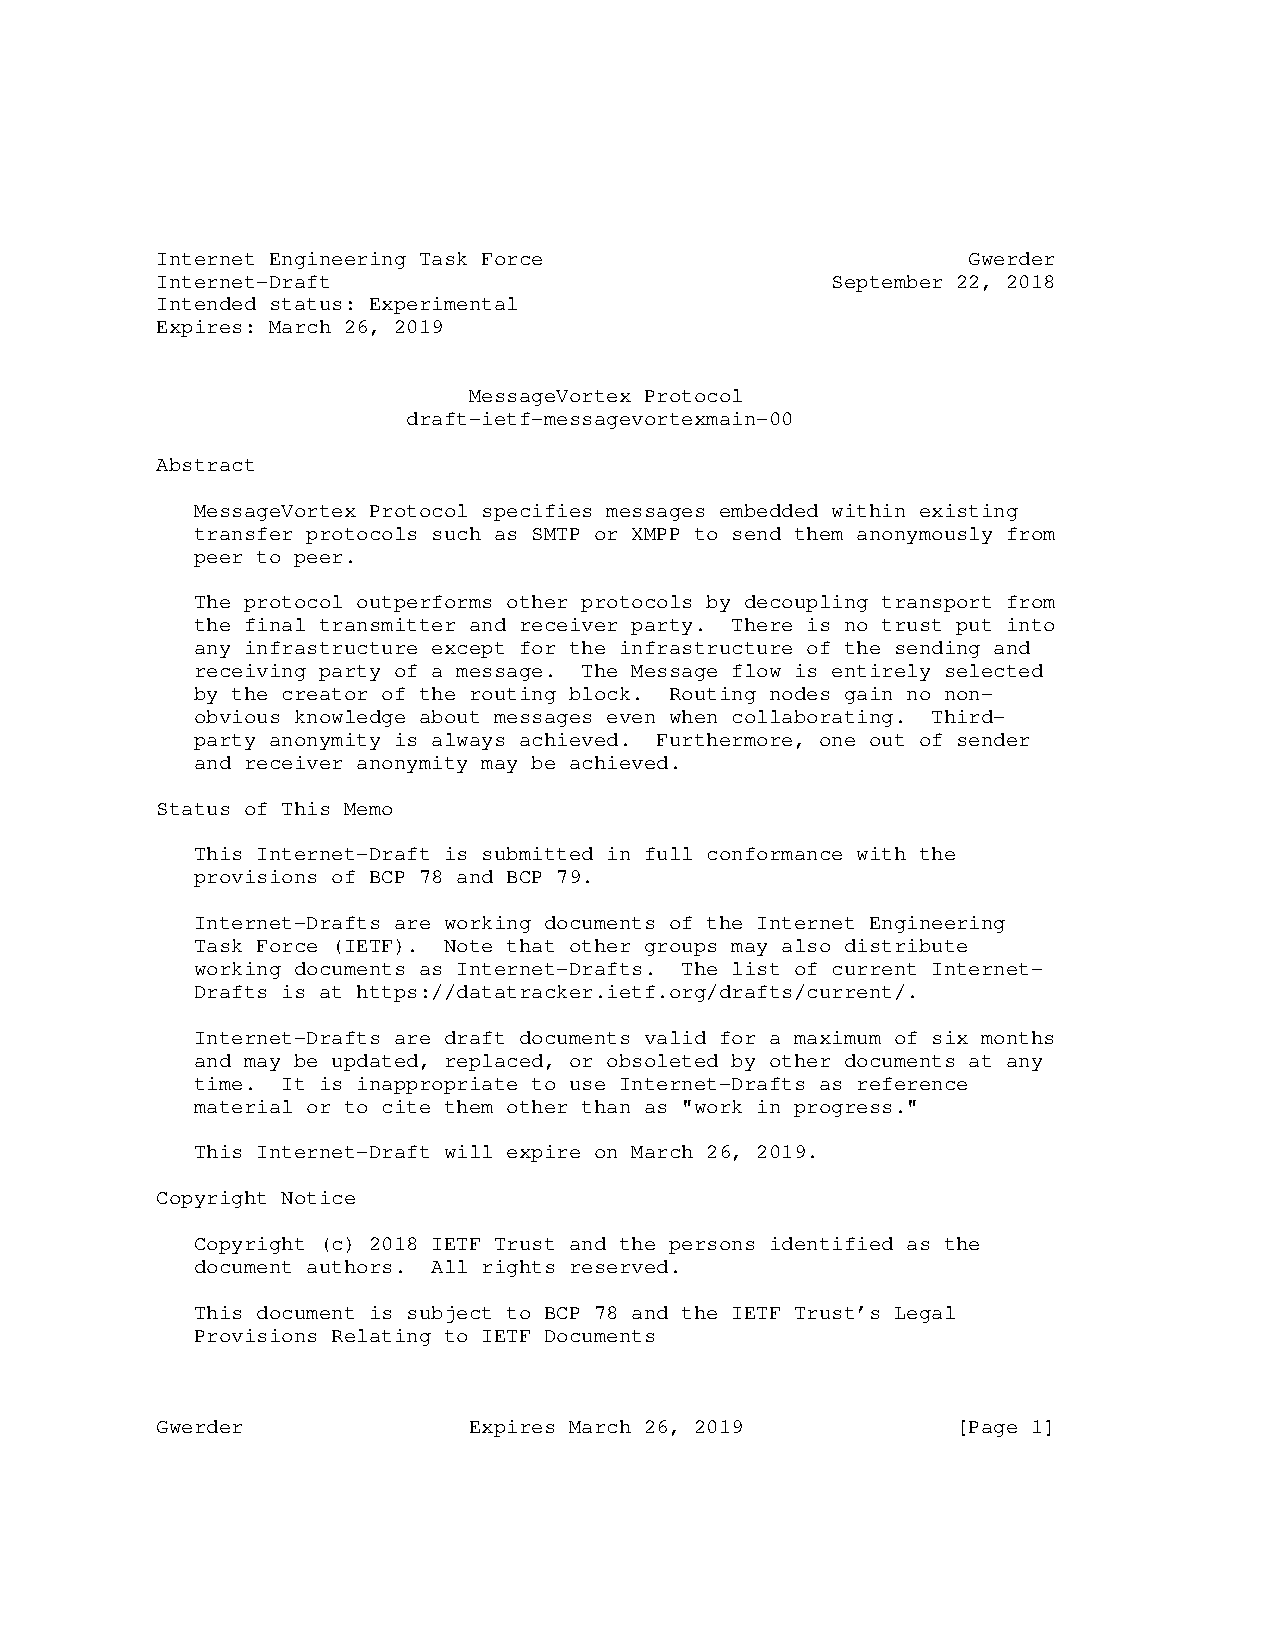
\includepdf[pages=-,frame=true,scale=0.5]{rfc/draft-gwerder-messagevortexmain-00.pdf}
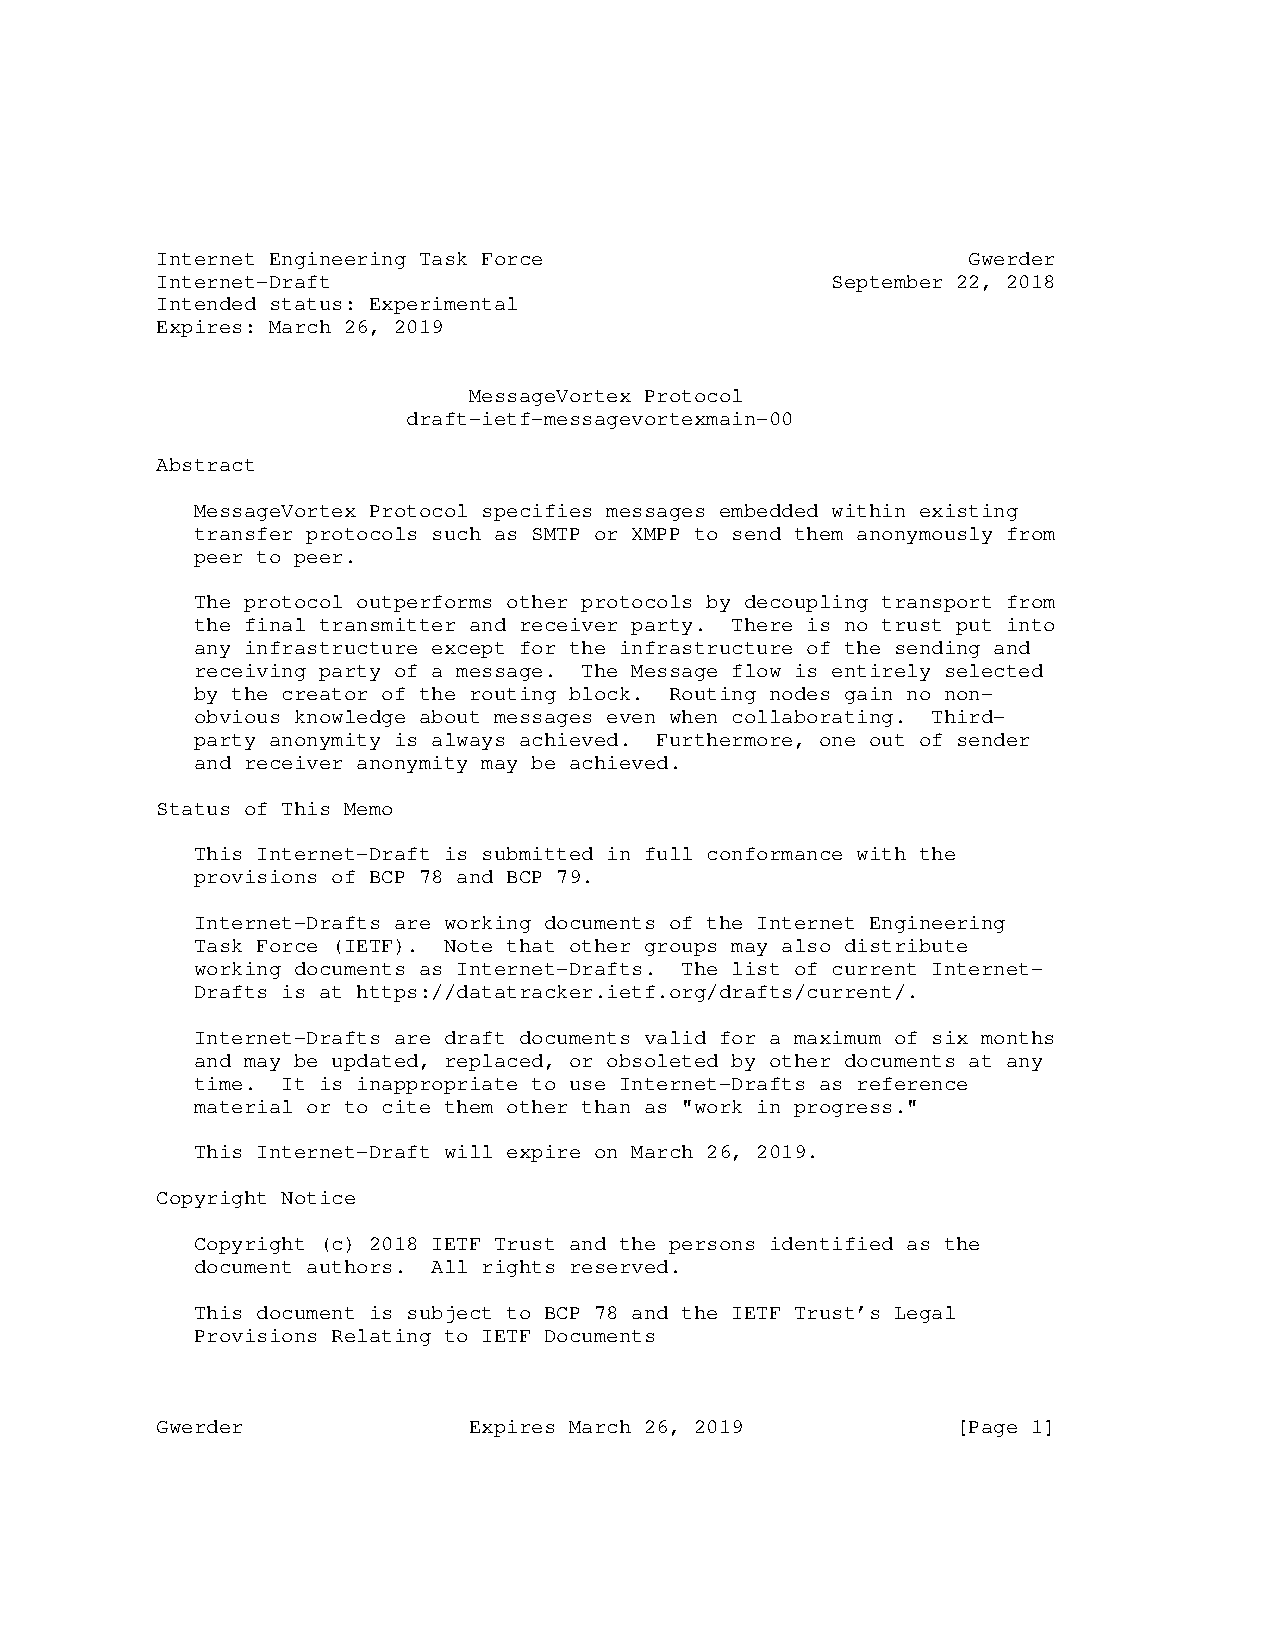
\includepdf[pages=1,frame=true,scale=0.75,pagecommand={\chapter{The RFC draft document\label{app:rfcMessageVortexMain}}}, offset=0 -1cm]{rfc/draft-gwerder-messagevortexmain-00.pdf}
\includepdf[pages=2-,frame=true,scale=0.8,pagecommand={}, offset=0 -1cm]{rfc/draft-gwerder-messagevortexmain-00.pdf}

\twocolumn
\chapter{Short analysis on common internet protocols}
The following sections list common internet protocols.

\section{HTTP}
The HTTP protocol allows message transfer from and to a server and is specified in RFC2616 \cite{RFC2616}. It is not suitable as a communication protocol for messages due to the lack of notifications. There are some extensions which would allow such communications (such as WebDAV) but in general even those are not suitable as they require a continous connection to the server in order to get notifications. Having a ``rollup'' of notifications when connecting is not there by default but could be implemented on top of it. 

HTTP servers listen on standard ports 80 or 443 for incomming connects. The port 443 is equivalent to the port 80 except for the fact that it has a wrapping encryption layer (usually TLS). The incomming connects (requests) must offer a header part and may contain a body part which would be suitable for transferring messages to the server. The reply onto this request is transferred over the same TCP connection containing the same two sections.

HTTP0.9-HTTP/1.1 are clear text protocols which are human readable (except for the data part which might contain binary data). The HTTP/2 (as specified in \cite{RFC7540}) is using the same ports and default behaviour. Unlike HTTP/0.9-HTTP/1.1 it is not a clear text but a binary protocol. Headers and bodies of messages are sent as binaries. 

To be a valid candidate as storage WebDAV support as specified in \cite{rfc4918} MUST BE ASSUMED

The protocol does definitely satisfy the first two main criteria (Ct1: Widely Adopted and Ct2: Reliable).

The main disadvantage in terms as message transport protocol is that this protocol is not symmetrically. This means that a server is always just ``serving requests'' and not sending actively information to peers. This Request-Reply violates criteria (Ct1: Symmetrically built) and makes the protocol not a primary choice for  message transport. 

\section{FTP}
FTP is defined in RFC959\cite{RFC959}. This Protocol is intended for authenticated file transfer only. There is a account available for general access (``anonymous''). This account does for security reasons normally not offer upload rights.

It is possible to use FTP as message transfer endpoint. The configuration would work as follows: ``anonymous'' has upload rights only. It is unable to download or list a directory. A node may upload a message with a random name. If there is a collision the node retries with another random name.

The blending layer picks messages up using an authenticated user.

This has multiple downsides. At first, handling FTP that way is very uncommon and usually requires an own dedicated infrastructure. Secondly passwords are within FTP always in plain text. This is considered as a very bad practice nowadays. Encryption as a wrapping layer (FTPS) is not common and SFTP (actually a subsystem of SSH) has nothing in common with FTP except for the fact that it may transfer files as well.

Furthermore FTP may be problematic when used in active mode for firewalls. All these problems make FTP not very suitable as transport layer protocol.

Like HTTP a main disadvantage of FTP in terms as a message transport protocol is that this protocol is not symmetrically. This means that a server is always just ``serving requests'' and not sending actively information to peers. This Request-Reply violates criteria (Ct3: Symmetrically built) and makes the protocol not a primary choice for  message transport. The Protocol however satisfies the first two criteria  (Ct1: Widely Adopted and Ct2: Reliable).

\section{TFTP}
TFTP has despite its naming similarities to FTP very little in common with it. TFTP is a UDP based file transfer protocol without any authentication scheme. This makes it not suitable as transport layer as it would leave messages open to anyone. The protocol is due to the use of UDP in a meshed network with reduntant routes. Since the internet has a lot of these redundant routes this neglects the use of this protocol.

TFTP is rarely ever used in the internet (it is quite commonly used in lans for booting over a network connection). This violates Criteria one (Ct1: Widely Adopted). TFTP is not symmetrically. This means that a server is always just ``serving requests'' and not sending actively information to peers. This Request-Reply violates criteria (Ct3: Symmetrically built) and makes the protocol not a primary choice for  message transport. The Protocol furthermore violates Ct2 (Ct2: Reliable) as it is based on UDP without any additional error correction.

\section{MQTT}
MQTT is an ISO standard (ISO/IEC PRF 20922:2016) and was formerly called MQ Telemetry Transport. The current standard as the time of writing this document was 3.1.1 \cite{mqtt}. 

The protocol runs by default on the two ports 1883 and 8883 and may be encrypted with TLS. MQTT is a publish/subscribe based message passing protocol which is mainly targeted to m2m communication. This Protocol requires the receiving party to be subscribed in a central infrastructure in order to be able to receive messages. This makes it very hard to be used in a system without centralistic infrastructure and having no static routes between senders and recipients.

The protocol does definitely satisfy the second criteria (Ct2: Reliable). It is in the area of enduser (i.e. Internet) not widely adopted thus violating Criteria 1 (Ct1: Widely Adopted). In terms of decentralistic design the protocol fails as well (Ct3: Symmetrically built).

\section{Advanced Message Queuing Protocol}
The Advanced Message Queuing Protocol (AMQP) was originally initiated by numerous exponents based mainly in finance related industries. The AMQP-Protocol is either used for communication between two message brokers, or between a message broker and a client\cite{amqp}.

It is designed to be interoperable, stable, reliable and safe. It supports either SASL or TLS secured communication. The usage of such a tunnel is controlled by the immediate sender of a message. In its current version 1.0 it does however not support a dynamic routing between brokers\cite{amqp}.

Due to the lack of a generic routing capability this protocol is therefore not suitable for message transport in a global generic environment.

The protocol satisfys partially the first criteria (Ct1: Widely Adopted), and fully satisfies the second criteria (Ct2: Reliable). However the third criteria is violated due to the lack of routing capabilities between message brokers (Ct3: Symmetrically built).

\section{Constrained Application Protocol (CoAP)}
The Constrained Application Protocol (CoAP) is a communication Protocol which is primarily destined to m2m communication. It is defined in RFC7252\cite{RFC7252}.  It is Defined as lightweight replacement for HTTP in IoT devices and is based on UDP.

The protocol does partially satisfy the first criteria (Ct1: Widely Adopted). The second criteria (Ct2: Reliable) is only partially fulfilled as it is based on UDP and does only add limited session control on its own.

The main disadvantage in terms as message transport protocol is that this protocol is not (like HTTP) symmetrically. This means that a server is always just ``serving requests'' and not sending actively information to peers. This Request-Reply violates criteria (Ct3: Symmetrically built) and makes the protocol not a primary choice for  message transport. 

\section{Web Application Messaging Protocol}
WAMP is a websockets based protocol destined to enable M2M communication. Like MQTT it is publish/subscribe oriented. Unlike MQTT it allows remote procedure calls (RPC).

The WAMP protocol is not widely adopted (Ct1: Widely Adopted) but it is definitely reliable on a per node base (Ct2: Reliable). Due to its RPC based capability unlike MQTT a routing like capability could be implemented. Symmetrical protocol behaviour is therefore not available but could be built in relatively easy.

\section{XMPP (jabber)}
XMPP (originally named Jabber) is a synchronous message protocol used in the internet. It is specified in the documents RFC6120\cite{RFC6120}, RFC6121\cite{RFC6120}, RFC3922\cite{RFC3922}, and RFC3923\cite{RFC3923}. The protocol is a very advanced chat protocol featuring numeros levels of security including end-to-end signing and object encryption\cite{RFC3923}. There is also a stream initiation extension for transferring files between endpoints \cite{xep0096}.

It has generic routing capabilities spanning between known and unknown servers. The protocol offers a message retrieval mechanism for offlin messages similarily to POP \cite{xep0013}.

The protocol itself seems to be a strong candidate as a transport layer as it is beeing used actively in the internet.

\section{SMTP}
The SMTP protocol is currently specified in \cite{RFC5321}. It specifies a method to deliver reliably asynchronous mail objects thru a specific transport medium (most of the time the internet). The document splits a mail object into a mail envelope and its content. The envelope contains the routing information which is the sender (one) and the recipient (one or more) in 7-Bit ASCII. The envelope may additionally contain optional protocol extension material. \par

The content should be in 7-Bit-ASCII (8-Bit ASCII may be requested but this feature is not widely adopted). It is split into two parts. These parts are the header (which does contain meta information about the message such as subject, reply address or a comprehensive list of all recipients), and the body which contains the message itself. All lines of the content must be terminated with a CRLF and must not be longer than 998 characters excluding CRLF.\par

The header consists of a collection of header fields. Each of them is built by a header name, a colon and the data. Exact outline of the header is specified in \cite{RFC5322} and is separated with a blank line from the body. 

It \cite{RFC5321} furthermore introduces a simplistic model for smtp message based communication. A more comprehensive model is introduced in the section \nameref{sec:mailTransport}. As the proposed model is not sufficient for a comprehensive end-to-end analysis.\par

Traditionally the message itself is mime encoded. The MIME messages are mainly specified in \cite{RFC2045}, and \cite{RFC2046}. MIME allows to send messages in multiple representations (alternates), and attach additional information (such as possibly inlined images or attached documents). 

SMTP is one of the most common messaging protocols in the internet (Ct1: Widely Adopted) and it would be devastating for business of a country if for censoring reasons this protocol would be cut off. The protocol is furthermore very reliable as it has built in support for redundancy and a throughout message design making it relatively easy to diagnose problems (Ct2: Reliable). All SMTP servers are normally capable of routing and and receiving messages. Messages going over serveral servers are common (Ct3: Symmetrically built) so the third criteria may be considered as fulfilled as well

SMTP is considered a strong candidate as transport layer.  

\section{SMS}
SMS capability was introduced in the SS7 protocol. This protocol allows the message transfer of messages not bigger than 144 character. Due to this restriction in size it is unlikely to be suitable for this type of communication as the keys beeing required are already sized similarly leaving no space for Messages or routing information.

Secondly the protocol is not widely adopted within the internet domain. There are gateways providing bridging functionalities to the SMS service. However -- the protocol itself is insignificant in the internet itself. 

\section{MMS}
The Multimedia Messaging Service (MMS) is maintained by 3GPP (\nth{3} Generation Partnership Project). This protocol is manly a mobile protocol based on telephone networks. This protocol is just like the SMS protocol accessible through the internet by using gateways but not directly usable within the internet.

\chapter{Glossary}

\begin{entry}
  \mainentry{adversary}{In this work we are referring to an adverser to any entity oposing to the privacy of a message. For a mor throughout definition refer to \ref{sec:adversary}}
\end{entry}

\begin{entry}
	\mainentry{anonymity}{We refer to the term anonymity as defined in \cite{anon_terminology}. ``Anonymity of a subject means that the subject is not identifiable within a set of subjects, the anonymity set.''\omitted}
	\subentry{Sender Anonymity}{The anonymity set is the set of all possible subjects. With respect to actors, the 	anonymity set consists of the subjects who might cause an action. With respect to actees, the anonymity set consists of the subjects who might be acted upon. Therefore, a sender may be anonymous (sender anonymity) only within a set of potential senders, his/her sender anonymity set, which itself may be a subset of all subjects worldwide who may send a message from time to time.}
	\subentry{Receiver Anonymity}{The same for the recipient means that a recipient may be anonymous (recipient anonymity) only within a set of potential recipients, his/her recipient anonymity set. Both anonymity sets may be disjoint, be the same, or they may overlap. The anonymity sets may vary over time.}
\end{entry}

\begin{entry}
  \mainentry{Agent}{An agent is a single component of a service (\defref{Service}) provided to a user or other services.}
\end{entry}

\begin{entry}
  \mainentry{EWS}{Exchange Web Services (EWS) are a Microsoft proprietary protocol to access exchange services from a client. It may be regarded as alternative to IMAPv4. This is however incomplete as EWS offers additional features such as User Configuration, Delegate Management or Unified Messaging.}
\end{entry}

\begin{entry}
  \mainentry{IMAP}{IMAP (currently IMAPv4) is a typical protocol to be used between a \defref{Client MRA} and a \defref{Remote MDA}. It has been specified in its current version in \cite{RFC3501}. The protocol is capable of fully maintaining a server based message store. This includes the capability of adding, modifying and deleting messages and folders of a mailstore. It does not include however sening mails to other destinations outside the server based store.}
\end{entry}

\begin{entry}
	\mainentry{Item of Interest (IoI)}{The Item of Intrest (IoI) are defined in \cite{anon_terminology} and refer to any subject action or entity which is of interest to a potential adversary.}
\end{entry}

\begin{entry}
  \mainentry{LMTP}{The Local Mail Transfer Protocol is defined in \cite{RFC2033}. This RFC defines a protocol similar to SMTP for local mail senders. This protocol allows a sender to have no mail queue at all and thus simplifies the client implementation.}
\end{entry}

\begin{entry}
  \mainentry{Local Mail Store}{A Local Mail Store offers a persistent store on a local non volatile memory in which messages are beeing stored. A store may be flat or structured (eg. supports folders). A Local Mail Store may be an authoritative store for mails or a ``Cache Only'' copy. It is typically not a queue.}
\end{entry}

\begin{entry}
  \mainentry{Server Admin}{We do regard a server admin as a person with high privileges and profound technical knowledge of a server and its associated technology. A Server Admin may have access to one or multiple servers of the same kind.}
\end{entry}

\begin{entry}
  \mainentry{MDA}{An MDA provides an uniform access to a local message store.}
  \subentry{Remote MDA}{A Remote MDA is typically supporting a specific access protocol to access the data stored within a local message store.}
  \subentry{Local MDA}{A Local MDA is typically giving local applications access to a server store. This may be done thru an API, a named socket or similar mechanisms.}
\end{entry}

\begin{entry}
  \mainentry{MRA}{A Mail receiving Agent. This agent receives mails from a agent. Depending on the used protocol two subtypes of MRAs are available.}
  \subentry{Client MRA}{A client MRA picks up mails in the server mail storage from a remote MDA. Client MRAs usually connect thru a standard protocol which was designed for client access. Examples for such protocols are POP or IMAP.}
  \subentry{Server MRA}{Unlike a Client MRA a server MRA listens passively for incomming connections and forwardes received Messages to a MTA for delivery and routing. A typical protocol supported by an Server MRA is SMTP}
\end{entry}

\begin{entry}
  \mainentry{MS-OXCMAPIHTTP}{Microsofts Messaging Application Programming Interface (MAPI) 
  	Extensions for HTTP specifies the Messaging Application Programming Interface (MAPI) Extensions for HTTP in \cite{ms-oxcmapihttp}, which enable a client to access personal messaging and directory data on a server by sending HTTP requests and receiving responses returned on the same HTTP connection. This protocol extends HTTP and HTTPS.}
\end{entry}

\begin{entry}
  \mainentry{MSA}{A Mail Sending Agent. This agent sends mails to a \defref{Server MRA}. }
\end{entry}

\begin{entry}
  \mainentry{MTA}{A Mail Transfer Agent. This transfer agent routes mails between other components. Typically  an MTA receives mails from an MRA and forwardes them to a MDA or MSA. The main task of a MTA is to provide reliable queues and solid track of all mails as long as they are not forwarded to another MTA or local storage.}
\end{entry}

\begin{entry}
  \mainentry{MTS}{A Mail Transfer Service. This is a set of agents which provide the functionallity tor send and receive Messages and forward them to a local or remote store.}
\end{entry}

\begin{entry}
  \mainentry{MSS}{A Mail Storage Service. This is a set of agents providing a reliable store for local mail accounts. It also provides Interfacing which enables clients to access the users mail.}
\end{entry}

\begin{entry}
  \mainentry{MUA}{A Mail User Agent. This user agent reads mails from a local storage and allows a user to read existing mails, create and modify mails.}
\end{entry}

\begin{entry}
  \mainentry{Privacy}{From the Oxford English Dictionary: ``
    \begin{enumerate}
      \item The state or condition of beeing withdrawn from the society of others, or from the public intrest; seclusion. The state or condition of beeing alone, undisturbed, or free from public attention, as a matter of choice or right; freedom from interference or intrusion.
      \item Private or retired place; private apartments; places of retreat.
      \item Absence or avoidance of publicity or display; a condition approaching to secrecy or concealment. Keeping of a secret.
      \item A private matter, a secret; private or personal matters or relations; The private parts.
      \item Intimacy, confidential relations.
      \item The state of being privy to some act.
    \end{enumerate}''\cite{OXFORD}\\
    In this work privacy is related to definition two. Mails should be able to be handled as a virtual private place where no one knows who is talking to whom and about what or how frequent (except for directly involved people).
  }
\end{entry}

\begin{entry}
	\mainentry{Pseudonymity}{
		As Pseudonymity we take the definition as specified in \cite{anon_terminology}.
		\begin{quote}
			A pseudonym is an identifier of a subject other than one of the subject's real names. The subject which the pseudonym refers to is the holder of the pseudonym. A subject is pseudonymous if a pseudonym is used as identifier instead of one of its real names.\omitted
		\end{quote}
	}
\end{entry}

\begin{entry}
  \mainentry{POP}{POP (currently in version 3) is a typical protocol to be used between a \defref{Client MRA} and a \defref{Remote MDA}. Unlike \defref{IMAP} it is not able to maintain a mail store. Its sole purpose is to fetch and delete mails in a server based store. Modifying Mails or even handling a complex folder structure is not doable with POP}
\end{entry}

\begin{entry}
  \mainentry{Service}{A service is a endpoint on a server providing a functionality to a client. This service may consist out of several Agents (\defref{Agent}).}
\end{entry}

\begin{entry}
  \mainentry{SMTP}{SMTP is the most commonly used protocol for sending mails across the internet. In its current version it has been specified in \cite{RFC5321}.}
\end{entry}

\begin{entry}
  \mainentry{Storage}{A store to keep data. It is assumed to be temporary or persistent in its nature.}
\end{entry}

\begin{entry}
	\mainentry{UBM}{We use the term Unsolicited Bulk Message as term for any mass message being received by a user without prior explicit consent. A less formal term for such a message in email terminology is spam or junk mail.}
\end{entry}

\begin{entry}
	\mainentry{Undetectability}{
		As undetectability we take the definition as specified in \cite{anon_terminology}.
		\begin{quote}
			Undetectability of an item of interest (IOI\index{Item of Interest}) from an attacker's perspective means that the
			attacker cannot sufficiently distinguish whether it exists or not.\omitted
		\end{quote}
	}
\end{entry}

\begin{entry}
  \mainentry{Unlikability}{We refer to the term uinlinkability as defined in \cite{anon_terminology}. ``Unlinkability of two or more items of interest (IOIs, e.g., subjects, messages, actions, ...) from an attacker’s perspective means that within the system (comprising these and possibly other items), the attacker cannot sufficiently distinguish whether these IOIs are 
  	related or not.}
\end{entry}

\begin{entry}
	\mainentry{Unobservability}{
		As unobservability we take the definition as specified in \cite{anon_terminology}.
		\begin{quote}
			Unobservability of an item of interest (IOI) means
			\begin{itemize}
				\item undetectability of the IOI against all subjects uninvolved in it and
				\item anonymity of the subject(s) involved in the IOI even against the other subject(s) involved in that IOI.
			\end{itemize}
		\end{quote}		
		As mentioned in this paper unobservability raises the bar of required attributes again ($\Rightarrow$ reads ``implies''):
		\begin{eqnarray*}
			censorship\ resistance & \Rightarrow & unobservability\\
			unobserability         & \Rightarrow & undetectability\\
			unobserability         & \Rightarrow & anonymity
		\end{eqnarray*}
	}
\end{entry}


\begin{entry}
	\mainentry{user}{Any human or technical entity using a system not following strict message processing rules. A user does always interface a non-interface related entity and is triggered by this or triggers it related, but not limmited, to the message.}
\end{entry}

\begin{entry}
	\mainentry{Zero Trust}{
		Zero trust is not a truly researched model in systems engineering. It is however widely adopted. We refer in this work to the zero trust model when denying the trust in any infrastructure not directly controlled by the sending or receiving entity. This distrust extends especially but not exclusively to the network transporting the message, the nodes storing and forwarding messages, the backup taken from any system except the client machines of the sending and receiving parties, and software, hardware, and operators of all systems not explicitly trusted. As explicitely trusted in our model we do regard the user sending a message (and his immediate hardware used for sending the message), and the users receiving the messages. Trust in between the receiving parties (if more than one) of a message is not necessarily given.
	}
\end{entry}		

\backmatter
\chapter{Bibliography}
{
  %\def\filespliter#1{\expandafter\intfilespliter#1\relax}
  %\def\intfilespliter#1 #2 #3\relax{ First: (#1), Second: (#2), Third: (#3) }
  \DeclareFieldFormat{file}{\StrGobbleLeft{#1}{1}[\wtcGwM]\StrGobbleRight{\wtcGwM}{4}[\filename] \IfFileExists{\filename}{\attachfile{\filename}}{FIXME missing document link}}
  \renewbibmacro{finentry}{\finentry\addspace \printfield{file}}
  \renewcommand*{\bibfont}{\small}
  \printbibliography[title={},heading=none]
}

% additional reference entries
\index{Mail transport|see {Message Transport}}

% add the index
\printindex

\begin{comment}
% just a trick to make TexNicCenter Bibliography working
\bibliography{messageVortex}
\bibliography{inc/bib/unclassified/Anonbib/anonbib}
\end{comment}




\chapter{Short Biography}
\begin{wrapfigure}{R}{0.3\columnwidth}
	\includegraphics[width=0.29\columnwidth]{inc/biography/passphoto}
\end{wrapfigure}
% !TeX spellcheck = en_GB

Martin Gwerder was born 20. July 1972 in Glarus, Switzerland. He is currently a doctoral Student at the University of Basel. After having concluded his studies at the polytechnic at Brugg in 1997, he did a postgraduate study as a master of business and engineering. Following that, he changed to the university track doing an MSc in Informatics at FernUniversit\"at in Hagen. While doing this he constantly broadened his horizon by working for industry, banking and government as  engineer and architect in security related positions. He currently holds a lecturer position for cloud and security at the University of Applied Sciences Northwestern Switzerland. His main expertise lays in the field of networking related problems dealing with data protection, distribution, confidentiality and anonymity.


\end{document}
